%
% Template Laporan Skripsi/Thesis Universitas Indonesia
%
% @author  Ichlasul Affan, Azhar Kurnia
% @version 2.2.1
%
% Dokumen ini dibuat berdasarkan standar IEEE dalam membuat class untuk
% LaTeX dan konfigurasi LaTeX yang digunakan Fahrurrozi Rahman ketika
% membuat laporan skripsi, yang kemudian diadaptasi oleh Andreas Febrian dan
% Lia Sadita untuk template skripsi tahun 2010.
% Konfigurasi template sebelumnya telah disesuaikan dengan
% aturan penulisan thesis yang dikeluarkan UI pada tahun 2017.
%


%
% Tipe dokumen adalah report dengan satu kolom.
%
\documentclass[12pt, a4paper, onecolumn, twoside, final]{report}
\raggedbottom

% Load konfigurasi LaTeX untuk tipe laporan thesis
\usepackage{_internals/uithesis}
%
\UseRawInputEncoding
% Load konfigurasi khusus untuk laporan yang sedang dibuat
%-----------------------------------------------------------------------------%
% Judul Dokumen
%-----------------------------------------------------------------------------%
%
% Judul laporan.
\def\judul{Pemantauan Kepatuhan secara Otomatis melalui Analisis Log pada Moodle Berbasis Kecerdasan Buatan}
%
% Tulis kembali judul laporan namun dengan bahasa Ingris
\def\judulInggris{Automated Compliance Monitoring through AI-Enhanced Log Analysis on Moodle}


%-----------------------------------------------------------------------------%
% Tipe Dokumen
%-----------------------------------------------------------------------------%
%
% Tipe laporan, dapat berisi: Laporan Kerja Praktik, Kampus Merdeka, Skripsi, Tugas Akhir, Thesis, atau Disertasi
\def\type{Skripsi}
%
% Nama jalur Kampus Merdeka (hanya perlu diisi jika tipe laporan adalah Kampus Merdeka
% Contoh isian (khusus Fasilkom): Studi Independen, Magang Mitra, Magang BUMN, Bangkit, Apple Academy, BYOC
\def\kampusMerdekaType{}
% Jika ada perwakilan mitra, isi dengan jabatan perwakilan mitra tersebut
% (misal: Cohort Manager)
% Kosongkan jika tidak ada perwakilan mitra
\def\partnerPosition{}
% Jika ada perwakilan mitra, isi dengan nama perusahaan atau nama program
% (misal: PT. Astra International, Bangkit Academy 2023)
% Kosongkan jika tidak ada perwakilan mitra
\def\partnerInstance{}
%
% Jenjang studi, dapat berisi: Diploma, Sarjana, Magister, atau Doktor
\def\jenjang{Sarjana}


%-----------------------------------------------------------------------------%
% Informasi Penulis
%-----------------------------------------------------------------------------%
%
% Tulis nama Anda
% Kosongkan penulisDua dan penulisTiga jika Anda melaksanakan tugas akhir/laporan secara individu
\def\penulisSatu{Yan Christofer Silalahi} % nama lengkap penulis pertama
\def\penulisDua{} % nama lengkap penulis kedua
\def\penulisTiga{} % nama lengkap penulis ketiga
%
% Tulis NPM Anda
% Kosongkan npmDua dan npmTiga jika Anda melaksanakan tugas akhir/laporan secara individu
\def\npmSatu{2106752464} % NPM penulis pertama
\def\npmDua{} % NPM penulis kedua
\def\npmTiga{} % NPM penulis ketiga
%
% Tulis Program Studi yang Anda ambil
% Kosongkan programDua dan programTiga jika Anda melaksanakan tugas akhir/laporan secara individu
\def\programSatu{Ilmu Komputer} % program studi penulis pertama
\def\programDua{} % program studi penulis kedua
\def\programTiga{} % program studi penulis ketiga
%
% Tulis Program Studi yang Anda ambil dalam bahasa inggris
% Kosongkan programDua dan programTiga jika Anda melaksanakan tugas akhir/laporan secara individu
\def\studyProgramSatu{Computer Science} % 1st author's study program
\def\studyProgramDua{} % 2nd author's study program
\def\studyProgramTiga{} % 3rd author's study program


%-----------------------------------------------------------------------------%
% Informasi Dosen Pembimbing & Penguji
%-----------------------------------------------------------------------------%
%
% Tuliskan pembimbing
% Untuk Kampus Merdeka: Tuliskan dosen PIC/pembimbing dari Fakultas Anda
\def\pembimbingSatu{Amril Syalim, S.Kom., M.Eng., Ph.D.}
% S1 s.d. S3: Kosongkan jika tidak ada pembimbing kedua
% Untuk Kampus Merdeka: Tuliskan penanggung jawab/penyelia/mitra
%                       dari program Kampus Merdeka yang Anda ambil (jika ada)
\def\pembimbingDua{}
% S2 & S3: Kosongkan jika tidak ada pembimbing ketiga
\def\pembimbingTiga{}

%
% Tuliskan penguji
\def\pengujiSatu{Penguji Pertama Anda}
\def\pengujiDua{Penguji Kedua Anda}
% Kosongkan jika tidak ada penguji ketiga (umumnya penguji ketiga hanya ada untuk S2)
\def\pengujiTiga{}
% Kosongkan jika tidak ada penguji keempat, kelima, atau keenam (umumnya penguji > 3 hanya ada untuk S3)
\def\pengujiEmpat{}
\def\pengujiLima{}
\def\pengujiEnam{}


%-----------------------------------------------------------------------------%
% Informasi Lain (Asal Fakultas, Tanggal, dsb.)
%-----------------------------------------------------------------------------%
%
% Tuliskan Fakultas dimana penulis berada
\def\fakultas{Fakultas Ilmu Komputer}
%
% Tuliskan bulan dan tahun publikasi laporan
\Var{\bulanTahun}{Juni 2025}
%
% Tuliskan gelar yang akan diperoleh dengan menyerahkan laporan ini
\def\gelar{Sarjana Ilmu Komputer}
%
% Tuliskan tanggal pengesahan laporan, waktu dimana laporan diserahkan ke
% penguji/sekretariat
\def\tanggalSiapSidang{09 Juni 2025}
%
% Tuliskan tanggal keputusan sidang dikeluarkan dan penulis dinyatakan
% lulus/tidak lulus
\def\tanggalLulus{Tanggal Bulan Tahun}


%-----------------------------------------------------------------------------%
% Judul Setiap Bab
%-----------------------------------------------------------------------------%
%
% Berikut ada judul-judul setiap bab.
% Silahkan diubah sesuai dengan kebutuhan.
%
\Var{\kataPengantar}{Kata Pengantar}
\Var{\babSatu}{Pendahuluan}
\Var{\babDua}{Studi Literatur}
\Var{\babTiga}{Metode Penelitian}
\Var{\babEmpat}{Eksperimen dan Analisis}
\Var{\babLima}{Kesimpulan}
\Var{\kesimpulan}{Penutup}


%-----------------------------------------------------------------------------%
% Capitalized Variables
% Anda tidak perlu mengubah apapun di bagian ini
%-----------------------------------------------------------------------------%
\Var{\Judul}{\judul}
\Var{\Type}{\type}
\Var{\PenulisSatu}{\penulisSatu}
\Var{\PenulisDua}{\penulisDua}
\Var{\PenulisTiga}{\penulisTiga}
\Var{\Fakultas}{\fakultas}
\Var{\ProgramSatu}{\programSatu}
\Var{\ProgramDua}{\programDua}
\Var{\ProgramTiga}{\programTiga}



% Daftar pemenggalan suku kata dan istilah dalam LaTeX
%
% Hyphenation untuk Indonesia
%
% @author  Andreas Febrian
% @version 2.1.2
% @edit by Ichlasul Affan, Muhammad Aulia Adil Murtito
%
% Tambahkan cara pemenggalan kata-kata yang salah dipenggal secara otomatis
% oleh LaTeX. Jika kata tersebut dapat dipenggal dengan benar, maka tidak
% perlu ditambahkan dalam berkas ini. Tanda pemenggalan kata menggunakan
% tanda '-'; contoh:
% menarik
%   --> pemenggalan: me-na-rik
%


% Silakan ganti ke bahasa Inggris (\selectlanguage{english}) jika Anda merasa terlalu banyak kata bahasa Inggris yang pemenggalannya tidak benar.
%\selectlanguage{english}


\hyphenation{
    % alphabhet A
    a-na-li-sa an-da a-tur a-tur-an
    a-pli-ka-si
    % alphabhet B
    bab ba-ngun-an
    be-be-ra-pa
    ber-fung-si
    ber-ge-rak
    ber-ke-lan-jut-an
    ber-o-per-ra-si
    ber-pe-nga-ruh
    bi-sa
    % alphabhet C
    ca-ri Com-po-nent-UML
    % alphabhet D
    di-da-pat-kan di-sim-pan di-pim-pin di-tam-bah-kan di-tem-pat-kan de-ngan da-e-rah di-ba-ngun di-gu-na-kan da-pat di-nya-ta-kan
    di-se-mat-kan di-sim-bol-kan di-pi-lih di-li-hat de-fi-ni-si di-de-fi-ni-si-kan di-mo-del-kan di-mi-li-ki di-re-a-li-sa-si-kan di-su-sun
    % alphabhet E
    eks-pli-sit e-ner-gi en-gi-neer en-gi-neer-ing eks-klu-sif ele-men
    % alphabhet F
    fa-si-li-tas
    fung-si fung-si-nya
    % alphabhet G
    ga-bung-an ge-rak ge-ne-ral ge-ne-ra-li-sa-si
    % alphabhet H
    ha-la-man
    ha-lang-an
    % alphabhet I
    in-fra-struk-tur i-ni-si-a-si
    % alphabhet J
    % alphabhet K
    ke-hi-lang-an
    ke-ter-hu-bung-an
    ku-ning
    kua-li-tas ka-me-ra ke-mung-kin-an ke-se-pa-ham-an
    ke-ti-dak-se-su-ai-an
    % alphabhet L
    ling-kung-an
    % alphabhet M
    ma-na-je-men me-neng-ah meng-a-da-kan me-mo-ni-tor
    me-mer-lu-kan me-mo-del-kan men-de-fi-ni-si-kan men-ja-di meng-ak-ses me-nam-bah-kan me-ne-mu-kan
    meng-a-tas-i me-mo-di-fi-ka-si me-mung-kin-kan me-nge-na-i me-ngi-rim-kan meng-i-zin-kan
    meng-u-bah meng-a-dap-ta-si me-nya-ta-kan me-nyim-pan me-res-trik-si mi-cro-ser-vi-ce mi-cro-ser-vi-ces mo-di-fi-ka-si mo-dul mo-dule
    meng-a-tur meng-a-rah-kan mi-lik meng-gu-na-kan me-ne-ri-ma me-nga-la-mi
    % alphabhet N
    nya-ta non-eks-klu-sif
    % alphabhet O
    o-pe-ra-si or-ga-ni-sa-si
    % alphabhet P
	pe-nye-rap-an
	pe-ngon-trol
    pe-mo-del-an
    pe-ran  pe-ran-an-nya
    pem-ba-ngun-an pre-si-den pe-me-rin-tah pe-mi-li-han prio-ri-tas peng-am-bil-an
    peng-ga-bung-an pe-nga-was-an pe-ngem-bang-an
    pe-nga-ruh pe-nge-lo-la pa-ra-lel-is-me per-hi-tung-an per-ma-sa-lah-an
    pen-ca-ri-an pen-ce-ta-kan peng-struk-tur-an pen-ting pen-ting-nya pe-ngu-ku-ran
    pre-sen-ta-si
    % alphabhet Q
    % alphabhet R
    ran-cang-an re-fe-ren-si re-pre-sen-ta-si
    % alphabhet S
    sub-bab si-mu-la-si sa-ngat ska-la-bi-li-tas
    stan-dar-di-sa-si
    % alphabhet T
    te-ngah
    ter-da-pat
    trans-for-ma-si
    % alphabhet U
    % alphabhet V
    va-li-da-si va-ri-an va-ri-a-si va-ri-a-bi-li-tas ve-ri-fi-ka-si
    % alphabhet W
    % alphabhet X
    % alphabhet Y
    % alphabhet Z
    % special
}

% Daftar istilah yang mungkin perlu ditandai
%
% @author  Andreas Febrian
% @version 2.2.1
% @edit by Ichlasul Affan
%
% Mendaftar seluruh istilah yang mungkin akan perlu dijadikan
% italic atau bold pada setiap kemunculannya dalam dokumen.
%
% v2.2.1 - support untuk Glossary (daftar istilah)
%

% Istilah/alias yang tidak perlu dimasukkan ke dalam Glossary/Daftar Istiilah
\var{\license}{\f{Creative Common License 1.0 Generic}}
\var{\bslash}{$\setminus$}


\makeglossaries

% Contoh istilah
\newglossaryentry{latex}
{
	name=\LaTeX,
	description={Sebuah \f{mark up language} yang didesain khusus untuk karya tulis ilmiah}
}

% Contoh Akronim
\newacronym{pdf}{PDF}{\f{Portable Document Format}}


% Awal bagian penulisan laporan
\begin{document}

%
% Sampul Laporan
%
%
% Sampul Laporan

%
% @author  unknown
% @version 2.2.0
% @edit by Andreas Febrian, Ichlasul Affan
%

\begin{titlepage}
	\begin{singlespace*}
	    \begin{center}
	        \begin{figure}
	            \begin{center}
	                
\includegraphics[width=2.5cm]{assets/pics/makara_kuning.png}
	            \end{center}
	        \end{figure}
	        \vspace*{-0.25cm}
	        \large
	        \bo{
	        	UNIVERSITAS INDONESIA\\
	        }
	
	        \vspace*{1.0cm}
	        % judul thesis harus dalam 14pt Times New Roman
	        \large
	        \bo{\Judul} \\[1.0cm]
	
	        \vspace*{2.5 cm}
	        % harus dalam 14pt Times New Roman
	        \large
	        \bo{\Type}
	
			% Sesuaikan spacing agar semua informasi muat dalam satu halaman 
	        \vspace*{3.5 cm}
	        
	        % penulis dan npm
	        \large
	        \ifx\blank\npmDua
		        \bo{\PenulisSatu} \\
		        \bo{\npmSatu} \\
	        \else
		        \bo{\PenulisSatu~/ \npmSatu~/ \ProgramSatu}\\
		        \bo{\PenulisDua~/ \npmDua~/ \ProgramDua}\\
	        \fi
	        \ifx\blank\npmTiga\else
	        	\bo{\PenulisTiga~/ \npmTiga~/ \ProgramTiga}\\
	        \fi
	        
	        % Sesuaikan spacing agar semua informasi muat dalam satu halaman 
	        \vspace*{6.25 cm}
	
	        % informasi mengenai fakultas dan program studi
	        \large
	        \bo{
	        	FAKULTAS \Fakultas\\
	        	PROGRAM STUDI \ProgramSatu \\
	        	DEPOK \\
	        	\bulanTahun
	        }
	        \normalsize
	    \end{center}
	\end{singlespace*}
\end{titlepage}

\ifodd\thechapterpagecount\forceclearchapter\fi


%
% Gunakan penomoran romawi untuk nomor halaman
%
\pagenumbering{roman}


%
% Halaman Judul Dalam
%
\strcompare{Kampus Merdeka}{\type}{} {
	\addtocontents{toc}{\protect\addvspace{-1em}}
	\addChapter{Halaman Judul}
	%
% Halaman Judul Laporan
%
% @author  unknown
% @version 2.2.0
% @edit by Andreas Febrian, Ichlasul Affan
%

\begin{titlepage}
	\begin{singlespace*}
	    \begin{center}
	    	\begin{figure}
	            \begin{center}
	                
\includegraphics[width=2.5cm]{assets/pics/makara_kuning.png}
	            \end{center}
	        \end{figure}
	        \vspace*{-0.25cm}
	        \large
	        \bo{
	        	UNIVERSITAS INDONESIA\\
	        }
	
	        \vspace*{1.0cm}
	        % judul thesis harus dalam 14pt Times New Roman
	        \large
	        \bo{\Judul} \\[1.0cm]
	
	        \vspace*{2.5 cm}
	        % harus dalam 14pt Times New Roman
	        \large
	        \bo{\Type} \\[0.5cm]
	        % keterangan prasyarat
	        \normalsize
	        Diajukan sebagai salah satu syarat untuk memperoleh gelar \\
	        \gelar\\
	
			% Sesuaikan spacing agar semua informasi muat dalam satu halaman 
	        \vspace*{4 cm}
	        
	        % penulis dan npm
	        \large
	        \ifx\blank\npmDua
		        \bo{\PenulisSatu} \\
		        \bo{\npmSatu} \\
		    \else
		    	\bo{\PenulisSatu~/ \npmSatu~/ \ProgramSatu}\\
		    	\bo{\PenulisDua~/ \npmDua~/ \ProgramDua}\\
		    \fi
		    \ifx\blank\npmTiga\else
			    \bo{\PenulisTiga~/ \npmTiga~/ \ProgramTiga}\\
		    \fi
		    
			% Sesuaikan spacing agar semua informasi muat dalam satu halaman 
	        \vspace*{4.25 cm}
	
	        % informasi mengenai fakultas dan program studi
	        \large
	        \bo{
	        	FAKULTAS \Fakultas\\
	        	PROGRAM STUDI \ProgramSatu \\
	        	DEPOK \\
	        	\bulanTahun
	        }
	        \normalsize
	    \end{center}
	\end{singlespace*}
\end{titlepage}

	\ifodd\thechapterpagecount\forceclearchapter\thispagestyle{onlypage}\fi
}


%
% Halaman Orisinalitas
%
\strcompare{Laporan Kerja Praktik}{\type}{} {
\strcompare{Kampus Merdeka}{\type}{} {
	\addtocontents{toc}{\protect\addvspace{-1em}}
    \addChapter{Halaman Orisinalitas}
	%
% Halaman Orisinalitas
%
% @author  Andreas Febrian
% @version 2.2.0
% @edit by Muhammad Aulia Adil Murtito, Ichlasul Affan
%

\chapter*{\uppercase{Halaman Pernyataan Orisinalitas}}
\vspace*{2cm}

% Untuk input gambar tanda tangan, silahkan sesuaikan xshift, yshift, dan width dengan gambar tanda tangan Anda
%\begin{tikzpicture}[remember picture,overlay,shift={(current page.north east)}]
%\node[anchor=north east,xshift=-8.5cm,yshift=-14.2cm]{
\includegraphics[width=3cm]{assets/pics/tanda_tangan_wikipedia.png}};
%\end{tikzpicture}
\pagestyle{onlypage}

\begin{center}
	\doublespacing
	\bo{\type~ini adalah hasil karya~\ifx\blank\npmDua{saya}\else{kami}\fi~sendiri, \\
	dan semua sumber baik yang dikutip maupun dirujuk \\
	telah~\ifx\blank\npmDua{saya}\else{kami}\fi~nyatakan dengan benar.} \\
	\vspace*{2.6cm}
	\setstretch{1.4}

	\begin{tabular}{l c l}
	\ifx\blank\npmDua
	\bo{Nama} & : & \bo{\penulisSatu} \\
	\bo{NPM} & : & \bo{\npmSatu} \\
	\bo{Tanda Tangan} & : & \\
	& & \\
	& & \\
	\else
	\bo{Nama Penulis 1} & : & \bo{\penulisSatu} \\
	\bo{NPM Penulis 1} & : & \bo{\npmSatu} \\
	\bo{Tanda Tangan Penulis 1} & : & \\
	& & \\
	& & \\
	\bo{Nama Penulis 2} & : & \bo{\penulisDua} \\
	\bo{NPM Penulis 2} & : & \bo{\npmDua} \\
	\bo{Tanda Tangan Penulis 2} & : & \\
	& & \\
	& & \\
	\fi
	\ifx\blank\npmTiga\else
	\bo{Nama Penulis 3} & : & \bo{\penulisTiga} \\
	\bo{NPM Penulis 3} & : & \bo{\npmTiga} \\
	\bo{Tanda Tangan Penulis 3} & : & \\
	& & \\
	& & \\
	\fi
	\bo{Tanggal} & : & \bo{\tanggalSiapSidang} \\
	\end{tabular}
\end{center}

\newpage

	\ifodd\thechapterpagecount\forceclearchapter\thispagestyle{onlypage}\fi
}}

% Memunculkan penomoran romawi untuk halaman-halaman awal
\pagenumbering{roman}


% Setelah bagian ini, halaman dihitung sebagai halaman ke 2 atau 3
\strcompare{Laporan Kerja Praktik}{\type}{\setcounter{page}{2}} {
	\strcompare{Kampus Merdeka}{\type}{\setcounter{page}{2}} {
		\setcounter{page}{3}
	}
}


%
% Lembar Pengesahan
%
\strcompare{Laporan Kerja Praktik}{\type}
{
	% Lembar Pengesahan Kerja Praktik dari LaTeX
	\addChapter{Lembar Persetujuan Dosen Kerja Praktik}
	%
% Halaman Pengesahan Laporan Kerja Praktik
%
% @author  Ichlasul Affan
% @version 2.1.2
% @edit by Ichlasul Affan
%

\chapter*{HALAMAN PERSETUJUAN DOSEN KERJA PRAKTIK}
\thispagestyle{empty}
\vspace*{0.4cm}
\noindent

\noindent
\begin{tabular}{ll p{9cm}}
	\multicolumn{3}{l}{\type~ini diajukan oleh:}  \\
	Nama&: & \penulisSatu \\
	NPM&: & \npmSatu \\
	Program Studi&: & \programSatu \\
	Judul Kerja Praktik&: & \judul \\
\end{tabular} \\

\vspace*{1.0cm}

\noindent \bo{Telah berhasil diselesaikan laporan kerja praktik untuk
Fakultas \fakultas~dan dipresentasikan hasil kerja praktiknya sebagai
persyaratan yang harus dipenuhi dalam mata kuliah Kerja Praktik.}\\[0.2cm]

\begin{center}
	DOSEN MATA KULIAH KERJA PRAKTIK\\[2cm]
\end{center}

\begin{center}
	\underline{\pembimbingSatu}\\[0.1cm]
\end{center}

\vspace*{2.0cm}

\begin{tabular}{ll l}
	Ditetapkan di&: & Depok\\
	Tanggal&: & \tanggalLulus \\
\end{tabular}

\newpage

	\ifodd\thechapterpagecount\forceclearchapter\thispagestyle{onlypage}\fi
}{
\strcompare{Kampus Merdeka}{\type}
{
	\addChapter{Lembar Pengesahan}
	%
% Halaman Pengesahan Laporan Kampus Merdeka
%
% @author  Ichlasul Affan
% @version 2.1.3
% @edit by Ichlasul Affan
%

\chapter*{LEMBAR PENGESAHAN}
\thispagestyle{empty}
\vspace*{0.4cm}
\noindent

\noindent
\begin{tabular}{ll p{9cm}}
	\multicolumn{3}{l}{Laporan Kegiatan Kampus Merdeka ini diajukan oleh:}  \\
	Nama&: & \penulisSatu \\
	NPM&: & \npmSatu \\
	Program Studi&: & \programSatu \\
	Judul Kegiatan&: & \judul \\
\end{tabular} \\

\vspace*{1.0cm}

\noindent \bo{Telah berhasil menyelesaikan program \kampusMerdekaType{} di bawah Kampus Merdeka, menyusun laporan akhir untuk Fakultas \fakultas, dan mempresentasikan hasil pekerjaannya sebagai persyaratan yang harus dipenuhi untuk melaksanakan transfer Satuan Kredit Semester (SKS) dari kegiatan tersebut.}\\[0.2cm]

\ifx\blank\pembimbingDua
	\begin{center}
		\bo{Dosen Pembimbing \kampusMerdekaType}\\
		\bo{\fakultas~Universitas Indonesia}\\[2cm]
	\end{center}
	
	\begin{center}
		\underline{\pembimbingSatu}\\[0.1cm]
	\end{center}
\else
	\begin{center}
		\begin{multicols}{2}
		\underline{\pembimbingSatu}\\[0.1cm]
		Dosen Pembimbing \kampusMerdekaType\\
		\fakultas~Universitas Indonesia\\
	
		\underline{\pembimbingDua}\\[0.1cm]
		\partnerPosition\\
		\partnerInstance\\
		\end{multicols}
	\end{center}
\fi

\vspace*{2.0cm}

\begin{tabular}{ll l}
	Ditetapkan di&: & Depok\\
	Tanggal&: & \tanggalLulus \\
\end{tabular}

\newpage

	\ifodd\thechapterpagecount\forceclearchapter\thispagestyle{onlypage}\fi
}
{
	\addChapter{Lembar Pengesahan}
	% Gunakan salah satu (comment atau hapus kode yang tidak perlu):
	% Lembar Pengesahan Tugas Akhir dari LaTeX
	\strcompare{Doktor}{\jenjang}
	{%
% Halaman Pengesahan Sidang (S3)
%
% @author  Andreas Febrian, Andre Tampubolon
% @version 2.1.2
% @edit by Ichlasul Affan
%

\chapter*{HALAMAN PENGESAHAN}
\thispagestyle{empty}
\vspace*{0.4cm}
\noindent

\noindent
\begin{tabular}{ll p{9cm}}
	\type~ini diajukan oleh&: & \\
	Nama&: & \penulisSatu \\
	NPM&: & \npmSatu \\
	Program Studi&: & \programSatu \\
	Judul \type&: & \judul \\
\end{tabular} \\

\vspace*{1.0cm}

\noindent \bo{Telah berhasil dipertahankan di hadapan Dewan Penguji
dan diterima sebagai bagian persyaratan yang diperlukan untuk
memperoleh gelar Doktor pada Program Studi \programSatu, Fakultas
\fakultas, Universitas Indonesia.}\\[0.2cm]

\begin{center}
	\bo{DEWAN PENGUJI}
\end{center}

\vspace*{0.3cm}

\begin{longtable}{l l p{7cm} l }
	\centering
	& & & \\
	Promotor&: & \pembimbingSatu & (\hspace*{3.0cm}) \\
	\ifx\blank\pembimbingDua
    \else
        & & & \\
    	Kopromotor&: & \pembimbingDua & (\hspace*{3.0cm}) \\
    \fi
    \ifx\blank\pembimbingTiga
    \else
        & & & \\
    	&: & \pembimbingTiga & (\hspace*{3.0cm}) \\
    \fi
	& & & \\
	Tim Penguji&: & \pengujiSatu~(Ketua) & (\hspace*{3.0cm}) \\
	& & & \\
	&: & \pengujiDua~(Anggota) & (\hspace*{3.0cm}) \\
	\ifx\blank\pengujiTiga
    \else
        & & & \\
    	&: & \pengujiTiga~(Anggota) & (\hspace*{3.0cm}) \\
    \fi
	\ifx\blank\pengujiEmpat
	\else
		& & & \\
		&: & \pengujiEmpat~(Anggota) & (\hspace*{3.0cm}) \\
	\fi
	\ifx\blank\pengujiLima
	\else
		& & & \\
		&: & \pengujiLima~(Anggota) & (\hspace*{3.0cm}) \\
	\fi
	\ifx\blank\pengujiEnam
	\else
		& & & \\
		&: & \pengujiEnam~(Anggota) & (\hspace*{3.0cm}) \\
	\fi
\end{longtable}

\vspace*{2.0cm}

\begin{tabular}{ll l}
	Ditetapkan di&: & Depok\\
	Tanggal&: & \tanggalLulus \\
\end{tabular}


\newpage
}
	{%
% Halaman Pengesahan Sidang
%
% @author  Andreas Febrian, Andre Tampubolon
% @version 2.1.2
% @edit by Muhammad Aulia Adil Murtito
%

\chapter*{HALAMAN PENGESAHAN}
\thispagestyle{empty}
\vspace*{0.4cm}

\noindent\begin{tabular}{ll p{9cm}}
	\type~ini diajukan oleh&: & \\
	\ifx\blank\npmDua
	Nama&: & \penulisSatu \\
	NPM&: & \npmSatu \\
	Program Studi&: & \programSatu\\
	\else
	\bo{Penulis 1}\\
	Nama&: & \penulisSatu \\
	NPM&: & \npmSatu \\
	Program Studi&: & \programSatu \vspace*{0.2cm}\\
	\bo{Penulis 2}\\
	Nama&: & \penulisDua \\
	NPM&: & \npmDua \\
	Program Studi&: & \programDua \vspace*{0.2cm}\\
	\fi
	\ifx\blank\npmTiga\else
	\bo{Penulis 3}\\
	Nama&: & \penulisTiga \\
	NPM&: & \npmTiga \\
	Program Studi&: & \programTiga \vspace*{0.2cm}\\
	\fi
	Judul \type&: & \judul \\
\end{tabular}

\vspace*{1.0cm}

\noindent \bo{Telah berhasil dipertahankan di hadapan Dewan Penguji
dan diterima sebagai bagian persyaratan yang diperlukan untuk
memperoleh gelar \jenjang~pada Program Studi \programSatu, Fakultas
\fakultas, Universitas Indonesia.}\\[0.2cm]

\ifx\blank\npmTiga\else\clearpage\fi

\begin{center}
	\bo{DEWAN PENGUJI}
\end{center}

\vspace*{0.3cm}

\begin{tabular}{l l p{7cm} l }
	\centering
	& & & \\
	Pembimbing 1&: & \pembimbingSatu & (\hspace*{3.0cm}) \\
	\ifx\blank\pembimbingDua
    \else
        & & & \\
    	Pembimbing 2&: & \pembimbingDua & (\hspace*{3.0cm}) \\
    \fi
	& & & \\
	Penguji 1&: & \pengujiSatu & (\hspace*{3.0cm}) \\
	& & & \\
	Penguji 2&: & \pengujiDua & (\hspace*{3.0cm}) \\
	\ifx\blank\pengujiTiga
    \else
        & & & \\
    	Penguji 3&: & \pengujiTiga & (\hspace*{3.0cm}) \\
    \fi
\end{tabular}\\

\vspace*{2.0cm}

\begin{tabular}{ll l}
	Ditetapkan di&: & Depok\\
	Tanggal&: & \tanggalLulus \\
\end{tabular}


\newpage
}
	% Lembar Pengesahan dari PDF lain (misal: generated oleh SISIDANG [Fasilkom])
	%\putpdf{assets/pdfs/pengesahanSidang.pdf}
	\ifodd\thechapterpagecount\forceclearchapter\thispagestyle{onlypage}\fi
}}


\strcompare{Laporan Kerja Praktik}{\type}{} {
\strcompare{Kampus Merdeka}{\type}{} {
	%
	% Kata Pengantar
	%
	\addChapter{\kataPengantar}
	%-------------------------%
\pagestyle{onlypage}
\chapter*{\kataPengantar}
%-----------------------------------------------------------------------------%
Template ini disediakan untuk orang-orang yang berencana menggunakan \latex~untuk membuat dokumen tugas akhir.

\todo{Silakan ganti pesan ini dengan pendahuluan kata pengantar Anda.}

Ucapan Terima Kasih:
\begin{enumerate}[topsep=0pt,itemsep=-1ex,partopsep=1ex,parsep=1ex]
	\item Pembimbing.
	\item Dosen.
	\item Instansi.
	\item Orang tua.
	\item Sahabat.
	\item Teman.
\end{enumerate}

Penulis menyadari bahwa laporan \type~ini masih jauh dari sempurna. Oleh karena itu, apabila terdapat kesalahan atau kekurangan dalam laporan ini, Penulis memohon agar kritik dan saran bisa disampaikan langsung melalui \f{e-mail} \code{emailanda@mail.id}.

\begin{figure}
	\centering
	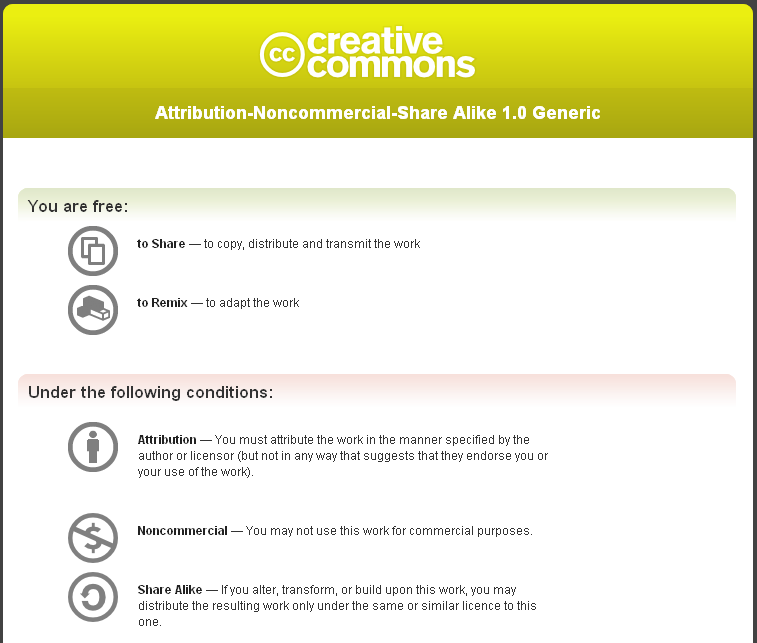
\includegraphics[width=0.65\textwidth]
	{assets/pics/creative_commons.png}
	\caption*{\license}
	\label{fig:lisensi}
\end{figure}

Terkait template ini, gambar lisensi di atas diambil dari \url{http://creativecommons.org/licenses/by-nc-sa/1.0/deed.en_CA}. Jika ingin mengentahui lebih lengkap mengenai \license, silahkan buka \url{http://creativecommons.org/licenses/by-nc-sa/1.0/legalcode}.
Seluruh dokumen yang dibuat dengan menggunakan template ini sepenuhnya menjadi hak milik pembuat dokumen dan bebas didistribusikan sesuai dengan keperluan masing-masing.
Lisensi hanya berlaku jika ada orang yang membuat template baru dengan menggunakan template ini sebagai dasarnya.

Penyusun template ingin berterima kasih kepada Andreas Febrian, Lia Sadita, Fahrurrozi Rahman, Andre Tampubolon, dan Erik Dominikus atas kontribusinya dalam template yang menjadi pendahulu template ini.
Penyusun template juga ingin mengucapkan terima kasih kepada Azhar Kurnia atas kontribusinya dalam template yang menjadi pendahulu template ini.

Semoga template ini dapat membantu orang-orang yang ingin mencoba menggunakan \latex.
Semoga template ini juga tidak berhenti disini dengan ada kontribusi dari para penggunanya.
Jika Anda memiliki perubahan yang dirasa penting untuk disertakan dalam template, silakan lakukan \f{fork} repositori Git template ini di \url{https://gitlab.com/ichlaffterlalu/latex-skripsi-ui-2017}, lalu lakukan \f{merge request} perubahan Anda terhadap \f{branch} \code{master}.
Kami berharap agar \f{template} ini dapat terus diperbarui mengikuti perubahan ketentuan dari pihak Rektorat Universitas Indonesia, dan hal itu tidak mungkin terjadi tanpa kontribusi dari teman-teman sekalian.

% Untuk input gambar tanda tangan, silahkan sesuaikan xshift, yshift, dan width dengan gambar tanda tangan Anda
%\begin{tikzpicture}[remember picture,overlay,shift={(current page.north east)}]
%\node[anchor=north east,xshift=-3cm,yshift=-6.2cm]{
\includegraphics[width=3cm]{assets/pics/tanda_tangan_wikipedia.png}};
%\end{tikzpicture}

\vspace*{0.1cm}
\begin{flushright}
Depok, \tanggalSiapSidang\\[0.1cm]
\ifx\blank\npmDua
	\vspace*{1.5cm}
	\penulisSatu
\else
	Tim Penulis
\fi

\end{flushright}

	\ifodd\thechapterpagecount\forceclearchapter\thispagestyle{onlypage}\fi

	%
	% Lembar Persetujuan Publikasi Ilmiah
	%
	\addChapter{Lembar Persetujuan Karya Ilmiah}
	%
% @author  Andre Tampubolon, Andreas Febrian
% @version 2.2.0
% @edit by Muhammad Aulia Adil Murtito, Ichlasul Affan
%

\chapter*{\uppercase{Halaman Pernyataan Persetujuan Publikasi\\Tugas Akhir untuk Kepentingan Akademis}}
\vspace*{-1cm}
\par\noindent\rule{\textwidth}{3pt}
\vspace*{1cm}
\noindent
Sebagai sivitas akademik Universitas Indonesia,~\ifx\blank\npmDua{saya}\else{kami}\fi~yang bertanda
tangan di bawah ini:

\vspace*{0.2cm}

\pagestyle{onlypage}

\begin{tabular}{p{4.2cm} l p{6.5cm}}
	\ifx\blank\npmDua
	Nama&: & \penulisSatu \\
	NPM&: & \npmSatu \\
	Program Studi&: & \programSatu\\
	\else
	\bo{Penulis 1}\\
	Nama&: & \penulisSatu \\
	NPM&: & \npmSatu \\
	Program Studi&: & \programSatu \vspace*{0.1cm}\\
	\bo{Penulis 2}\\
	Nama&: & \penulisDua \\
	NPM&: & \npmDua \\
	Program Studi&: & \programDua \vspace*{0.1cm}\\
	\fi
	\ifx\blank\npmTiga\else
	\bo{Penulis 3}\\
	Nama&: & \penulisTiga \\
	NPM&: & \npmTiga \\
	Program Studi&: & \programTiga \vspace*{0.1cm}\\
	\fi
	Jenis Karya & : & \type \\
\end{tabular}

\vspace*{0.2cm}

\noindent demi pengembangan ilmu pengetahuan, menyetujui untuk memberikan
kepada Universitas Indonesia \bo{Hak Bebas Royalti Noneksklusif
(\textit{Non-exclusive Royalty Free Right})} atas karya ilmiah~\ifx\blank\npmDua{saya}\else{kami}\fi~yang berjudul:
\begin{center}
	\judul
\end{center}
beserta perangkat yang ada (jika diperlukan). Dengan Hak Bebas Royalti
Noneksklusif ini Universitas Indonesia berhak menyimpan,
mengalihmedia/formatkan, mengelola dalam bentuk pangkalan data
(\textit{database}), merawat, dan memublikasikan tugas akhir~\ifx\blank\npmDua{saya}\else{kami}\fi~selama
tetap mencantumkan nama~\ifx\blank\npmDua{saya}\else{kami}\fi~sebagai penulis/pencipta dan sebagai
pemilik Hak Cipta. \\

\noindent Demikian pernyataan ini~\ifx\blank\npmDua{saya}\else{kami}\fi~buat dengan sebenarnya.

\ifx\blank\npmDua\else\clearpage\fi

% Untuk input gambar tanda tangan, silahkan sesuaikan xshift, yshift, dan width dengan gambar tanda tangan Anda
%\begin{tikzpicture}[remember picture,overlay,shift={(current page.north east)}]
%\node[anchor=north east,xshift=-9cm,yshift=-23.5cm]{
\includegraphics[width=3cm]{assets/pics/tanda_tangan_wikipedia.png}};
%\end{tikzpicture}


\begin{center}
	\vspace*{0.8cm}
	\begin{tabular}{lll}
		Dibuat di&: & Depok \\
		Pada tanggal&: & \tanggalSiapSidang \\
	\end{tabular}\\

	\vspace*{0.2cm}
	Yang menyatakan \\
	\ifx\blank\npmDua
		\vspace*{2cm}
		(\penulisSatu)
	\else
		\begin{multicols}{2}
			Penulis 1:\\
			\vspace*{2cm}
			(\penulisSatu)\\

			Penulis 2:\\
			\vspace*{2cm}
			(\penulisDua)\\
		\end{multicols}
	\fi
	\ifx\blank\npmTiga\else
		\vspace*{0.2cm}
		Penulis 3:\\
		\vspace*{2cm}
		(\penulisTiga)
	\fi
\end{center}

\newpage

	\ifodd\thechapterpagecount\forceclearchapter\thispagestyle{onlypage}\fi
}}


%
% Untuk halaman pertama setiap chapter mulai dari abstrak, tetap berikan mark universitas.
%
\pagestyle{first-pages}


%
% Abstrak
%
\addChapter{Abstrak}
%
% Halaman Abstrak
%
% @author  Andreas Febrian
% @version 2.2.0
% @edit by Ichlasul Affan
%

\chapter*{Abstrak}
\singlespacing

\noindent \begin{tabular}{l l p{10cm}}
	\ifx\blank\npmDua
		Nama&: & \penulisSatu \\
		Program Studi&: & \programSatu \\
	\else
		Nama Penulis 1 / Program Studi&: & \penulisSatu~/ \programSatu\\
		Nama Penulis 2 / Program Studi&: & \penulisDua~/ \programDua\\
	\fi
	\ifx\blank\npmTiga\else
		Nama Penulis 3 / Program Studi&: & \penulisTiga~/ \programTiga\\
	\fi
	Judul&: & \judul \\
	Pembimbing&: & \pembimbingSatu \\
	\ifx\blank\pembimbingDua
    \else
        \ &\ & \pembimbingDua \\
    \fi
    \ifx\blank\pembimbingTiga
    \else
    	\ &\ & \pembimbingTiga \\
    \fi
\end{tabular} \\

\vspace*{0.5cm}

\noindent
Dalam rangka memperkuat integritas akademik pada pembelajaran era digital, penelitian ini mengembangkan sistem deteksi kecurangan yang lebih komprehensif berbasis \textit{machine learning}. Dengan memanfaatkan data log yang kaya dan terstruktur dari Moodle, sistem mengintegrasikan beragam teknik analitik yang mencakup \textbf{deteksi anomali}, \textbf{clustering}, dan \textbf{pembelajaran terawasi} menggunakan model \textit{advanced ensemble}. Berbagai \textit{similarity matrix} (seperti \textit{navigation}, \textit{timing}, dan \textit{answer similarity}) dikombinasikan untuk menghasilkan fitur-fitur baru yang mampu menggali pola perilaku mencurigakan. Selain itu, penerapan \textbf{gradient boosting}, \textbf{neural network}, hingga \textbf{one-class SVM} dan \textbf{ensemble threshold optimization} memberikan kemampuan deteksi kecurangan yang lebih akurat. Hasil evaluasi menunjukkan bahwa metode gabungan ini mampu meningkatkan sensitivitas dan spesifisitas dalam mengungkap potensi kecurangan secara proaktif, sehingga dapat menjadi landasan yang efektif bagi institusi pendidikan dalam mengurangi praktik kecurangan serta memastikan kepatuhan pengguna di platform Moodle.

\vspace*{0.2cm}

\noindent Kata kunci: \\
\f{Moodle, LMS, Log Aktivitas, Pembelajaran Mesin, Deteksi Anomali, Ensemble Methods, Threshold Optimization, Integritas Akademik} \\

\setstretch{1.4}
\newpage


%
% Halaman Abstract
%
% @author  Andreas Febrian
% @version 2.2.0
% @edit by Ichlasul Affan
%

\chapter*{ABSTRACT}
\singlespacing

\noindent \begin{tabular}{l l p{11.0cm}}
	\ifx\blank\npmDua
		Name&: & \penulisSatu \\
		Study Program&: & \studyProgramSatu \\
	\else
		Writer 1 / Study Program&: & \penulisSatu~/ \studyProgramSatu\\
		Writer 2 / Study Program&: & \penulisDua~/ \studyProgramDua\\
	\fi
	\ifx\blank\npmTiga\else
		Writer 3 / Study Program&: & \penulisTiga~/ \studyProgramTiga\\
	\fi
	Title&: & \judulInggris \\
	Counselor&: & \pembimbingSatu \\
	\ifx\blank\pembimbingDua
    \else
        \ &\ & \pembimbingDua \\
    \fi
    \ifx\blank\pembimbingTiga
    \else
    	\ &\ & \pembimbingTiga \\
    \fi
\end{tabular} \\

\vspace*{0.5cm}

\noindent
In order to strengthen academic integrity in the digital learning era, this study develops a more comprehensive cheating detection system based on machine learning. By utilizing rich and structured log data from Moodle, our system integrates multiple analytical techniques including anomaly detection, clustering, and supervised learning through advanced ensemble models. Various similarity matrices (such as navigation, timing, and answer similarity) are combined to generate new features that uncover potentially suspicious behavior patterns. In addition, the application of gradient boosting, neural network, one-class SVM, and ensemble threshold optimization provides more accurate cheating detection capabilities. Evaluation results show that this combined method enhances both sensitivity and specificity in proactively revealing potential cheating incidents, making it an effective foundation for educational institutions to minimize dishonest practices and ensure user compliance within the Moodle platform.

\vspace*{0.2cm}

\noindent Key words: \\
Moodle, LMS, Activity Logs, Machine Learning, Anomaly Detection, Ensemble Methods, Threshold Optimization, Academic Integrity \\

\setstretch{1.4}
\newpage



%
% Daftar Isi, Gambar, dan Tabel
%

\addDefaultListPage{\tableofcontents}
\addDefaultListPage{\listoffigures}
\addDefaultListPage{\listoftables}


%
% Daftar Kode Program
% Jika tidak digunakan, commment kode ini.
%
\addCustomListPage{\listoflistings}{\lstlistlistingname}


%
% Daftar Equation (Persamaan Matematis)
% Jika bagian ini diperlukan, uncomment kode ini.
%
% \addCustomListPage{\listofequ}{\listofequname}


%
% Daftar Isi yang Didefinisikan Sendiri (Custom)
% Definisi jenis objek baru dapat dilakukan di uithesis.sty
%
% \addCustomListPage{\listofthing}{\listofthingname}


%
% Daftar Lampiran
% Jika tidak digunakan, commment kode ini.
%
%\addCustomListPage{\listofappendix}{\listofappendixname}


% Kembalikan pengaturan chapter dan daftar isi ke aturan awal mulai dari halaman ini
\noCAPinToC
\ifodd\thechapterpagecount\clearpage\else\forceclearchapter\fi

% Jika penomoran romawi selesai di ganjil
% \naiveoddclearchapter
% Jika penomoran romawi selesai di genap
% \naiveevenclearchapter


%
% Gunakan penomoran Arab (1, 2, 3, ...) setelah bagian ini.
%
\pagenumbering{arabic}
\pagestyle{standard}


%
% Isi dari Tugas Akhir/Karya Ilmiah
%
\setoddevenheader
%-----------------------------------------------------------------------------%
\chapter{\babSatu}
\label{bab:1}
%-----------------------------------------------------------------------------%
Pada bab ini, akan dijelaskan tentang topik penelitian, termasuk di dalamnya latar belakang dan permasalahan yang diselesaikan pada penelitian ini. 

%-----------------------------------------------------------------------------%
\section{Latar Belakang}
\label{sec:latarBelakang}
%-----------------------------------------------------------------------------%

Era digital mendorong transformasi pendidikan tinggi secara pesat, terutama sejak pandemi COVID-19. Institusi perguruan tinggi berbondong-bondong mengadopsi \textit{Learning Management System} (LMS) seperti Moodle untuk mendukung pembelajaran daring dan pelaksanaan ujian jarak jauh \cite{Yulita2023}. Digitalisasi ini membawa manfaat dalam hal fleksibilitas dan jangkauan, namun juga menimbulkan tantangan baru terhadap integritas akademik. Menjaga kejujuran akademik di lingkungan pembelajaran daring kini menjadi isu krusial, karena proses evaluasi yang berpindah ke ranah online rentan disalahgunakan untuk melakukan kecurangan \cite{Kamalov2021}.

Studi menunjukkan bahwa risiko kecurangan akademik cenderung meningkat dalam konteks pembelajaran daring. Lanier menemukan tingkat kecurangan yang jauh lebih tinggi pada kelas jarak jauh dibanding kelas tatap muka tradisional \cite{Lanier2006}. Sementara itu, survei terhadap mahasiswa dan dosen di Norwegia mengidentifikasi enam modus kecurangan paling umum dalam ujian daring, seperti peniruan identitas, penggunaan bahan terlarang, dan kolaborasi tidak sah \cite{Chirumamilla2020}.

Dalam konteks ini, data log aktivitas Moodle menjadi sumber informasi yang sangat berharga. Moodle secara otomatis merekam jejak interaksi pengguna secara terstruktur, mencakup waktu akses, pola navigasi, durasi pengerjaan soal, hingga kesamaan jawaban antar peserta. Analisis mendalam terhadap log ini berpotensi mengungkap berbagai pola perilaku yang mengindikasikan kecurangan, seperti kolaborasi tidak sah yang terdeteksi dari kesamaan pola navigasi dan jawaban \cite{Murdoch2019}, serta berbagai anomali perilaku selama pandemi \cite{Balderas2020}.

Pendekatan konvensional untuk mendeteksi kecurangan umumnya mengandalkan pemeriksaan manual atau sistem berbasis aturan sederhana. Namun, metode ini memiliki keterbatasan serius, seperti skalabilitas rendah dan kecenderungan menghasilkan \textit{false positives} \cite{MorenoMarcos2023}. 

Sebagai solusi, penelitian ini mengusulkan pendekatan berbasis \textit{machine learning} yang mengintegrasikan beragam teknik analitik. Kerangka kerja yang dikembangkan berfokus pada model pembelajaran terawasi (\textit{supervised learning}) seperti \textit{Gradient Boosting}, \textit{Random Forest}, dan \textit{Neural Network}, yang diperkuat dengan metode deteksi anomali seperti \textit{Isolation Forest} dan \textit{Local Outlier Factor} sebagai teknik komplementer. Pendekatan ensemble ini dilengkapi dengan analisis matriks kesamaan (\textit{similarity matrices}) yang mencakup pola navigasi, waktu pengerjaan, dan jawaban mahasiswa, serta optimasi ambang batas (\textit{threshold optimization}) untuk meningkatkan akurasi deteksi.

Integrasi berbagai teknik ini memungkinkan sistem mengenali pola-pola mencurigakan dengan lebih akurat, seperti yang ditunjukkan dalam penelitian sebelumnya menggunakan data MOOC \cite{Alexandron2019}. Penggunaan matriks kesamaan dan analisis graf juga terbukti efektif dalam mengungkap kolusi antar mahasiswa \cite{Chang2023}. Dengan demikian, penelitian ini berkontribusi pada pengembangan sistem deteksi kecurangan yang lebih komprehensif dan adaptif untuk platform Moodle.

%-----------------------------------------------------------------------------%
\section{Permasalahan}
\label{sec:masalah}
%-----------------------------------------------------------------------------%

Kecurangan akademik merupakan permasalahan serius di institusi pendidikan tinggi karena dapat merusak integritas dan kualitas hasil pembelajaran. Dalam konteks pembelajaran \textit{e-learning} menggunakan platform Moodle, potensi terjadinya kecurangan akademik semakin tinggi seiring dengan meningkatnya penggunaan ujian daring dan tugas online. Beragam bentuk kecurangan dapat terjadi, misalnya kolusi antar mahasiswa untuk berbagi jawaban, penyalahgunaan akun, atau penggunaan sumber tidak sah selama ujian.

Kompleksitas permasalahan ini menuntut pendekatan deteksi yang lebih canggih, yang tidak hanya mengandalkan satu metode, melainkan mengintegrasikan berbagai teknik analitik untuk menghasilkan deteksi yang lebih akurat dan dapat diandalkan. Diperlukan juga kemampuan untuk menganalisis berbagai aspek perilaku pengguna secara simultan, dari pola navigasi hingga kesamaan jawaban, serta mengoptimalkan parameter deteksi untuk meminimalkan kesalahan klasifikasi.

%-----------------------------------------------------------------------------%
\subsection{Pertanyaan Penelitian}
\label{sec:definisiMasalah}
%-----------------------------------------------------------------------------%
Berdasarkan permasalahan yang telah diuraikan, penelitian ini berusaha menjawab pertanyaan-pertanyaan berikut:
\begin{enumerate}
    \item Bagaimana mengembangkan pendekatan berbasis pembelajaran mesin yang efektif untuk mendeteksi potensi kecurangan akademik dalam pembelajaran daring menggunakan data log aktivitas Moodle?
    \item Sejauh mana integrasi berbagai teknik analisis data dapat meningkatkan akurasi dan reliabilitas deteksi perilaku mencurigakan dalam konteks pembelajaran daring?
    \item Bagaimana karakteristik dan pola perilaku pengguna yang teridentifikasi dari hasil analisis dapat memberikan wawasan untuk meningkatkan integritas akademik dalam pembelajaran daring?
\end{enumerate}

%-----------------------------------------------------------------------------%
\subsection{Batasan Penelitian}
\label{sec:batasanMasalah}
%-----------------------------------------------------------------------------%
Untuk memastikan penelitian ini tetap terfokus dan terarah, beberapa batasan dan ruang lingkup berikut diterapkan:
\begin{enumerate}
    \item Lingkup Data: Data yang digunakan dalam penelitian ini dibatasi pada log aktivitas pengguna dari platform Moodle di lingkungan Fasilkom UI,dengan model dilatih menggunakan data artifisial yang karakteristiknya divalidasi terhadap data riil, dan kemudian diterapkan pada data log riil Fasilkom UI untuk analisis.
    \item Jenis Kecurangan: Deteksi difokuskan pada pola perilaku mencurigakan yang tercermin dalam log aktivitas, matriks kesamaan, dan interaksi antar pengguna.
    \item Metode dan Algoritma: Pendekatan utama menggunakan model pembelajaran terawasi dengan ensemble, didukung metode deteksi anomali sebagai komplemen.
    \item Mode Implementasi: Sistem deteksi diimplementasikan dalam modus \textit{offline} untuk analisis retrospektif.
    \item Evaluasi: Kinerja sistem dievaluasi menggunakan metrik standar seperti presisi, sensitivitas, dan skor F1.
\end{enumerate}

%-----------------------------------------------------------------------------%
\section{Tujuan Penelitian}
\label{sec:tujuan}
%-----------------------------------------------------------------------------%
Penelitian ini memiliki tujuan utama untuk mengembangkan sistem deteksi kecurangan yang komprehensif berbasis analisis log aktivitas Moodle. Secara terperinci, tujuan penelitian ini adalah:
\begin{enumerate}
    \item Merancang dan mengimplementasikan kerangka kerja deteksi yang mengintegrasikan model pembelajaran terawasi dengan ensemble, didukung metode deteksi anomali, analisis matriks kesamaan, dan optimasi ambang batas.
    \item Mengembangkan dan mengevaluasi fitur-fitur baru berbasis matriks kesamaan untuk meningkatkan akurasi deteksi.
    \item Melakukan pengujian menyeluruh terhadap kinerja sistem menggunakan data log Moodle Fasilkom UI.
    \item Menganalisis dan menginterpretasikan pola-pola perilaku mencurigakan yang terdeteksi untuk mendukung upaya pencegahan kecurangan.
\end{enumerate}

%-----------------------------------------------------------------------------%
\section{Manfaat Penelitian}
\label{sec:manfaat}
%-----------------------------------------------------------------------------%
Penelitian ini diharapkan memberikan manfaat baik secara teoretis maupun praktis:
\begin{enumerate}
    \item Manfaat Teoretis:
    \begin{enumerate}
        \item Kontribusi pada pengembangan metode deteksi kecurangan berbasis ensemble.
        \item Pemahaman baru tentang efektivitas matriks kesamaan dalam analisis perilaku.
        \item Landasan metodologis untuk penelitian lanjutan.
    \end{enumerate}
    
    \item Manfaat Praktis:
    \begin{enumerate}
        \item Sistem deteksi dini yang lebih akurat untuk institusi pendidikan.
        \item Dukungan objektif untuk pengambilan keputusan terkait integritas akademik.
        \item Peningkatan efektivitas monitoring pembelajaran daring.
        \item Dasar pengembangan sistem deteksi real-time di masa depan.
    \end{enumerate}
\end{enumerate}

%-----------------------------------------------------------------------------%
\section{Langkah Penelitian}
\label{sec:langkahPenelitian}
%-----------------------------------------------------------------------------%

Berikut ini adalah langkah penelitian yang dilakukan:

\begin{enumerate}
\item \textbf{Tinjauan Literatur}\\
Mengkaji teori dan penelitian terkait deteksi kecurangan, metode ensemble, dan analisis matriks kesamaan dalam konteks pembelajaran daring.

\item \textbf{Pengumpulan dan Pengolahan Data}\\
Mengumpulkan log aktivitas Moodle, melakukan pembersihan data, dan mengekstraksi fitur-fitur relevan termasuk matriks kesamaan.

\item \textbf{Pengembangan Sistem}\\
Mengimplementasikan kerangka kerja deteksi yang mengintegrasikan model pembelajaran terawasi (\textit{Gradient Boosting}, \textit{Random Forest}, \textit{Neural Network}) sebagai komponen utama, diperkaya dengan metode deteksi anomali, analisis matriks kesamaan, dan optimasi ambang batas.

\item \textbf{Evaluasi dan Analisis}\\
Menguji kinerja sistem menggunakan metrik standar, menganalisis pola-pola yang terdeteksi, dan menginterpretasikan implikasinya.

\item \textbf{Penarikan Kesimpulan}\\
Menyimpulkan efektivitas pendekatan yang diusulkan dan merumuskan rekomendasi untuk pengembangan sistem dan penelitian lanjutan.
\end{enumerate}

%-----------------------------------------------------------------------------%
\section{Sistematika Penulisan}
\label{sec:sistematikaPenulisan}
%-----------------------------------------------------------------------------%

Sistematika penulisan laporan penelitian ini adalah sebagai berikut:

\begin{itemize}
\item \textbf{Bab 1 Pendahuluan}\\
Berisi latar belakang penelitian, perumusan masalah, batasan penelitian, tujuan penelitian, manfaat penelitian, langkah-langkah penelitian, serta sistematika penulisan.

\item \textbf{Bab 2 Landasan Teori dan Studi Literatur}\\
Mengkaji konsep-konsep fundamental tentang integritas akademik dalam pembelajaran daring, teknik-teknik pembelajaran mesin untuk deteksi anomali, serta penelitian-penelitian terkait dalam bidang analisis perilaku pengguna sistem pembelajaran daring.

\item \textbf{Bab 3 Metodologi dan Rancangan Sistem}\\
Menjelaskan pendekatan metodologis yang digunakan, termasuk desain sistem deteksi, proses pengolahan data, pemilihan dan integrasi metode analisis, serta kerangka evaluasi yang diterapkan.

\item \textbf{Bab 4 Implementasi dan Hasil Eksperimen}\\
Memaparkan implementasi sistem yang dikembangkan, hasil eksperimen yang dilakukan, serta analisis kinerja berdasarkan berbagai metrik evaluasi.

\item \textbf{Bab 5 Analisis dan Pembahasan}\\
Menganalisis secara mendalam temuan-temuan penelitian, interpretasi pola perilaku yang terdeteksi, serta implikasinya terhadap praktik pembelajaran daring.

\item \textbf{Bab 6 Kesimpulan dan Saran}\\
Menyajikan kesimpulan penelitian, kontribusi yang dihasilkan, keterbatasan yang ditemui, serta rekomendasi untuk pengembangan dan penelitian lanjutan.
\end{itemize}


\clearchapter
%-----------------------------------------------------------------------------%
\chapter{\babDua}
\label{bab:2}
%-----------------------------------------------------------------------------%

Bab ini menyajikan tinjauan pustaka yang komprehensif mengenai landasan teoretis dan penelitian terkait sistem deteksi kecurangan akademik berbasis kecerdasan buatan. Pembahasan mencakup evolusi masalah integritas akademik dalam pembelajaran daring, perkembangan teknik \textit{machine learning} untuk deteksi anomali, serta aplikasi spesifik dalam lingkungan \textit{Learning Management System} (LMS) seperti Moodle.

%-----------------------------------------------------------------------------%
\section{Integritas Akademik dalam Era Pembelajaran Daring}
\label{sec:integritasAkademik}
%-----------------------------------------------------------------------------%

\subsection{Evolusi Tantangan Integritas Akademik}
\label{subsec:evolusiTantangan}

Integritas akademik telah menjadi perhatian fundamental dalam dunia pendidikan sejak lama, namun transformasi digital pendidikan telah mengubah secara signifikan lanskap dan karakteristik permasalahan ini. Lanier \cite{Lanier2006} dalam penelitiannya yang menjadi rujukan penting, menemukan bahwa tingkat kecurangan dalam pembelajaran jarak jauh cenderung lebih tinggi dibandingkan dengan kelas tatap muka tradisional. Temuan ini menjadi dasar pemahaman bahwa lingkungan pembelajaran daring memerlukan pendekatan pemantauan yang berbeda dan lebih komprehensif.

Chirumamilla dkk. \cite{Chirumamilla2020} melalui survei terhadap mahasiswa dan dosen di Norwegia, mengidentifikasi enam modus kecurangan paling umum dalam ujian daring: (1) peniruan identitas (\textit{identity theft}), (2) penggunaan bahan bantuan terlarang, (3) kolaborasi tidak sah antarpeserta, (4) penggunaan perangkat komunikasi selama ujian, (5) akses ke sumber eksternal tanpa izin, dan (6) manipulasi waktu pengerjaan. Klasifikasi ini memberikan kerangka pemahaman yang sistematis tentang berbagai bentuk pelanggaran yang perlu dideteksi oleh sistem otomatis.

Penelitian terbaru menunjukkan bahwa pandemi COVID-19 telah mempercepat adopsi pembelajaran daring sekaligus meningkatkan kompleksitas permasalahan integritas akademik. Yulita dkk. \cite{Yulita2023} mengamati peningkatan signifikan dalam kecanggihan metode kecurangan, termasuk penggunaan teknologi untuk memfasilitasi kolusi dan berbagi informasi secara real-time selama ujian berlangsung.

\subsection{Karakteristik Kecurangan dalam Lingkungan Digital}

Lingkungan pembelajaran digital memiliki karakteristik unik yang membedakannya dari pengaturan tradisional. Murdoch dan House \cite{Murdoch2019} mengidentifikasi fenomena \textit{"ghost in the shell"}, yaitu perpaduan antara kecurangan berbasis kontrak (\textit{contract cheating}) dengan peniruan identitas daring. Fenomena ini menunjukkan evolusi kecurangan dari tindakan individual menjadi operasi yang lebih terorganisasi dan teknologis.

Balderas dan Caballero-Hern\'{a}ndez \cite{Balderas2020} dalam analisis mereka terhadap rekam jejak pembelajaran selama pandemi, menemukan bahwa pola perilaku mencurigakan dapat diidentifikasi melalui analisis temporal dan spasial aktivitas mahasiswa. Temuan ini memperkuat argumen bahwa data log aktivitas mengandung informasi yang kaya untuk deteksi kecurangan, asalkan dianalisis dengan metode yang tepat.

%-----------------------------------------------------------------------------%
\section{Pendekatan \textit{Machine Learning} untuk Deteksi Kecurangan}
\label{sec:mlApproaches}
%-----------------------------------------------------------------------------%

\subsection{Evolusi dari Sistem Berbasis Aturan ke \textit{Machine Learning}}

Pendekatan tradisional untuk deteksi kecurangan akademik umumnya mengandalkan sistem berbasis aturan (\textit{rule-based systems}) yang menggunakan ambang batas statis untuk mengidentifikasi perilaku mencurigakan. Huda dkk. \cite{article:rule_based_limitations} mengidentifikasi beberapa keterbatasan fundamental dari pendekatan ini: (1) rendahnya akurasi dalam menangani pola perilaku yang kompleks, (2) tingginya tingkat \textit{false positive} yang mengakibatkan banyak mahasiswa normal yang salah dituduh, (3) ketidakmampuan untuk beradaptasi dengan modus kecurangan yang berkembang, dan (4) kesulitan dalam menangani variasi kontekstual antarmata kuliah atau institusi.

Sebagai respons terhadap keterbatasan ini, penelitian modern beralih ke pendekatan berbasis \textit{machine learning} yang menawarkan kemampuan adaptif dan akurasi yang lebih tinggi. Kamalov dkk. \cite{Kamalov2021} menunjukkan bahwa model pembelajaran mesin dapat mencapai akurasi deteksi hingga 94\% dalam mengidentifikasi kecurangan ujian, jauh melampaui kinerja sistem berbasis aturan tradisional.

\subsection{Teknik \textit{Supervised Learning} untuk Deteksi Kecurangan}

Pendekatan pembelajaran terawasi (\textit{supervised learning}) telah menjadi metode dominan dalam deteksi kecurangan akademik karena kemampuannya dalam mempelajari pola dari data berlabel. Zhou dan Jiao \cite{Zhou2022} dalam penelitian mereka tentang augmentasi data untuk deteksi kecurangan dalam asesmen skala besar, mendemonstrasikan efektivitas berbagai algoritma pembelajaran terawasi, termasuk \textit{Random Forest}, \textit{Support Vector Machine}, dan \textit{Gradient Boosting}.

Alsabhan \cite{Alsabhan2023} mengembangkan pendekatan hibrida yang mengintegrasikan \textit{Long Short-Term Memory} (LSTM) dengan teknik pembelajaran mesin tradisional untuk mendeteksi kecurangan mahasiswa di perguruan tinggi. Penelitian ini menunjukkan bahwa kombinasi neural network dengan algoritma ensemble dapat meningkatkan akurasi deteksi hingga 96,8\%, dengan kemampuan khusus dalam menangkap pola temporal yang kompleks dalam perilaku mahasiswa.

Chang dan Chang \cite{Chang2023} melakukan studi komprehensif tentang deteksi kolusi dalam ujian, dengan fokus pada teknik pembelajaran mesin dan representasi fitur. Mereka menemukan bahwa \textit{feature engineering} yang tepat, terutama yang berkaitan dengan matriks kesamaan dan analisis graf, dapat secara signifikan meningkatkan kemampuan deteksi kolaborasi tidak sah antarpeserta ujian.

\subsection{Deteksi Anomali dan \textit{Unsupervised Learning}}

Meskipun pembelajaran terawasi menunjukkan kinerja yang baik, ketersediaan data berlabel yang berkualitas seringkali menjadi kendala dalam implementasi praktis. Sebagai alternatif, pendekatan deteksi anomali berbasis \textit{unsupervised learning} menawarkan solusi yang menjanjikan. Cen dkk. \cite{survey:anomaly_detection_edu} mengembangkan kerangka kerja untuk deteksi anomali tanpa pengawasan dalam sistem \textit{e-learning}, yang mampu mengidentifikasi pola perilaku yang tidak biasa tanpa memerlukan data berlabel sebelumnya.

Alexandron dkk. \cite{Alexandron2019} mengusulkan metode deteksi anomali tujuan umum untuk mengidentifikasi kecurangan dalam \textit{Massive Open Online Courses} (MOOC). Penelitian mereka menunjukkan bahwa teknik deteksi anomali seperti \textit{Isolation Forest} dan \textit{Local Outlier Factor} dapat efektif dalam mengidentifikasi pola perilaku yang menyimpang dari norma, dengan tingkat presisi yang dapat diterima untuk implementasi praktis.

%-----------------------------------------------------------------------------%
\section{Sistem Deteksi Khusus Platform Moodle}
\label{sec:moodleSpecific}
%-----------------------------------------------------------------------------%

\subsection{Karakteristik Data Log Moodle}

Moodle sebagai salah satu LMS yang paling banyak digunakan di dunia, menyediakan sistem pencatatan log yang komprehensif dan terstruktur. Mazza dan Dimitrova \cite{article:moodle_logs} dalam penelitian pionir mereka, menjelaskan bahwa log aktivitas Moodle mengandung informasi detail tentang setiap interaksi pengguna dengan platform, termasuk timestamp, tipe aktivitas, durasi, dan konteks akademik.

Data log Moodle memiliki beberapa karakteristik unik yang membuatnya sangat cocok untuk analisis \textit{machine learning}: (1) granularitas tinggi dalam perekaman aktivitas, (2) konsistensi format data lintas berbagai modul, (3) integrasi dengan konteks pembelajaran yang memungkinkan analisis berbasis mata kuliah, dan (4) kemampuan pelacakan yang mencakup tidak hanya aktivitas ujian tetapi juga pola belajar secara keseluruhan.

\subsection{Implementasi Sistem Deteksi Terintegrasi}

Shatnawi dkk. \cite{Shatnawi2024} mengembangkan sistem deteksi kecurangan ujian elektronik yang terintegrasi langsung dengan platform Moodle LMS. Sistem ini menggunakan pendekatan pembelajaran mesin dengan metode statistik yang mampu mencapai akurasi 100\% dalam mendeteksi berbagai jenis anomali, termasuk deteksi waktu respons yang tidak wajar, pola navigasi mencurigakan, dan aktivitas yang tidak konsisten dengan perilaku normal mahasiswa.

Moreno-Marcos dkk. \cite{MorenoMarcos2023} mengembangkan Statoodle, sebuah alat \textit{learning analytics} yang diintegrasikan langsung dengan Moodle untuk menganalisis aksi mahasiswa dan mencegah kecurangan. Sistem ini menggunakan pendekatan pemantauan waktu nyata yang dapat memberikan peringatan dini kepada pengawas ujian ketika terdeteksi aktivitas mencurigakan.

Pendekatan terintegrasi ini menawarkan beberapa keuntungan: (1) akses langsung ke data log tanpa perlu ekspor manual, (2) kemampuan pemantauan waktu nyata, (3) integrasi dengan alur kerja yang ada di institusi pendidikan, dan (4) kemudahan dalam implementasi tindakan preventif atau responsif.

\subsection{Analisis Kesamaan dan Deteksi Kolusi}

Salah satu kekuatan utama platform Moodle adalah kemampuannya dalam menyediakan data yang memungkinkan analisis kesamaan antarpeserta. Chang dan Chang \cite{Chang2023} menunjukkan bahwa analisis matriks kesamaan berbasis jawaban, pola navigasi, dan waktu dapat secara efektif mengidentifikasi kolusi antarmahasiswa.

Teknik analisis graf juga dapat diterapkan pada data Moodle untuk mengidentifikasi kluster mahasiswa yang menunjukkan pola perilaku yang serupa secara tidak wajar. Pendekatan ini tidak hanya dapat mendeteksi kecurangan individual, tetapi juga mengungkap jaringan kolaborasi yang lebih luas.

%-----------------------------------------------------------------------------%
\section{\textit{Learning Analytics} dan \textit{Educational Data Mining}}
\label{sec:learningAnalytics}
%-----------------------------------------------------------------------------%

\subsection{Evolusi \textit{Learning Analytics} sebagai Disiplin}

\textit{Learning analytics} telah berkembang menjadi disiplin yang matang dalam dekade terakhir, dengan fokus pada penggunaan data pendidikan untuk meningkatkan proses dan hasil pembelajaran. Siemens dan Long (2011) mendefinisikan \textit{learning analytics} sebagai pengukuran, pengumpulan, analisis, dan pelaporan data tentang pelajar dan konteks mereka, dengan tujuan memahami dan mengoptimalkan pembelajaran serta lingkungan tempat pembelajaran tersebut terjadi.

Dalam konteks deteksi kecurangan, \textit{learning analytics} menyediakan kerangka metodologis dan teknologis yang komprehensif. Ferguson (2012) mengidentifikasi bahwa pendekatan \textit{learning analytics} tidak hanya fokus pada deteksi masalah, tetapi juga pada pemahaman mendalam tentang pola perilaku belajar yang dapat membantu dalam pencegahan proaktif.

\subsection{Aplikasi \textit{Educational Data Mining} untuk Deteksi Anomali}

\textit{Educational Data Mining} (EDM) sebagai subbidang dari \textit{learning analytics} menyediakan teknik-teknik khusus untuk ekstraksi pola dari data pendidikan. Romero dan Ventura (2020) dalam ulasan komprehensif mereka, mengidentifikasi bahwa teknik EDM telah berkembang dari analisis deskriptif sederhana menjadi model prediktif yang kompleks.

Dalam konteks deteksi kecurangan, EDM menawarkan beberapa teknik yang relevan: (1) \textit{sequence mining} untuk menganalisis pola navigasi, (2) \textit{clustering} untuk mengidentifikasi grup mahasiswa dengan perilaku serupa, (3) \textit{association rule mining} untuk menemukan hubungan antaraktivitas, dan (4) \textit{classification} untuk membedakan perilaku normal dan mencurigakan.

\subsection{Integrasi Perspektif Pedagogis dan Teknologis}

Aspek penting dalam pengembangan sistem deteksi kecurangan adalah integrasi antara perspektif pedagogis dan teknologis. Ga\v{s}evi\'{c} dkk. (2015) menekankan bahwa sistem \textit{learning analytics} yang efektif harus mempertimbangkan tidak hanya aspek teknis deteksi, tetapi juga implikasi pedagogis dan etis dari implementasi sistem tersebut.

Dalam konteks deteksi kecurangan, hal ini berarti sistem harus dirancang tidak hanya untuk mengidentifikasi pelanggaran, tetapi juga untuk mendukung proses pembelajaran yang adil dan mendorong integritas akademik melalui pendekatan yang konstruktif daripada sekadar bersifat hukuman.

%-----------------------------------------------------------------------------%
\section{Teknik Ensemble dan Optimasi Model}
\label{sec:ensembleTechniques}
%-----------------------------------------------------------------------------%

\subsection{Pendekatan \textit{Ensemble Learning}}

\textit{Ensemble learning} telah terbukti sebagai salah satu pendekatan paling efektif dalam meningkatkan akurasi dan ketahanan model \textit{machine learning}. Dalam konteks deteksi kecurangan akademik, teknik ensemble menawarkan keuntungan khusus karena kemampuannya dalam menggabungkan kekuatan berbagai algoritma untuk menangani kompleksitas dan variasi pola kecurangan.

Zhou (2012) dalam "Ensemble Methods: Foundations and Algorithms" menjelaskan bahwa kekuatan ensemble terletak pada prinsip "diversity and accuracy", yaitu kombinasi model yang beragam namun akurat dapat menghasilkan kinerja yang superior dibandingkan model individual. Dalam konteks deteksi kecurangan, keberagaman ini sangat penting karena berbagai jenis kecurangan mungkin lebih baik dideteksi oleh algoritma yang berbeda.

\subsection{Strategi Integrasi Multialgoritma}

Penelitian terkini menunjukkan bahwa integrasi strategis antara model pembelajaran terawasi dengan teknik deteksi anomali dapat menghasilkan sistem yang lebih kuat. Nadeem dkk. \cite{Nadeem2024} dalam penelitian mereka tentang teknik pembelajaran mesin canggih untuk deteksi penipuan keuangan, menunjukkan bahwa kombinasi supervised dan unsupervised learning dapat mengatasi keterbatasan masing-masing pendekatan: supervised learning memberikan akurasi tinggi pada pola yang dikenal, sementara unsupervised learning dapat mendeteksi anomali baru yang belum pernah ditemui sebelumnya.

Dalam implementasi praktis, strategi ensemble dapat mencakup: (1) \textit{voting classifiers} yang menggabungkan prediksi beberapa model, (2) \textit{stacking} yang menggunakan meta-learner untuk mengoptimalkan kombinasi, (3) \textit{bagging} untuk mengurangi varians, dan (4) \textit{boosting} untuk mengurangi bias.

\subsection{Optimasi Ambang Batas dan Hiperparameter}

Optimasi ambang batas merupakan aspek kritis dalam sistem deteksi kecurangan karena pertukaran antara false positive dan false negative memiliki implikasi praktis yang signifikan. Ambang batas yang terlalu rendah akan menghasilkan banyak false positive yang dapat merugikan mahasiswa yang tidak bersalah, sementara ambang batas yang terlalu tinggi dapat membiarkan kecurangan lolos dari deteksi.

Niu dkk. \cite{Niu2025} dalam ulasan sistematis tentang metodologi pembelajaran mesin yang efektif menunjukkan bahwa optimasi ambang batas sebaiknya dilakukan dengan mempertimbangkan cost-sensitive learning, yaitu \textit{cost} dari berbagai jenis kesalahan diperhitungkan secara eksplisit. Dalam konteks akademik, \textit{cost} dari false positive (menuduh mahasiswa yang tidak bersalah) mungkin berbeda dengan \textit{cost} dari false negative (membiarkan pelanggar akademik lolos).

%-----------------------------------------------------------------------------%
\section{Analisis Matriks Kesamaan dan \textit{Graph-Based Detection}}
\label{sec:similarityAnalysis}
%-----------------------------------------------------------------------------%

\subsection{Teori Matriks Kesamaan dalam Deteksi Kolusi}

Analisis matriks kesamaan telah menjadi teknik fundamental dalam deteksi kolaborasi tidak sah dalam konteks akademik. Konsep ini didasarkan pada premis bahwa mahasiswa yang melakukan kolusi akan menunjukkan pola perilaku yang tidak natural serupa, baik dalam hal jawaban, pola navigasi, maupun waktu.

Ukuran kesamaan yang umum digunakan dalam konteks ini meliputi: (1) \textit{Cosine similarity} untuk mengukur kemiripan vektor fitur, (2) \textit{Jaccard similarity} untuk data kategorikal, (3) \textit{Pearson correlation} untuk hubungan linear, dan (4) \textit{Edit distance} untuk data sekuensial. Pemilihan ukuran yang tepat sangat bergantung pada jenis data dan karakteristik kecurangan yang ingin dideteksi.

\subsection{Analisis Graf dan \textit{Network Detection}}

Pendekatan berbasis graf menawarkan perspektif yang kuat untuk memahami pola kolaborasi dalam skala yang lebih besar. Dalam representasi graf, mahasiswa dapat dimodelkan sebagai simpul, sementara sisi merepresentasikan tingkat kesamaan atau kolaborasi yang dicurigai.

Teknik analisis graf yang relevan meliputi: (1) \textit{community detection} untuk mengidentifikasi kluster mahasiswa yang berkolaborasi, (2) \textit{centrality measures} untuk mengidentifikasi individu yang menjadi pusat dalam jaringan kolaborasi, (3) \textit{clustering coefficient} untuk mengukur tingkat interkoneksi, dan (4) \textit{modularity analysis} untuk memvalidasi struktur komunitas.

\subsection{Analisis Temporal dan \textit{Dynamic Networks}}

Aspek temporal dalam analisis kesamaan memberikan dimensi tambahan yang penting. Kecurangan seringkali menunjukkan pola temporal yang karakteristik, seperti pengiriman jawaban secara bersamaan, pola navigasi yang sinkron, atau perubahan jawaban yang terkoordinasi.

Analisis jaringan dinamis dapat mengungkap pola kolaborasi yang berkembang selama ujian berlangsung, memberikan wawasan yang tidak dapat diperoleh dari analisis statis. Hal ini sangat relevan untuk ujian yang berlangsung dalam periode waktu yang diperpanjang atau untuk menganalisis pola kecurangan lintas beberapa sesi.

%-----------------------------------------------------------------------------%
\section{Evaluasi dan Validasi Sistem Deteksi}
\label{sec:evaluationValidation}
%-----------------------------------------------------------------------------%

\subsection{Metrik Evaluasi dalam Konteks Akademik}

Evaluasi sistem deteksi kecurangan memerlukan pertimbangan khusus karena karakteristik unik dari domain akademik. Metrik evaluasi standar seperti akurasi, presisi, recall, dan F1-score tetap relevan, namun interpretasi dan prioritas mereka harus disesuaikan dengan konteks.

Dalam pengaturan akademik, false positive (menuduh mahasiswa yang tidak bersalah) memiliki implikasi yang sangat serius, termasuk kerusakan reputasi, stres psikologis, dan konsekuensi hukum yang potensial. Oleh karena itu, presisi menjadi metrik yang sangat kritis. Di sisi lain, false negative (membiarkan pelanggar akademik lolos) dapat merusak keadilan sistem evaluasi dan mengancam integritas akademik secara keseluruhan.

\subsection{Validasi Lintas Domain dan Generalisasi}

Salah satu tantangan utama dalam pengembangan sistem deteksi kecurangan adalah memastikan generalisasi lintas mata kuliah, institusi, dan konteks yang berbeda. Model yang dilatih pada satu set data mungkin tidak berkinerja baik pada konteks yang berbeda karena variasi dalam perilaku mahasiswa, struktur mata kuliah, atau format ujian.

Strategi validasi silang yang kuat perlu mempertimbangkan tidak hanya pembagian acak, tetapi juga stratifikasi berdasarkan jenis mata kuliah, tingkat mahasiswa, atau faktor temporal. Hal ini penting untuk memastikan bahwa model dapat menggeneralisasi ke situasi dunia nyata yang beragam.

\subsection{Aspek Etis dan Keadilan}

Implementasi sistem deteksi kecurangan otomatis menimbulkan berbagai pertanyaan etis yang perlu dipertimbangkan secara serius. Keadilan algoritma menjadi isu yang kritis, terutama terkait dengan bias potensial terhadap kelompok mahasiswa tertentu.

Aspek etis yang perlu dipertimbangkan meliputi: (1) transparansi dalam proses pengambilan keputusan, (2) dapat dijelaskannya prediksi yang dihasilkan, (3) keadilan lintas kelompok demografis yang berbeda, (4) perlindungan privasi dalam penanganan data, dan (5) pengawasan manusia dalam proses pengambilan keputusan final.

%-----------------------------------------------------------------------------%
\section{Kesenjangan Penelitian dan Peluang Pengembangan}
\label{sec:researchGaps}
%-----------------------------------------------------------------------------%

\subsection{Identifikasi Kesenjangan dalam Literatur}

Meskipun telah terdapat banyak penelitian dalam bidang deteksi kecurangan akademik, beberapa kesenjangan masih dapat diidentifikasi: (1) kurangnya penelitian yang fokus pada integrasi komprehensif antara beberapa teknik, (2) penelitian terbatas pada optimasi ambang batas untuk meminimalkan false positive dalam konteks asesmen akademik berisiko tinggi, (3) perhatian yang tidak memadai pada dinamika temporal dan evolusi pola kecurangan, dan (4) kurangnya standar pembanding untuk evaluasi komparatif.

\subsection{Peluang untuk Kontribusi Novel}

Penelitian ini memiliki peluang untuk memberikan kontribusi dalam beberapa area: (1) pengembangan kerangka kerja ensemble yang mengintegrasikan supervised learning, deteksi anomali, dan analisis kesamaan secara optimal, (2) inovasi dalam feature engineering berbasis matriks kesamaan yang dapat menangkap pola kolaborasi yang kompleks, (3) pengembangan optimasi ambang batas yang sadar konteks yang dapat beradaptasi dengan pengaturan akademik yang berbeda, dan (4) penciptaan kerangka kerja evaluasi komprehensif yang mempertimbangkan kinerja teknis dan implikasi praktis.

%-----------------------------------------------------------------------------%
\section{Ringkasan}
\label{sec:ringkasanBab2}
%-----------------------------------------------------------------------------%

Tinjauan pustaka ini menunjukkan bahwa deteksi kecurangan akademik dalam pembelajaran daring telah berkembang dari sistem berbasis aturan sederhana menjadi implementasi \textit{machine learning} yang canggih. Integrasi berbagai teknik analitik, termasuk \textit{supervised learning}, deteksi anomali, analisis matriks kesamaan, dan pendekatan ensemble, menawarkan potensi untuk mengembangkan sistem deteksi yang lebih akurat dan kuat.

Penelitian-penelitian yang diulas menunjukkan bahwa tidak ada teknik tunggal yang optimal untuk semua jenis perilaku kecurangan. Sebaliknya, pendekatan terintegrasi yang menggabungkan kekuatan algoritma yang berbeda sambil memitigasi kelemahan masing-masing menunjukkan hasil yang paling menjanjikan.

Platform Moodle, dengan sistem pencatatan log yang komprehensif dan kemampuan integrasi yang baik, menyediakan lingkungan yang ideal untuk implementasi sistem deteksi canggih. Data log yang kaya dan terstruktur memungkinkan ekstraksi fitur beragam yang dapat menangkap berbagai aspek perilaku mahasiswa.

Namun, implementasi praktis sistem deteksi otomatis juga menimbulkan tantangan terkait keadilan, etika, dan penerapan praktis. Oleh karena itu, pengembangan sistem yang tidak hanya andal secara teknis tetapi juga bertanggung jawab secara etis dan dapat diterapkan secara praktis menjadi fokus penting untuk penelitian selanjutnya.

Penelitian ini bertujuan untuk mengisi beberapa kesenjangan yang diidentifikasi dengan mengembangkan kerangka kerja komprehensif yang mengintegrasikan beberapa teknik deteksi sambil mempertimbangkan kendala praktis dan pertimbangan etis dalam konteks akademik.

\clearchapter
%-----------------------------------------------------------------------------%
\chapter{\babTiga}
\label{bab:3}
%-----------------------------------------------------------------------------%
Bab ini memaparkan metode penelitian yang digunakan untuk mengembangkan sistem deteksi kecurangan akademik berbasis kecerdasan buatan pada platform Moodle. Metodologi penelitian dirancang melalui pendekatan sistematis yang dimulai dari pemahaman masalah, perancangan solusi, hingga implementasi dan evaluasi. Pembahasan mencakup enam fase utama: (1) analisis kebutuhan dan studi literatur, (2) akuisisi dan persiapan data, (3) perancangan data artifisial dengan \textit{ground truth} terkontrol, (4) pengembangan \textit{pipeline preprocessing} dan ekstraksi fitur, (5) pelatihan model \textit{ensemble machine learning}, dan (6) evaluasi komprehensif pada data riil dan artifisial.

\begin{figure}[htbp]
    \centering
    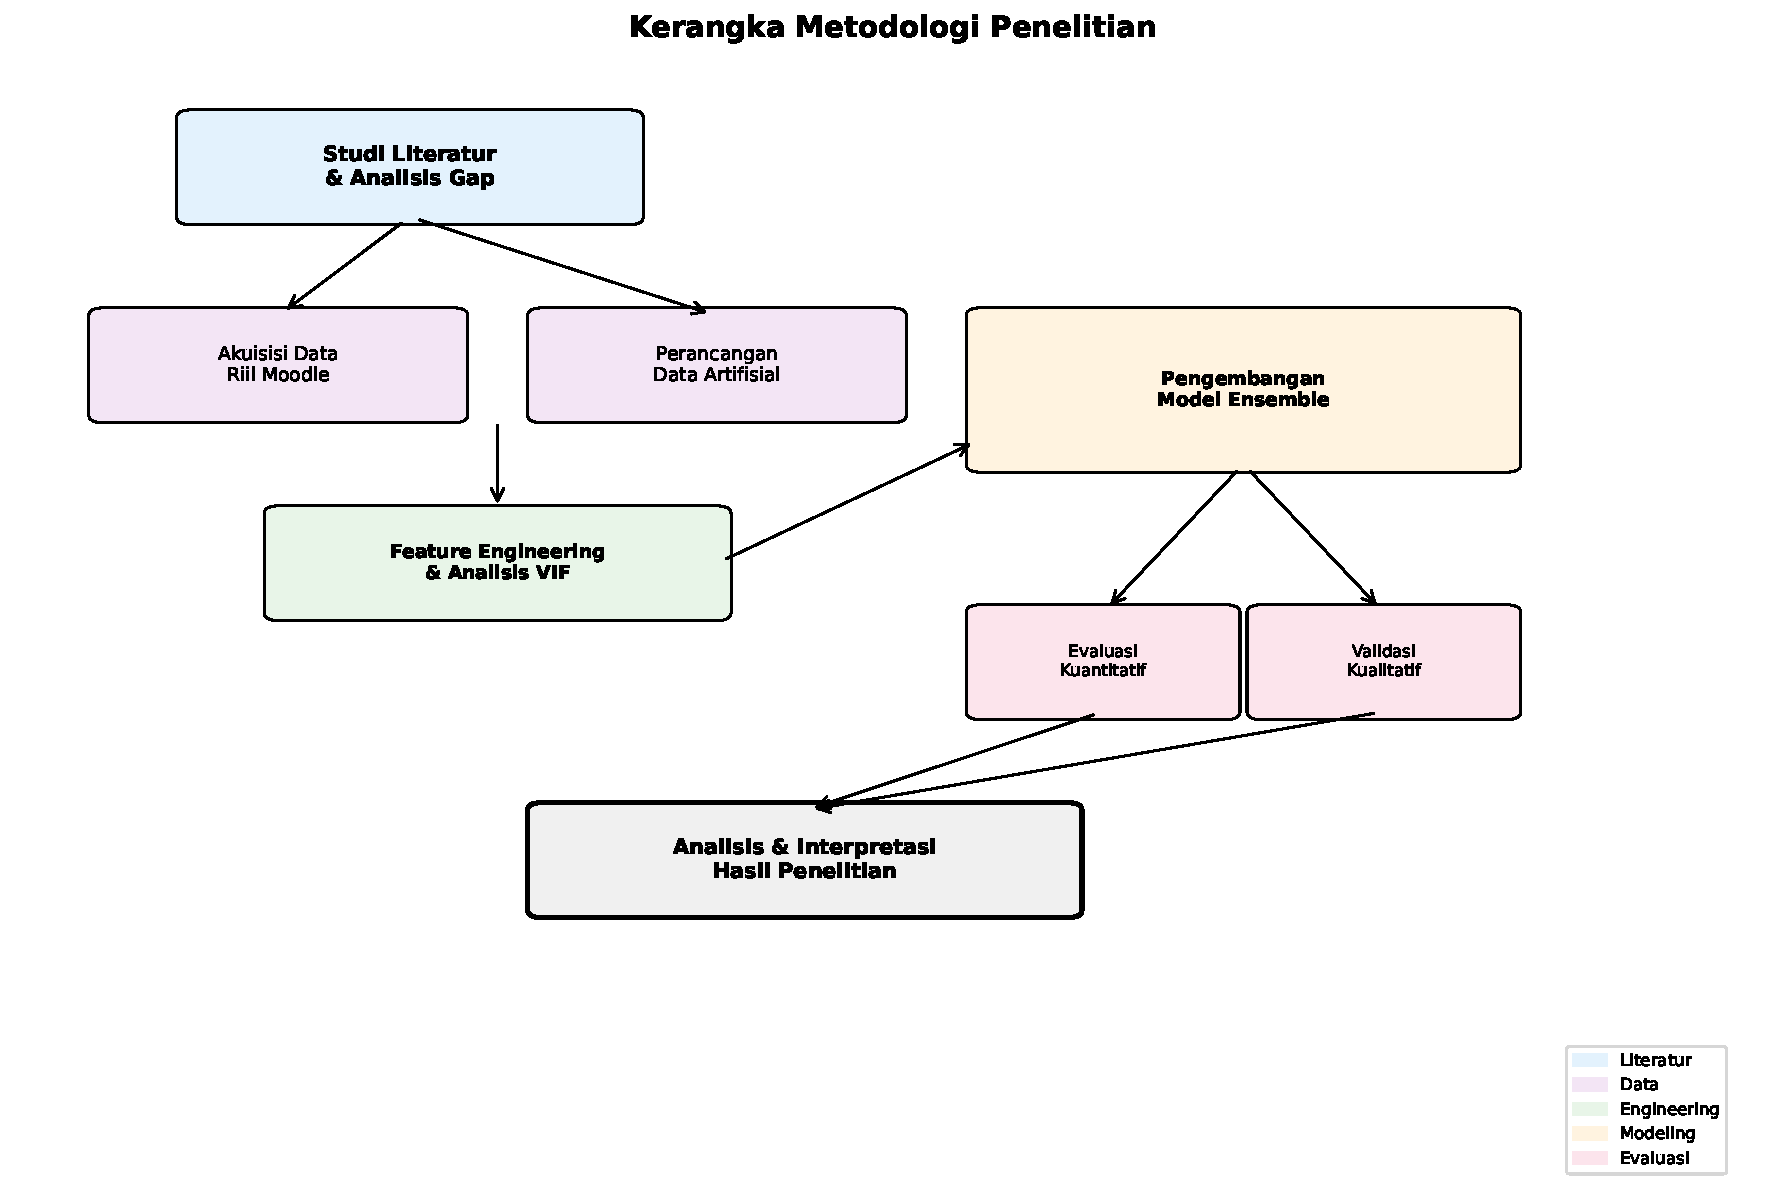
\includegraphics[width=0.95\textwidth]{newfigures/research_methodology_stages.pdf}
    \caption{Kerangka Metodologi Penelitian Deteksi Kecurangan}
    \label{fig:research_stages}
\end{figure}

Gambar \ref{fig:research_stages} menunjukkan kerangka metodologi penelitian yang terdiri dari enam fase utama yang saling berkaitan. Setiap fase dirancang secara spesifik untuk menjawab pertanyaan penelitian yang telah dirumuskan pada Bab 1. Fase 1 mengidentifikasi pola-pola kecurangan akademik melalui studi literatur. Fase 2 dan 3 mempersiapkan data pelatihan dengan \textit{ground truth} yang terkontrol. Fase 4 mentransformasi data mentah menjadi fitur-fitur bermakna. Fase 5 mengembangkan model deteksi menggunakan pendekatan \textit{ensemble}. Fase 6 mengevaluasi efektivitas model pada skala operasional.

\begin{figure}[htbp]
    \centering
    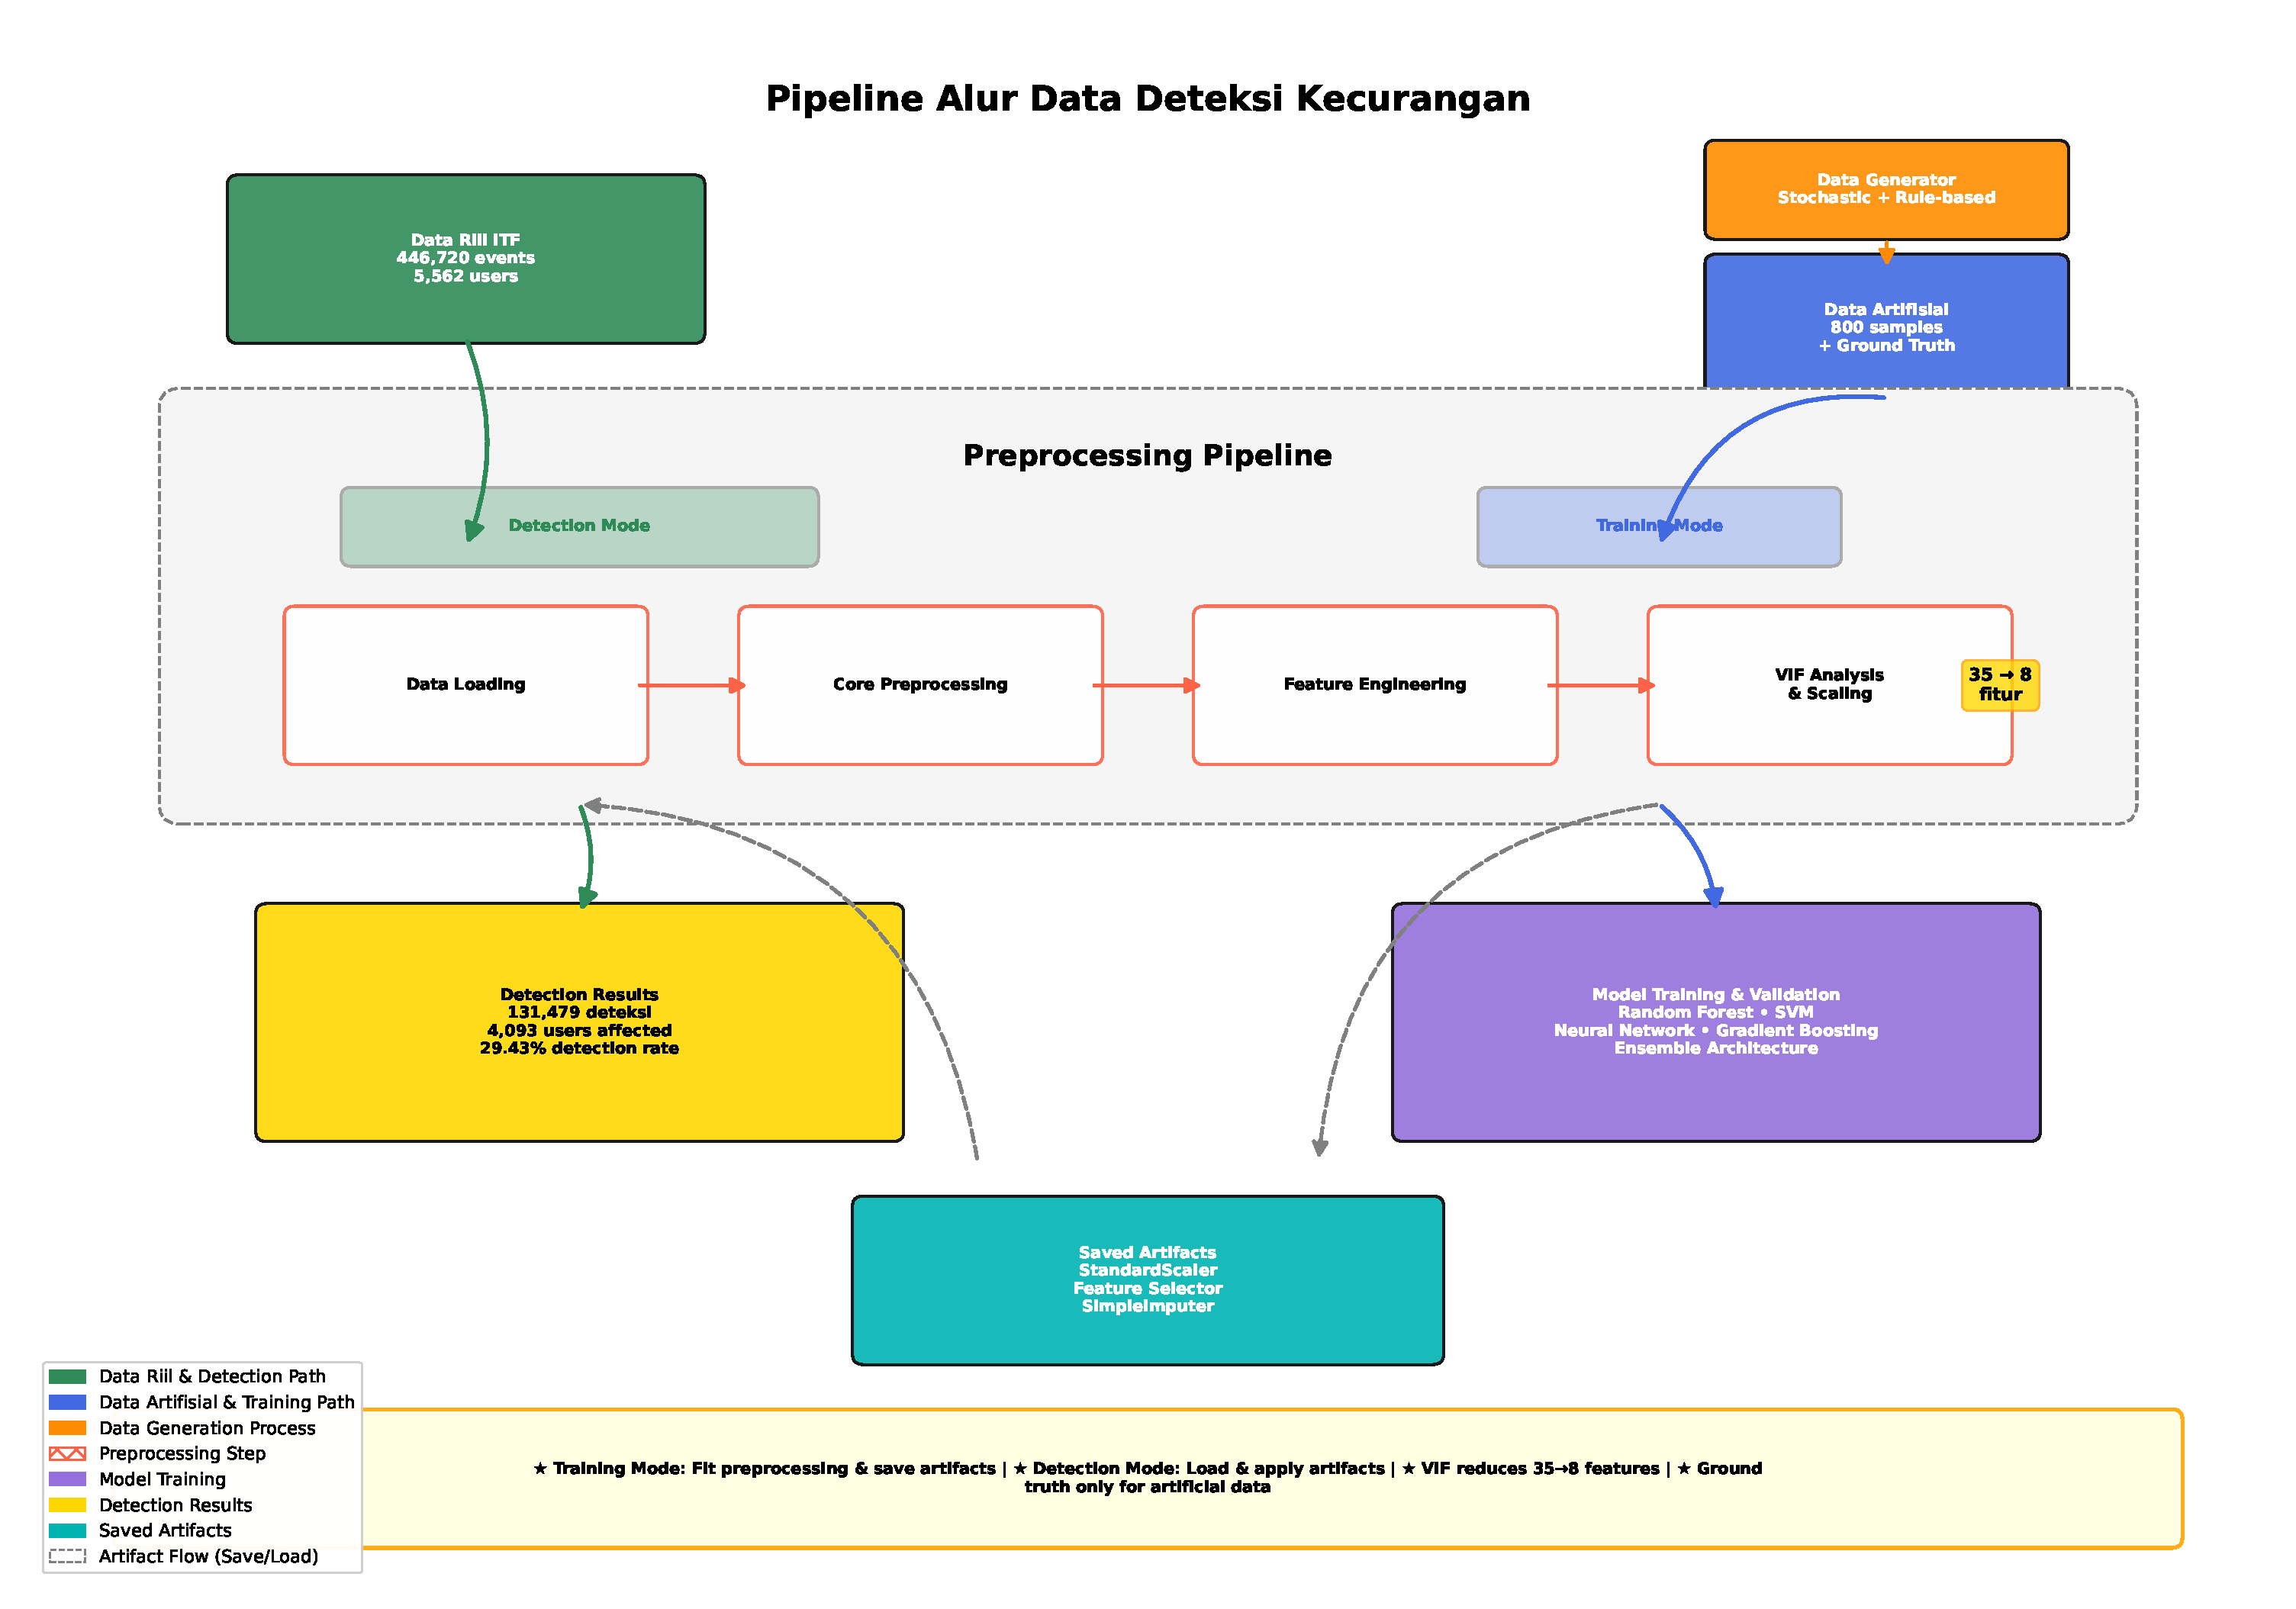
\includegraphics[width=0.98\textwidth]{newfigures/technical_pipeline_flow_final.pdf}
    \caption{Arsitektur Pipeline Teknis: Alur Pemrosesan Data dari Log Mentah hingga Deteksi Kecurangan dengan Dual-Mode Processing}
    \label{fig:technical_pipeline}
\end{figure}

Gambar \ref{fig:technical_pipeline} menerjemahkan kerangka metodologi konseptual menjadi implementasi teknis yang detail. \textit{Pipeline} dimulai dari dua sumber data yang berbeda karakteristiknya: \textbf{Data Riil ITF} yang berisi 446.720 \textit{events} dari aktivitas nyata mahasiswa Fasilkom UI, dan \textbf{Data Artifisial} dengan 800 sampel terkontrol yang dilengkapi \textit{ground truth} untuk pelatihan model. 

Perbedaan krusial terletak pada strategi pemrosesan: data artifisial diproses dalam \textit{Training Mode} untuk membangun dan menyimpan \textit{artifacts} pembelajaran (\textit{scaler}, \textit{feature selector}, \textit{imputer}), sementara data riil menggunakan \textit{Detection Mode} yang memanfaatkan \textit{artifacts} tersebut untuk konsistensi transformasi. \textit{Pipeline} berhasil mereduksi kompleksitas dari 35 fitur awal menjadi 8 fitur stabil melalui analisis \textit{Variance Inflation Factor} (VIF), menghasilkan model \textit{ensemble} yang mendeteksi 131.479 percobaan ujian mencurigakan (29,43\% dari total).

Kombinasi kedua diagram memberikan pemahaman menyeluruh: Gambar \ref{fig:research_stages} menyediakan peta konseptual untuk memandu pembaca melalui logika penelitian, sedangkan Gambar \ref{fig:technical_pipeline} memberikan \textit{blueprint} teknis untuk reproduksi penelitian. Integrasi pendekatan \textit{top-down} (konseptual) dan \textit{bottom-up} (teknis) ini memastikan transparansi metodologi yang dapat dipertanggungjawabkan secara ilmiah.

%-----------------------------------------------------------------------------%
%-----------------------------------------------------------------------------%
\section{Desain Penelitian dan Hipotesis}
\label{sec:desainPenelitian}
%-----------------------------------------------------------------------------%
Penelitian ini mengadopsi pendekatan eksperimental dengan kombinasi data artifisial dan riil untuk mengembangkan sistem deteksi kecurangan yang \textit{robust} (kokoh) dan dapat diimplementasikan dalam skala institusional. Desain penelitian dirancang secara sistematis untuk menjawab pertanyaan penelitian utama: bagaimana mengembangkan sistem deteksi kecurangan otomatis yang akurat untuk platform Moodle menggunakan pendekatan \textit{machine learning}?

\subsection{Alur Tahapan Penelitian}
\label{subsec:alurTahapanPenelitian}
Penelitian dilakukan melalui enam tahapan sistematis yang saling terkait:

\begin{enumerate}
    \item \textbf{Fase 1 - Analisis Kebutuhan dan Studi Literatur:} Mengidentifikasi pola-pola kecurangan akademik dalam pembelajaran daring melalui \textit{review} sistematis literatur. Fase ini menghasilkan pemahaman mendalam tentang karakteristik perilaku curang dan metode deteksi yang telah ada.
    
    \item \textbf{Fase 2 - Akuisisi Data Log Moodle:} Mengumpulkan data log aktivitas dari platform Moodle Fasilkom UI dengan total 446.720 \textit{events}. Data melalui proses anonimisasi untuk menjaga privasi pengguna.
    
    \item \textbf{Fase 3 - Perancangan Data Artifisial:} Mengembangkan generator data artifisial yang mensimulasikan 800 skenario ujian dengan parameter kecurangan terkontrol. Setiap skenario dilengkapi \textit{ground truth} untuk validasi model.
    
    \item \textbf{Fase 4 - Pengembangan \textit{Pipeline Preprocessing}:} Mengimplementasikan sistem ekstraksi dan transformasi fitur yang menghasilkan 35 fitur awal, kemudian direduksi menjadi 8 fitur stabil melalui analisis VIF.
    
    \item \textbf{Fase 5 - Pelatihan Model \textit{Ensemble}:} Melatih kombinasi algoritma \textit{Random Forest}, SVM, \textit{Neural Network}, dan \textit{Gradient Boosting} dengan optimasi \textit{hyperparameter} sistematis.
    
    \item \textbf{Fase 6 - Evaluasi Multi-Aspek:} Menguji model pada data artifisial (evaluasi kuantitatif) dan mengaplikasikan pada data riil (evaluasi kualitatif) untuk memvalidasi efektivitas deteksi.
\end{enumerate}

Setiap fase dirancang dengan \textit{output} yang jelas dan terukur, memungkinkan evaluasi progres penelitian secara objektif. Pendekatan iteratif diterapkan di mana hasil evaluasi dapat memicu perbaikan pada fase-fase sebelumnya.

\subsection{Hipotesis Penelitian}
\label{subsec:hipotesisPenelitian}
Berdasarkan studi literatur dan analisis awal, penelitian ini menguji empat hipotesis utama:

\textbf{H1: Deteksi Pola Kolaborasi}\\
Kolaborasi kecurangan akan menghasilkan pola similaritas yang dapat dideteksi dalam tiga dimensi: navigasi (urutan pengerjaan soal), \textit{timing} (pola waktu), dan jawaban (kesamaan respons). Hipotesis ini memprediksi tingkat akurasi deteksi $>90\%$ untuk kasus dengan koordinasi tinggi.

\textbf{H2: Superioritas Model Gabungan}\\
Model \textit{ensemble} (model gabungan) yang mengintegrasikan beberapa algoritma akan memberikan performa superior (peningkatan \textit{F1-score} minimal 5\%) dibandingkan model tunggal dalam mendeteksi berbagai strategi kecurangan yang heterogen.

\textbf{H3: \textit{Threshold} Ukuran Dataset}\\
Dataset dengan minimal 500-1000 sampel diperlukan untuk mencapai performa deteksi yang optimal (akurasi $>95\%$). Peningkatan ukuran dataset akan menghasilkan peningkatan performa yang signifikan hingga mencapai titik saturasi.

\textbf{H4: Generalisasi Model}\\
Model yang dilatih pada data artifisial dengan parameter terkontrol dapat menggeneralisasi dengan baik pada data riil skala besar, dengan tingkat deteksi yang konsisten dengan prevalensi kecurangan dalam literatur (20-40\%).

Keempat hipotesis ini akan diuji secara empiris melalui eksperimen yang dirancang dalam metodologi penelitian, dengan hasil pengujian disajikan pada Bab 4.

%-----------------------------------------------------------------------------%
%-----------------------------------------------------------------------------%
\section{Strategi Akuisisi dan Persiapan Data}
\label{sec:strategiAkuisisiData}
%-----------------------------------------------------------------------------%
Penelitian ini mengimplementasikan strategi \textit{dual-data} yang menggabungkan kekuatan data riil (validitas eksternal) dan data artifisial (kontrol internal) untuk mengoptimalkan pengembangan model deteksi kecurangan. Strategi ini memungkinkan pelatihan model dengan \textit{ground truth} yang terkontrol sambil mempertahankan kemampuan generalisasi pada kondisi operasional nyata.

%-----------------------------------------------------------------------------%
\section{Arsitektur Pipeline Preprocessing: Dari Log Mentah ke Fitur Terstruktur}
\label{sec:pipelinePreprocessing}
%-----------------------------------------------------------------------------%
\textit{Pipeline preprocessing} data merupakan komponen krusial yang mentransformasi log mentah Moodle menjadi representasi fitur yang siap untuk \textit{machine learning}. Sesuai dengan Fase 4 pada Gambar \ref{fig:research_stages}, \textit{pipeline} ini memproses kedua jenis data (riil dan artifisial) melalui empat modul terintegrasi dengan strategi \textit{dual-mode} yang memastikan konsistensi transformasi.

\subsection{Komponen dan Alur Kerja Pipeline}
\label{sec:komponenPipeline}

\textit{Pipeline preprocessing} dirancang dengan arsitektur modular yang terdiri dari empat komponen utama:

\textbf{Modul I - \textit{Data Loading} dan Validasi:} \\
Modul pertama bertanggung jawab memuat data dari berbagai tabel Moodle dengan validasi komprehensif. Tabel-tabel utama yang diproses meliputi mdl\_quiz\_attempts (percobaan ujian), mdl\_question\_attempt\_steps (langkah pengerjaan), dan mdl\_question\_attempt\_step\_data (detail jawaban). Validasi mencakup pemeriksaan tipe data, konsistensi referensial antar tabel, dan penanganan nilai yang hilang atau \textit{corrupt}. \textit{Output} modul ini adalah dataset terintegrasi yang siap untuk \textit{preprocessing} lanjutan.

\textbf{Modul II - \textit{Core Preprocessing} dan Normalisasi:} \\
Modul kedua melakukan pembersihan dan normalisasi fundamental. Proses utama meliputi: (1) unifikasi \textit{timestamp} ke format POSIX untuk konsistensi temporal, (2) penggabungan tabel-tabel terkait melalui \textit{foreign key} untuk membentuk \textit{event log} komprehensif, (3) \textit{filtering} data berdasarkan kriteria penelitian seperti status \textit{quiz completion}, dan (4) penghapusan duplikasi dan anomali data. Modul ini menghasilkan \textit{clean dataset} dengan struktur yang konsisten.

\textbf{Modul III - \textit{Feature Engineering} Multi-Dimensi:} \\
Modul ketiga mengekstraksi fitur-fitur \textit{behavioral} dari \textit{event log} yang telah dibersihkan. Ekstraksi fitur dilakukan dalam empat kategori:
\begin{itemize}
    \item \textbf{\textit{Intra-Attempt Features}:} Mengukur karakteristik dalam satu percobaan ujian seperti \textit{total duration}, \textit{number of actions}, dan \textit{step duration statistics}
    \item \textbf{\textit{Sequential Features}:} Menangkap pola urutan seperti \textit{navigation patterns}, \textit{revisit counts}, \textit{linearity measures}, dan entropi navigasi
    \item \textbf{\textit{Similarity Features}:} Menghitung kemiripan antar pengguna menggunakan \textit{Levenshtein distance} untuk navigasi dan korelasi statistik untuk \textit{timing patterns}
    \item \textbf{\textit{Comparative Features}:} Menormalkan perilaku individual terhadap populasi menggunakan transformasi \textit{z-score}
\end{itemize}

\textbf{Modul IV - \textit{Feature Selection} dan \textit{Optimization}:} \\
Modul terakhir melakukan optimasi fitur melalui beberapa tahap:
\begin{itemize}
    \item \textbf{\textit{Missing Value Imputation}:} Menggunakan \textit{SimpleImputer} dengan strategi \textit{mean} untuk fitur numerik
    \item \textbf{\textit{Multicollinearity Analysis}:} Menghitung \textit{Variance Inflation Factor} (VIF) dan mengeliminasi fitur dengan VIF $>10$
    \item \textbf{\textit{Variance Filtering}:} Menghilangkan fitur dengan \textit{variance} $<0,01$ yang tidak informatif
    \item \textbf{\textit{Standardization}:} Menerapkan \textit{StandardScaler} untuk normalisasi distribusi fitur
\end{itemize}

\subsection{Strategi \textit{Dual-Mode Processing}}
\label{sec:dualModeStrategy}

Inovasi kunci dalam \textit{pipeline} adalah implementasi \textit{dual-mode processing} yang membedakan pemrosesan data \textit{training} dan \textit{detection}:

\textbf{\textit{Training Mode} untuk Data Artifisial:} \\
Dalam \textit{mode training}, \textit{pipeline} melakukan \textit{fitting} terhadap data artifisial dan menyimpan semua \textit{transformation artifacts} ke direktori preprocessing/\textit{artifacts}/. \textit{Artifacts} yang disimpan meliputi: (1) \textit{fitted imputer} untuk menangani \textit{missing value}, (2) \textit{fitted scaler} dengan parameter \textit{mean} dan \textit{standard deviation}, (3) \textit{feature selector} dengan daftar fitur terpilih, dan (4) \textit{metadata} transformasi untuk \textit{reproducibility}. Mode ini memungkinkan eksplorasi parameter \textit{preprocessing} optimal melalui eksperimen terkontrol.

\textbf{\textit{Detection Mode} untuk Data Riil:} \\
Dalam \textit{mode detection}, \textit{pipeline} memuat \textit{artifacts} yang telah disimpan dan menerapkannya pada data riil tanpa melakukan \textit{fitting} ulang. Pendekatan ini memastikan: (1) konsistensi transformasi antara \textit{training} dan \textit{detection}, (2) pencegahan \textit{data leakage} dari \textit{test set}, (3) efisiensi komputasi dengan menghindari \textit{re-fitting}, dan (4) \textit{reproducibility} hasil deteksi. \textit{Pipeline} secara otomatis mendeteksi keberadaan \textit{artifacts} dan beralih ke mode yang sesuai.

Strategi \textit{dual-mode} ini merupakan \textit{best practice} dalam \textit{machine learning} yang memastikan validitas metodologis sambil mempertahankan efisiensi operasional. Transparansi penuh dalam proses transformasi memungkinkan audit dan verifikasi ilmiah terhadap setiap tahap \textit{preprocessing}.

\textbf{Data Riil Moodle:} \\
Data log \textit{Moodle} diperoleh langsung dari sistem yang dikelola oleh tim ITF Fasilkom UI dan telah melalui proses anonimisasi untuk menjaga privasi pengguna. Data ini digunakan untuk validasi model dalam konteks operasional nyata.

\textbf{Data Artifisial:} \\
Data artifisial dirancang khusus untuk pelatihan model dengan \textit{ground truth} yang terdokumentasi. Pendekatan ini memungkinkan eksplorasi berbagai skenario kecurangan dan kontrol parameter yang tidak mungkin dilakukan pada data riil.

\subsection{Data Log Moodle Riil: Deskripsi (periode, jumlah event/user, fitur utama), Proses Akuisisi, Kebijakan Anonimisasi \& Etika.}
\label{sec:logRiil}
Subbab ini menjelaskan mengenai data log yang diambil langsung dari sistem \textit{Moodle}, yang dikelola oleh tim ITF Fasilkom UI dan disimpan pada Lumbung Storage Cloud (mirip dengan platform penyimpanan seperti Google Drive). Data yang digunakan telah melalui proses anonimisasi, di mana identitas asli pengguna (username atau nama lengkap) tidak disertakan, melainkan hanya diwakili oleh \textit{user\_id}.

%-----------------------------------------------------------------------------%
\subsubsection{Deskripsi Data}
\label{sec:deskripsiData}
Data log \textit{Moodle} terdiri dari beberapa tabel utama yang masing-masing menyimpan informasi berbeda terkait aktivitas pengguna dan kuis. Berikut adalah rincian kolom-kolom yang terdapat dalam tiap tabel:

\textbf{mdl\_question\_usages} \\
Kolom: \textit{question\_usage\_id}, \textit{context\_id} \\
Menyimpan informasi terkait konteks penggunaan pertanyaan dalam kuis.

\textbf{mdl\_quiz\_grades} \\
Kolom: \textit{quiz\_grades\_id}, \textit{quiz\_id}, \textit{user\_id}, \textit{final\_grade} \\
Berisi nilai akhir dari masing-masing kuis yang diambil oleh pengguna.

\textbf{mdl\_question\_attempt\_steps} \\
Kolom: \textit{question\_step\_id}, \textit{question\_attempt\_id}, \textit{sequencenumber}, \textit{state}, \textit{timecreated} \\
Mencatat tiap langkah (\textit{step}) dalam upaya pengerjaan soal, termasuk status dan waktu pembuatan.

\textbf{mdl\_quiz\_attempts} \\
Kolom: \textit{attempt\_id}, \textit{quiz\_id}, \textit{user\_id}, \textit{question\_usage\_id}, \textit{timestart}, \textit{timefinish}, \textit{state}, \textit{sumgrades} \\
Menggambarkan detail setiap upaya pengerjaan kuis, termasuk waktu mulai, waktu selesai, status, dan jumlah nilai yang diperoleh. \\
Catatan: Terdapat anomali pada \textit{timefinish} (misalnya \textit{timestamp} 1970-01-01) yang kemungkinan menunjukkan upaya kuis yang belum selesai atau nilai \textit{default} dari \textit{Unix epoch}.

\textbf{mdl\_question\_answers} \\
Kolom: \textit{question\_answers\_id}, \textit{questionid}, \textit{answer\_text}, \textit{fraction} \\
Menyimpan data mengenai jawaban yang diberikan pada tiap pertanyaan, termasuk teks jawaban dan bobot nilai yang terkait.

\textbf{mdl\_question\_attempt\_step\_data} \\
Kolom: \textit{step\_data\_id}, \textit{question\_step\_id}, \textit{name}, \textit{value} \\
Menyimpan data tambahan terkait langkah pengerjaan soal, yang dapat berupa nilai-nilai pendukung dari proses evaluasi.

\textbf{mdl\_quiz} \\
Kolom: \textit{quiz\_id}, \textit{course}, \textit{quiz\_name}, \textit{timeopen}, \textit{timeclose}, \textit{timelimit} \\
Berisi informasi dasar mengenai kuis, termasuk mata kuliah, nama kuis, serta waktu buka dan tutup kuis.

\textbf{mdl\_sessions} \\
Kolom: \textit{session\_id}, \textit{user\_id}, \textit{timecreated}, \textit{lastip}, \textit{sessdata} \\
Mencatat aktivitas sesi pengguna, mulai dari waktu pembuatan sesi hingga informasi terkait IP dan data sesi lainnya.

%-----------------------------------------------------------------------------%
\subsubsection{Rentang Waktu dan Skala Dataset}
\label{sec:rentangWaktuSkalaDataset}
Data log \textit{Moodle} mencakup periode hampir 10 tahun, dengan rentang data keseluruhan dari tanggal 31 Juli 2015 hingga 22 Februari 2025. Secara spesifik:

\textbf{mdl\_question\_attempt\_steps:} \\
Rentang waktu: 29 Agustus 2015--22 Februari 2025 \\
Durasi: sekitar 3.565 hari

\textbf{mdl\_quiz\_attempts:} \\
Rentang waktu untuk \textit{timestart}: 31 Juli 2015--22 Februari 2025 \\
Rentang waktu untuk \textit{timefinish}: (dengan catatan anomali \textit{timestamp} 1970 sebagai \textit{default}) hingga 22 Februari 2025 \\
Durasi: sekitar 3.594 hari (mengabaikan nilai \textit{default} 1970)

\textbf{mdl\_sessions:} \\
Rentang waktu: 17 Maret 2020--22 Februari 2025 \\
Durasi: sekitar 1.803 hari

Skala data secara keseluruhan meliputi:
\begin{itemize}
    \item Total kuis yang diambil: 446.720 upaya
    \item Jumlah pengguna unik: 5.562
    \item Jumlah kuis unik: 6.304
    \item Jumlah langkah pertanyaan: 22.192.809
\end{itemize}

%-----------------------------------------------------------------------------%
\subsubsection{Cakupan Mata Kuliah dan Pola Penggunaan}
\label{sec:cakupanMataKuliahPolaPenggunaan}
Data ini mencakup aktivitas di lebih dari 140 Mata Kuliah unik, dengan variasi ukuran kelas:

\textbf{Ukuran Mata Kuliah:}
\begin{itemize}
    \item Mata Kuliah besar (300+ mahasiswa): sekitar 10 Mata Kuliah
    \item Mata Kuliah menengah (100-300 mahasiswa): sekitar 30 Mata Kuliah
    \item Mata Kuliah kecil ($<100$ mahasiswa): sekitar 100 Mata Kuliah
    \item Mata Kuliah sangat kecil ($<10$ mahasiswa): sekitar 15 Mata Kuliah
\end{itemize}

\textbf{Contoh Mata Kuliah dengan aktivitas tinggi:}
\begin{itemize}
    \item Mata Kuliah 3836: 453 peserta, 5.544 upaya (rata-rata 12,24 upaya per pengguna)
    \item Mata Kuliah 3634: 442 peserta, 5.902 upaya (rata-rata 13,35 upaya per pengguna)
    \item Mata Kuliah 3723: 390 peserta, 3.829 upaya (rata-rata 9,56 upaya per pengguna)
    \item Mata Kuliah 3640: 386 peserta, 4.463 upaya (rata-rata 11,56 upaya per pengguna)
    \item Mata Kuliah 3636: 382 peserta, 761 upaya (rata-rata 1,99 upaya per pengguna)
\end{itemize}

Pola penggunaan kuis menunjukkan perbedaan yang signifikan antar Mata Kuliah. Beberapa Mata Kuliah hanya mencatat satu upaya per pengguna, sedangkan Mata Kuliah lain mencatat rata-rata 10 upaya atau lebih, yang mengindikasikan adanya kuis latihan atau kebijakan pengulangan untuk meningkatkan pemahaman materi.

%-----------------------------------------------------------------------------%
\subsubsection{Proses Akuisisi dan Kebijakan Anonimisasi}
\label{sec:prosesAkuisisiKebijakanAnonimisasi}
Data log \textit{Moodle} diakuisisi secara langsung dari sistem \textit{Moodle} oleh tim ITF Fasilkom UI dan kemudian disimpan di Lumbung Storage Cloud. Proses akuisisi melibatkan:

\textbf{Pengambilan Data:} \\
Data diekstraksi dari server \textit{Moodle} dengan menggunakan prosedur logging yang telah ditetapkan, memastikan setiap aktivitas terekam secara lengkap.

\textbf{Pengiriman dan Penyimpanan:} \\
Data dikirim dan disimpan secara terpusat di Lumbung Storage Cloud yang merupakan \textit{repository} internal Fasilkom UI, menjamin keamanan dan integritas data.

\textbf{Anonimisasi:} \\
Untuk melindungi privasi pengguna, data telah diproses sehingga informasi identitas pribadi (username, nama lengkap, dan data sensitif lainnya) dihilangkan. Hanya \textit{user\_id} yang tetap dipertahankan untuk keperluan analisis. Hal ini sesuai dengan standar etika penelitian dan kebijakan perlindungan data yang berlaku.

\textbf{Pertimbangan Etika:} \\
Penggunaan data riil ini telah mempertimbangkan aspek etika dan regulasi perlindungan data. Kebijakan anonimisasi yang diterapkan memastikan bahwa data tidak dapat dikaitkan langsung dengan individu tertentu, sehingga menjaga kerahasiaan dan privasi pengguna.

%-----------------------------------------------------------------------------%
\subsection{Strategi Data Artifisial}
\label{sec:dataArtifisial}
%-----------------------------------------------------------------------------%
Data artifisial dalam penelitian ini dirancang untuk mengatasi keterbatasan \textit{ground truth} pada data riil. Strategi ini memungkinkan kontrol penuh terhadap parameter kecurangan dan validasi objektif terhadap performa model, dengan alasan-alasan sebagai berikut:

\begin{enumerate}
    \item \textbf{Kontrol Variabel dan Simulasi Skenario Ekstrem:} \\
    Data artifisial memungkinkan penciptaan skenario perilaku pengguna yang ekstrem atau tidak biasa, yang mungkin jarang terjadi pada data log riil. Dengan demikian, model dapat dilatih untuk mengenali pola-pola \textit{non-compliance} secara lebih spesifik dan mendalam.
    
    \item \textbf{Pengembangan Model yang Terarah:} \\
    Dalam penelitian ini, pengembangan model dilakukan sepenuhnya dengan menggunakan data artifisial. Pendekatan ini memberikan fleksibilitas dalam mengatur parameter dan iterasi pelatihan, serta mengurangi risiko \textit{overfitting} pada data riil yang belum terlabel dengan jelas.
    
    \item \textbf{Evaluasi Model dengan Data Riil:} \\
    Setelah model dioptimasi dengan data artifisial, evaluasi akhir akan dilakukan dengan menerapkan model pada data log asli. Langkah ini bertujuan untuk mengukur sejauh mana model dapat mendeteksi kasus kecurangan yang benar-benar terjadi di lingkungan sistem \textit{Moodle}, sehingga memberikan validasi nyata terhadap efektivitas pendekatan yang digunakan.
    
    \item \textbf{Pendekatan Metodologis dalam Pembuatan Data Artifisial:} \\
    Data artifisial dihasilkan melalui kombinasi simulasi berbasis aturan dan proses stokastik, yang disesuaikan dengan pola penggunaan yang ditemukan dalam data log riil. Pendekatan ini memastikan bahwa data artifisial tidak hanya mereplikasi kondisi normal, tetapi juga memasukkan skenario \textit{non-compliance} yang relevan untuk pengembangan model.
\end{enumerate}

Dengan demikian, penggunaan data artifisial dalam penelitian ini memberikan keuntungan dalam hal kontrol variabilitas dan eksplorasi skenario ekstrem, serta mempercepat proses pengembangan model. Evaluasi akhir dengan data log riil akan menjadi tolok ukur untuk menilai kemampuan model dalam mendeteksi kecurangan yang terjadi secara nyata dalam sistem \textit{Moodle}.

%-----------------------------------------------------------------------------%
\section{Preprocessing Pipeline dan Feature Engineering}
\label{sec:preprocessingPipelineFeatureEngineering}
%-----------------------------------------------------------------------------%
Tahap \textit{feature engineering} dan analisis VIF merupakan komponen kritis dalam \textit{pipeline} penelitian ini. Proses ini mencakup transformasi data mentah menjadi representasi fitur yang bermakna, analisis multikolinearitas, dan seleksi fitur optimal untuk model \textit{machine learning}. 

\begin{figure}[htbp]
    \centering
    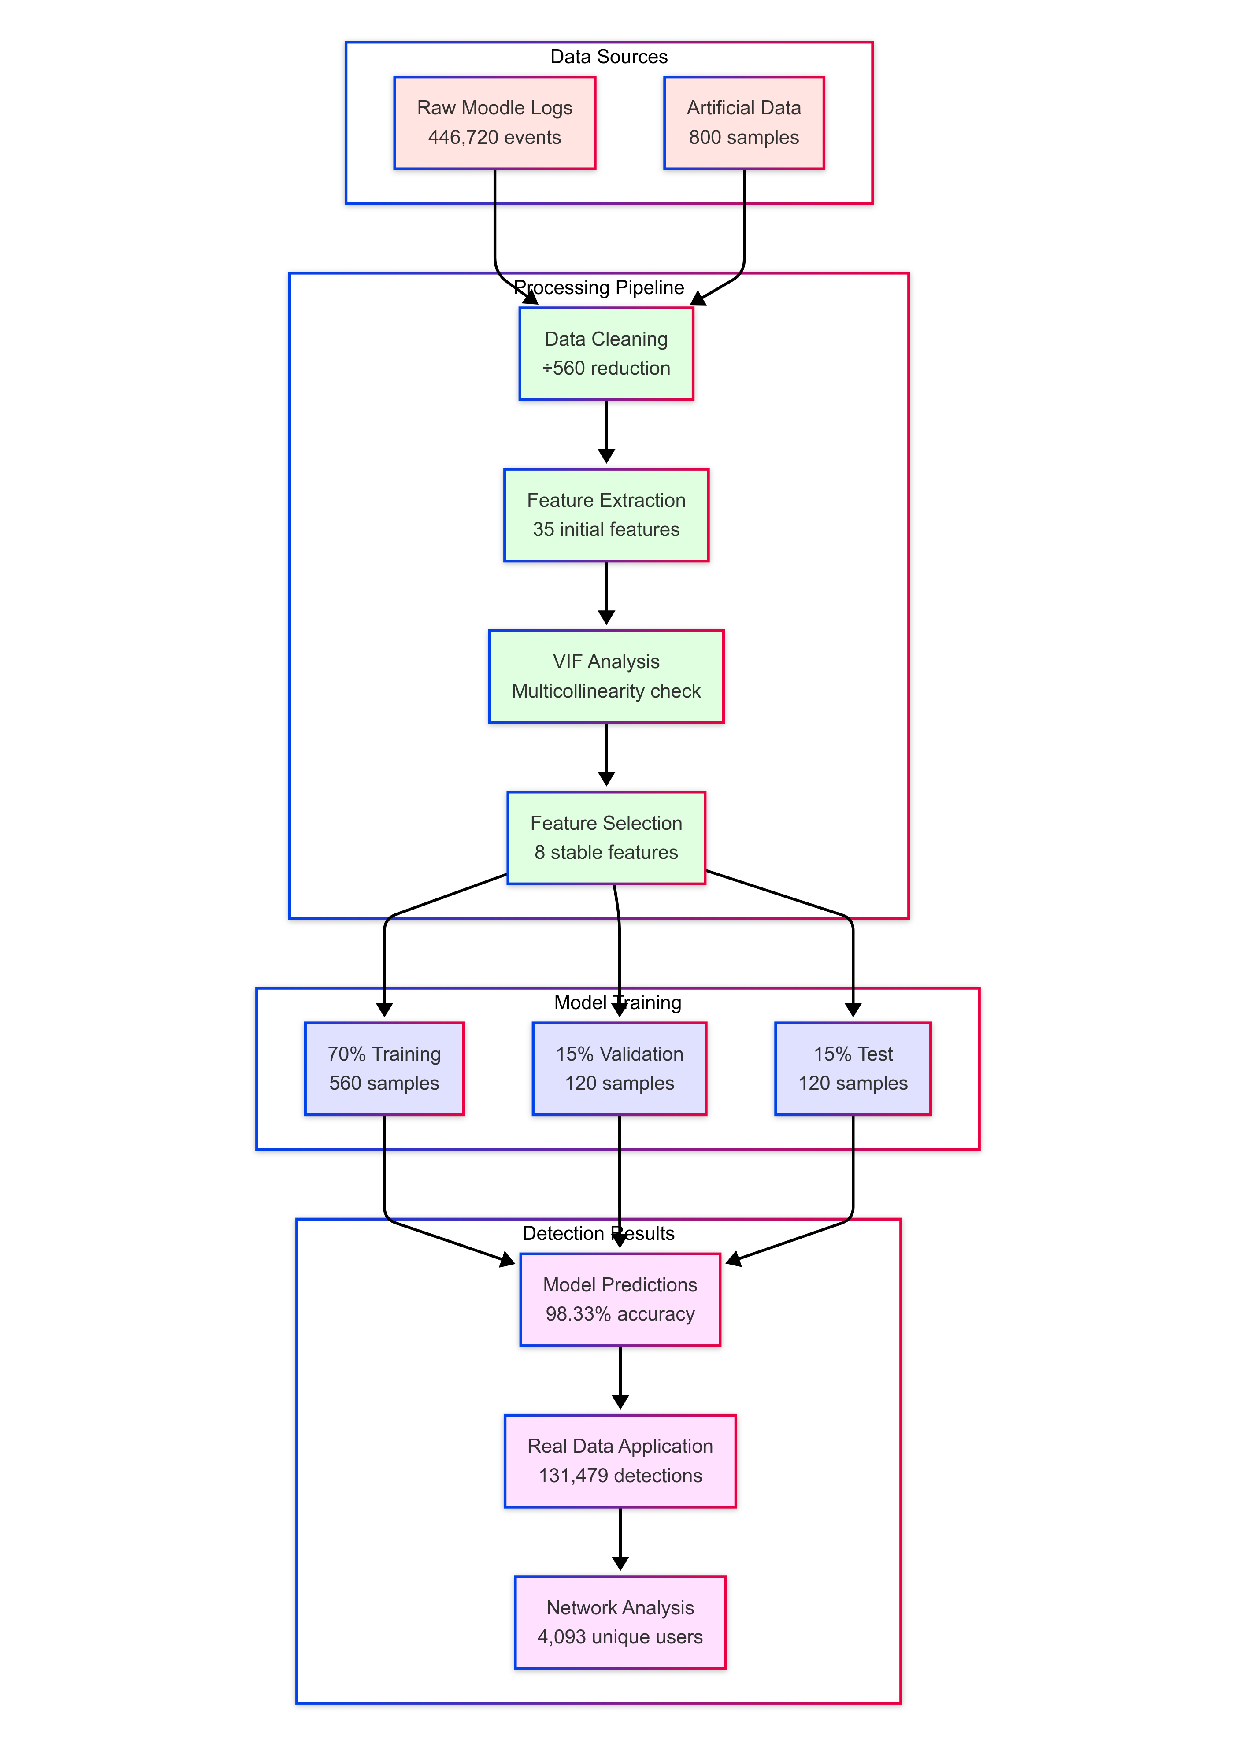
\includegraphics[width=0.95\textwidth]{figures/data_flow_diagram.pdf}
    \caption{Alur Data dalam \textit{Pipeline} Deteksi Kecurangan}
    \label{fig:data_flow}
\end{figure}

Gambar \ref{fig:data_flow} menunjukkan alur transformasi data dari \textit{raw logs} hingga \textit{detection output}. Reduksi dramatis dari 446.720 \textit{events} menjadi 800 \textit{training samples} (faktor 560x) dilakukan melalui agregasi per \textit{user-quiz attempt}. \textit{Feature extraction} menghasilkan 35 fitur awal yang kemudian direduksi menjadi 8 fitur stabil melalui \textit{VIF analysis}. Data dibagi dengan proporsi 70/15/15 untuk \textit{training}, \textit{validation}, dan \textit{test} untuk memastikan evaluasi yang adil dan mencegah \textit{overfitting}.

Proses pra-pemrosesan tidak hanya bertujuan untuk mengurangi gangguan dan inkonsistensi, tetapi juga untuk memastikan bahwa fitur-fitur yang dihasilkan mencerminkan karakteristik perilaku pengguna secara akurat. Langkah-langkah berikut diambil dengan dasar metodologis yang dapat dipertahankan secara ilmiah:

%-----------------------------------------------------------------------------%
\subsection{Pembersihan Data (Data Cleaning)}
\label{sec:pembersihanData}
%-----------------------------------------------------------------------------%
\textbf{Penanganan \textit{Missing Values}:} \\
Data log sering kali mengandung nilai yang hilang (\textit{missing values}) karena ketidakteraturan dalam pencatatan \textit{event} atau \textit{error} saat pengambilan data. Dalam \textit{pipeline}, nilai yang tidak terisi diimputasi dengan metode penggantian menggunakan nilai \textit{default} (misalnya, 0) atau perhitungan statistik (rata-rata/median) ketika relevan. Misalnya, dalam skrip \texttt{preprocess\_features.py}, setelah ekstraksi fitur, seluruh nilai NaN diisi dengan nol untuk memastikan tidak ada celah data yang dapat mengganggu analisis model.

\textbf{\textit{Filtering} Data yang Tidak Relevan:} \\
Dalam konteks deteksi kecurangan, tidak seluruh \textit{event log} memiliki nilai informasi yang sama. Oleh karena itu, dilakukan penyaringan untuk:
\begin{itemize}
    \item Mengabaikan \textit{event} dengan atribut tertentu (misalnya, \textit{field} \textit{contextlevel} yang bernilai '\textit{system}') karena \textit{event} ini tidak mewakili aktivitas pengguna pada kuis.
    \item Menghapus entri dengan \textit{user\_id} yang \textit{null}, mengingat identifikasi pengguna merupakan variabel kunci dalam analisis pola perilaku.
\end{itemize}

%-----------------------------------------------------------------------------%
\subsection{Transformasi dan Normalisasi Data}
\label{sec:transformasiNormalisasiData}
%-----------------------------------------------------------------------------%
\textbf{Unifikasi Format Waktu dan Normalisasi Zona Waktu:} \\
Data log mengandung \textit{timestamp} yang berasal dari sumber atau zona waktu yang berbeda. Untuk memastikan keseragaman, seluruh \textit{timestamp} dikonversi ke dalam format numerik, seperti \textit{Unix timestamp} (atau ISO 8601 jika diperlukan), melalui fungsi konversi di \texttt{preprocess\_features.py}. Proses ini juga melibatkan normalisasi zona waktu agar seluruh \textit{event log} dapat dibandingkan secara akurat dalam kerangka waktu yang sama.

\textbf{\textit{Parsing Nested Fields}:} \\
Banyak kolom dalam data log disimpan dalam bentuk \textit{string} yang merepresentasikan \textit{array} atau \textit{dictionary} (misalnya, \textit{sequence} navigasi atau \textit{transition times}). Menggunakan fungsi seperti \texttt{ast.literal\_eval}, skrip melakukan \textit{parsing} terhadap \textit{string} tersebut sehingga struktur data yang tersusun (\textit{list} atau \textit{dictionary}) dapat diekstraksi. Proses ini memungkinkan perhitungan fitur statistik seperti panjang \textit{sequence}, entropi, dan jumlah \textit{revisits}, yang esensial untuk mendeteksi pola aktivitas pengguna.

%-----------------------------------------------------------------------------%
\subsection{Ekstraksi Fitur dan Deteksi Outlier}
\label{sec:ekstraksiFiturDeteksiOutlier}
%-----------------------------------------------------------------------------%
Setelah data dibersihkan dan ditransformasikan, tahap selanjutnya adalah ekstraksi fitur, di mana fitur-fitur dasar dan lanjutan dihasilkan untuk mendukung proses pelatihan model deteksi kecurangan. Dalam \textit{pipeline}, ekstraksi fitur dilakukan melalui modul \texttt{feature\_eng.py} dan \texttt{fixed\_extraction.py}, dengan beberapa langkah sebagai berikut:

\textbf{Fitur Dasar:} \\
Fitur seperti jumlah percobaan kuis, rata-rata waktu pengerjaan, total waktu, serta statistik minimum dan maksimum dihitung dari data log kuis. Contoh implementasi terdapat pada fungsi \texttt{extract\_basic\_statistics()} di \texttt{feature\_eng.py}, yang juga menyertakan agregasi data per pasangan \textit{user}-kuis.

\textbf{Fitur \textit{Sequence}:} \\
Dari data navigasi dan jawaban, diekstraksi fitur-fitur seperti:
\begin{itemize}
    \item Panjang \textit{sequence} dan jumlah pertanyaan unik: Mengukur seberapa panjang dan bervariasinya aktivitas navigasi pengguna.
    \item \textit{Linearity}: Menghitung seberapa berurutan langkah-langkah yang diambil, menggunakan perhitungan rasio antara pertanyaan unik dan total langkah.
    \item \textit{Revisits}: Penghitungan jumlah \textit{revisits} atau langkah yang diulang, sebagai indikasi pola abnormal.
\end{itemize}
Fungsi \texttt{extract\_navigation\_features()} dalam \texttt{fixed\_extraction.py} mengilustrasikan bagaimana fitur-fitur tersebut dihitung dengan memanfaatkan evaluasi \textit{list} dari \textit{sequence}.

\textbf{Deteksi \textit{Outlier} pada Fitur Waktu:} \\
Pada ekstraksi fitur waktu, dilakukan perhitungan statistik seperti rata-rata, standar deviasi, nilai minimum dan maksimum dari durasi pengerjaan soal. Selain itu, skrip juga menghitung jumlah \textit{event} dengan durasi sangat pendek (misalnya, $< 5$ detik) dan sangat panjang (misalnya, $> 600$ detik).

Berikut adalah cuplikan kode dari fungsi \texttt{extract\_timing\_features()} yang digunakan untuk mendeteksi pola waktu yang abnormal, yang dapat dijadikan indikator \textit{outlier}:

\begin{verbatim}
def extract_timing_features(time_seq):
    """Ekstraksi fitur dari sequence waktu."""
    features = {}
    
    try:
        if isinstance(time_seq, str):
            time_seq = eval(time_seq)
        time_seq = np.array(time_seq, dtype=float)
        
        features['mean_time'] = float(np.mean(time_seq))
        features['std_time'] = float(np.std(time_seq))
        features['min_time'] = float(np.min(time_seq))
        features['max_time'] = float(np.max(time_seq))
        
        # Pola waktu mencurigakan sebagai indikator outlier
        features['quick_answers'] = int(sum(1 for t in time_seq if t < 5))
        features['very_long_answers'] = int(sum(1 for t in time_seq if t > 600))
    except Exception as e:
        print(f"Warning: Error processing timing features: {e}")
        features['mean_time'] = 0.0
        features['std_time'] = 0.0
        features['min_time'] = 0.0
        features['max_time'] = 0.0
        features['quick_answers'] = 0
        features['very_long_answers'] = 0
    
    return features
\end{verbatim}

Nilai \texttt{quick\_answers} dan \texttt{very\_long\_answers} ini memberikan gambaran tentang berapa kali pengguna menyelesaikan bagian tertentu dengan durasi yang sangat tidak wajar, yang kemudian dapat diintegrasikan sebagai fitur untuk mendeteksi perilaku kecurangan.

\textbf{Penghitungan \textit{Similarity Features}:} \\
Untuk mendeteksi kolaborasi kecurangan, \textit{pipeline} menghitung matriks kemiripan (\textit{similarity matrix}) berdasarkan pola navigasi, waktu, dan jawaban antar pengguna. Fungsi \texttt{calculate\_similarity\_matrices()} di \texttt{feature\_eng.py} menghitung kemiripan menggunakan metode seperti \textit{Levenshtein distance} untuk \textit{sequence} navigasi dan korelasi untuk \textit{sequence} waktu, kemudian hasilnya digunakan untuk menambahkan fitur agregat seperti rata-rata dan maksimum \textit{similarity} antar pengguna.



%-----------------------------------------------------------------------------%

%-----------------------------------------------------------------------------%
\subsection{\textit{Checklist} Pra-pemrosesan}
\label{sec:checklistPraPemrosesan}
%-----------------------------------------------------------------------------%
Untuk memastikan bahwa seluruh proses pra-pemrosesan dapat diulangi dan diverifikasi, disusunlah \textit{checklist} sebagai berikut:
\begin{itemize}
    \item Konversi seluruh \textit{timestamp} ke format standar (\textit{Unix timestamp} atau ISO 8601).
    \item Penghapusan \textit{event} dengan atribut \textit{contextlevel} bernilai '\textit{system}'.
    \item Penyaringan entri dengan \textit{user\_id} \textit{null}.
    \item \textit{Parsing} kolom yang berisi \textit{string} representasi \textit{array}/\textit{dict} untuk ekstraksi fitur.
    \item Normalisasi zona waktu untuk keseragaman data.
    \item Perhitungan statistik fitur dasar dan \textit{sequence} (termasuk deteksi pola \textit{outlier} pada waktu).
\end{itemize}

%-----------------------------------------------------------------------------%
\subsection{Justifikasi Ilmiah}
\label{sec:justifikasiIlmiah}
%-----------------------------------------------------------------------------%
Pendekatan pra-pemrosesan yang diterapkan dalam penelitian ini didasarkan pada prinsip-prinsip \textit{data cleaning} dan \textit{feature engineering} yang telah terbukti secara empiris meningkatkan kualitas \textit{dataset} dan kinerja model \textit{machine learning}.

\textbf{Pembersihan dan Transformasi:} \\
Dengan memastikan bahwa data dalam format yang konsisten dan bebas dari \textit{missing values}, variabilitas yang tidak relevan dapat diminimalkan, sehingga model tidak terdistorsi oleh gangguan data.

\textbf{Ekstraksi Fitur:} \\
Fitur-fitur yang diekstraksi, seperti \textit{linearity} dan \textit{revisits} pada \textit{sequence}, memberikan representasi numerik yang dapat menggambarkan perilaku pengguna secara mendalam.

\textbf{Deteksi \textit{Outlier}:} \\
Dengan mengidentifikasi \textit{event} dengan durasi yang sangat singkat atau sangat panjang, \textit{pipeline} mampu memberikan sinyal peringatan terhadap kemungkinan aktivitas yang tidak wajar, yang secara langsung berkontribusi pada identifikasi kecurangan.

\textbf{\textit{Reproducibility}:} \\
\textit{Checklist} dan struktur modular pada skrip memastikan bahwa seluruh proses dapat direplikasi dan diaudit, sehingga mendukung validitas dan \textit{reproducibility} dari penelitian.

Melalui serangkaian proses yang sistematis dan berbasis algoritma yang telah teruji, tahap pra-pemrosesan ini memberikan dasar yang kuat untuk langkah-langkah selanjutnya dalam \textit{pipeline}, yaitu ekstraksi fitur lanjutan, pelatihan model, dan akhirnya evaluasi deteksi kecurangan.

%-----------------------------------------------------------------------------%
\subsection{Perancangan dan Generasi Data Artifisial}
\label{sec:perancanganGenerasiDataArtifisial}
%-----------------------------------------------------------------------------%
Subbab ini menjelaskan secara mendalam mengenai rancangan, implementasi, dan validasi data log \textit{Moodle} artifisial yang digunakan untuk mengembangkan model deteksi \textit{non-compliance}. Pendekatan yang diterapkan dikenal dengan istilah \textit{Skenario Perilaku Sintetik}, yaitu simulasi aktivitas pengguna (baik perilaku normal maupun \textit{non-compliance}) melalui algoritma yang menggabungkan simulasi berbasis aturan dan proses stokastik. Data artifisial ini tidak hanya mereplikasi aktivitas log riil, tetapi juga memungkinkan eksplorasi skenario ekstrem yang jarang terekam pada data nyata, seperti koordinasi kelompok kecurangan dengan pola sinkronisasi tinggi.

%-----------------------------------------------------------------------------%
\subsection{Definisi Operasional Skenario Perilaku Sintetik}
\label{sec:definisiOperasionalSkenarioPerilakuSintetik}
%-----------------------------------------------------------------------------%
Skenario Perilaku Sintetik didefinisikan sebagai rangkaian aturan dan mekanisme yang dirancang untuk mereplikasi pola aktivitas pengguna pada sistem \textit{Moodle}, baik dalam kondisi normal maupun \textit{non-compliance} (kecurangan). Pendekatan ini mengintegrasikan simulasi berbasis aturan dengan proses stokastik, sehingga memungkinkan pembentukan data log artifisial yang tidak hanya mereplikasi aktivitas log riil, tetapi juga dapat mengeksplorasi skenario ekstrem yang jarang terekam dalam data nyata.

\textbf{Perilaku Normal:} \\
Pada skenario perilaku normal, aktivitas pengguna dirancang untuk mencerminkan dinamika berpikir yang alami, yang ditandai dengan:
\begin{itemize}
    \item Variasi Urutan Navigasi: Pengguna normal menunjukkan urutan akses pertanyaan yang bervariasi, dengan kemungkinan revisi jawaban yang berbeda-beda antar sesi. Hal ini menggambarkan proses evaluasi internal yang dinamis.
    \item Variasi Pola Jawaban: Pola jawaban mencerminkan respon acak yang wajar, dengan proporsi jawaban benar dan salah yang bervariasi secara alami.
    \item Waktu Pengerjaan yang Variatif: Interval waktu antar pertanyaan bervariasi, mencerminkan kecepatan berpikir dan penyesuaian terhadap tingkat kesulitan pertanyaan. Distribusi waktu pengerjaan ini umumnya menunjukkan standar deviasi yang wajar.
\end{itemize}

\textbf{Perilaku \textit{Non-Compliance} (Kecurangan):} \\
Pada skenario \textit{non-compliance}, pola aktivitas sengaja diatur untuk menciptakan indikasi kecurangan, dengan karakteristik sebagai berikut:
\begin{itemize}
    \item Kesamaan Navigasi: Urutan pertanyaan yang diakses oleh pengguna dalam kelompok kecurangan sangat mirip, termasuk adanya revisi yang identik antar anggota kelompok.
    \item Konsistensi Jawaban: Pola jawaban menunjukkan tingkat keseragaman yang tinggi. Misalnya, terdapat kecenderungan anggota kelompok secara bersama-sama memberikan jawaban salah pada pertanyaan-pertanyaan sulit.
    \item Sinkronisasi Waktu yang Tidak Wajar: Interval waktu antar pertanyaan hampir seragam antar pengguna. Dalam beberapa kasus, terdapat kelompok yang menyelesaikan kuis secara bersamaan dalam waktu kurang dari 15 detik, dengan standar deviasi yang rendah, mengindikasikan adanya pola sinkronisasi yang sulit terjadi secara alami.
    \item Mekanisme \textit{Leader-Follower}: Terdapat pola di mana satu anggota (\textit{leader}) menyelesaikan kuis terlebih dahulu, sedangkan anggota lainnya (\textit{follower}) mengikuti dengan \textit{delay} yang konsisten. Pola ini menciptakan korelasi tinggi dalam waktu pengerjaan antar anggota, yang menjadi indikator kuat adanya koordinasi.
\end{itemize}

Definisi operasional ini menjadi dasar untuk memformulasikan parameter simulasi. Parameter-parameter tersebut, seperti tingkat kemiripan navigasi, \textit{delay} waktu, dan distribusi jawaban, kemudian diintegrasikan dalam algoritma generasi data log artifisial. Setiap skenario diberikan label \textit{ground truth}, yang memungkinkan validasi dan evaluasi model deteksi kecurangan secara kuantitatif dan kualitatif.

%-----------------------------------------------------------------------------%
\subsection{Desain \textit{Ground Truth} Artifisial}
\label{sec:desainGroundTruthArtifisial}
%-----------------------------------------------------------------------------%
Dalam proses generasi data log artifisial, setiap entitas---baik pada level sesi, upaya pengerjaan, maupun langkah pertanyaan---diberi label \textit{ground truth} yang mendefinisikan status sebagai aktivitas normal atau \textit{non-compliance}. Desain \textit{ground truth} ini tidak hanya merupakan hasil dari parameter simulasi, tetapi juga dilengkapi dengan dokumentasi yang komprehensif melalui file \texttt{cheating\_ground\_truth.md}. File ini berfungsi sebagai acuan empiris untuk validasi dan evaluasi model deteksi kecurangan.

\textbf{Komponen Utama \textit{Ground Truth}:}
\begin{itemize}
    \item \textbf{Label Kecurangan:} \\
    Setiap entitas data dilengkapi dengan label:
    \begin{itemize}
        \item 0: Menunjukkan aktivitas normal.
        \item 1: Menunjukkan aktivitas \textit{non-compliance} (kecurangan), yang dihasilkan dari simulasi kelompok dengan pola sinkronisasi tinggi dan koordinasi yang jelas.
    \end{itemize}
    \item \textbf{Komposisi Dataset:} \\
    Data artifisial dihasilkan dengan proporsi tertentu antara perilaku normal dan \textit{non-compliance}. Proporsi ini dikonfigurasi dalam parameter simulasi, misalnya 10--20\% pengguna disimulasikan sebagai \textit{non-compliance}, untuk memastikan keseimbangan yang memadai dalam pelatihan dan evaluasi model.
    \item \textbf{Pencatatan Parameter Simulasi dan Contoh Kasus:} \\
    Parameter-parameter yang mendasari penetapan label \textit{ground truth} direkam secara detail, mencakup:
    \begin{itemize}
        \item \textit{Navigation Similarity}: Persentase kesamaan urutan navigasi antar anggota kelompok (contoh: 96\%).
        \item \textit{Answer Pattern Similarity}: Persentase kesamaan pola jawaban (contoh: 94\%).
        \item \textit{Timing Correlation}: Koefisien korelasi waktu antar pertanyaan (contoh: 0,95).
        \item \textit{Standard Deviation} (Rata-rata): Rata-rata standar deviasi waktu pengerjaan per pertanyaan (contoh: 12 detik).
        \item \textit{Wrong Answer Bias}: Probabilitas kesalahan terkoordinasi (contoh: 87\%).
    \end{itemize}
\end{itemize}

Nilai-nilai di atas disajikan sebagai contoh dalam \textit{file} \texttt{cheating\_ground\_truth.md}. Penting untuk dicatat bahwa angka-angka tersebut merupakan representasi sampel yang dapat dikonfigurasi ulang sesuai kebutuhan eksperimen, dan bukan merupakan nilai final yang harus diterapkan secara universal.

\textbf{Dokumentasi Melalui \textit{File Cheating Ground Truth}:} \\
\textit{File} \texttt{cheating\_ground\_truth.md} menyajikan tabel ringkasan statistik kelompok kecurangan beserta parameter-parameter yang telah diukur secara simulatif. Contoh tabel tersebut mencakup:
\begin{itemize}
    \item Kelompok Kecurangan dengan \textit{Severity} Tinggi: Menunjukkan kesamaan navigasi, pola jawaban, dan korelasi waktu yang sangat tinggi, serta standar deviasi dan \textit{wrong answer bias} yang rendah.
    \item Kelompok Kecurangan dengan \textit{Severity} Sedang: Menunjukkan nilai yang lebih moderat, dengan \textit{delay} waktu dan variansi yang lebih besar.
\end{itemize}

Dokumentasi ini menyediakan bukti empiris dan justifikasi statistik bahwa skenario \textit{non-compliance} yang disimulasikan memiliki karakteristik yang berbeda secara signifikan dari aktivitas normal. Informasi ini sangat penting untuk validasi model, karena memungkinkan perbandingan langsung antara prediksi model dengan \textit{ground truth}.

\textbf{Integrasi dan \textit{Reproducibility}:} \\
\textit{Ground truth} artifisial yang terdokumentasi secara rinci ini diintegrasikan langsung ke dalam dataset log artifisial. Pendekatan ini memastikan bahwa evaluasi model dapat dilakukan secara objektif menggunakan metrik seperti \textit{precision}, \textit{recall}, \textit{F1-score}, dan akurasi. Selain itu, pencatatan parameter simulasi dan contoh kasus dalam \textit{file} \texttt{cheating\_ground\_truth.md} mendukung \textit{reproducibility} penelitian, karena eksperimen dapat diulang dengan menggunakan \textit{seed} dan konfigurasi yang sama.

Dengan demikian, desain \textit{ground truth} artifisial ini tidak hanya menyediakan label yang diperlukan untuk evaluasi model, tetapi juga memberikan kerangka kerja untuk analisis sensitivitas dan validasi statistik, yang secara bersama-sama mendukung pendekatan \textit{Skenario Perilaku Sintetik} yang digunakan dalam penelitian ini.
%-----------------------------------------------------------------------------%

%-----------------------------------------------------------------------------%
\subsection{Metode Generasi Data}
\label{sec:metodeGenerasiData}
%-----------------------------------------------------------------------------%
Proses generasi data log artifisial dilakukan dengan pendekatan yang menggabungkan simulasi berbasis aturan dan proses stokastik, sehingga dapat mereplikasi pola aktivitas pengguna pada sistem \textit{Moodle} secara realistis. Pendekatan ini juga memungkinkan eksplorasi skenario ekstrem \textit{non-compliance} yang jarang terekam pada data riil. Metode yang diterapkan meliputi beberapa komponen kunci berikut:

\textbf{Simulasi Berbasis Aturan:} \\
Algoritma simulasi menetapkan seperangkat aturan untuk menentukan urutan navigasi, pola revisi jawaban, dan distribusi waktu antar pertanyaan. Aturan-aturan ini dirancang untuk meniru dinamika aktivitas pengguna normal maupun perilaku kecurangan. Sebagai contoh, pada kelompok \textit{non-compliance}, aturan mensyaratkan agar setiap anggota mengikuti urutan pertanyaan yang seragam dan menunjukkan kesamaan dalam revisi jawaban, sehingga menghasilkan tingkat kesamaan navigasi dan pola jawaban yang tinggi.

\textbf{Proses Stokastik:} \\
Untuk menghindari keteraturan yang sempurna dan menambahkan tingkat realisme, proses stokastik diterapkan dalam penentuan waktu pengerjaan, revisi jawaban, dan urutan pertanyaan. Penggunaan fungsi \texttt{random} dengan seed yang telah ditentukan memungkinkan variasi terkontrol, sehingga setiap simulasi menghasilkan distribusi waktu dan pola yang mendekati kondisi riil, namun masih mempertahankan karakteristik khas dari skenario \textit{non-compliance}.

\textbf{Modifikasi Berdasarkan Data Riil:} \\
Parameter dasar seperti \texttt{base\_date}, \texttt{timelimit}, serta distribusi waktu pengerjaan diadaptasi dari analisis data log \textit{Moodle} riil. Pendekatan ini memastikan bahwa data artifisial tidak hanya bersifat sintetik, tetapi juga memiliki kemiripan statistik dengan data riil. Dengan demikian, model yang dikembangkan dapat diuji dan divalidasi secara lebih representatif terhadap kondisi operasional di lingkungan nyata.

\textbf{Penerapan Mekanisme \textit{Leader-Follower}:} \\
Untuk mengantisipasi skenario kecurangan dengan tingkat koordinasi yang tinggi, algoritma juga mengimplementasikan pola \textit{leader-follower}. Dalam mekanisme ini, satu anggota (\textit{leader}) menyelesaikan kuis terlebih dahulu dengan pola waktu yang stabil, sementara anggota lain (\textit{follower}) mengikuti dengan \textit{delay} konsisten yang telah disimulasi. Penghitungan korelasi waktu antar anggota yang tinggi (misalnya, nilai $> 0,8$) menjadi indikator kuat atas adanya koordinasi, sehingga pola ini diintegrasikan dalam parameter simulasi.

\textbf{Parameter Simulasi dan Konfigurasi:} \\
Seluruh proses generasi data dikonfigurasi melalui \textit{file} konfigurasi (misalnya, \textit{file} JSON) yang menetapkan parameter-parameter penting, seperti:
\begin{itemize}
    \item Jumlah total pengguna dan kuis.
    \item Proporsi pengguna dengan perilaku \textit{non-compliance}.
    \item Batasan waktu (\texttt{timelimit}) dan \texttt{base\_date} sebagai dasar simulasi.
    \item Nilai \textit{threshold} untuk \textit{similarity} dalam pola navigasi, jawaban, dan waktu.
\end{itemize}

Parameter-parameter ini bersifat fleksibel dan dapat disesuaikan untuk mengeksplorasi berbagai skenario, mulai dari aktivitas normal hingga skenario ekstrem yang memicu koordinasi \textit{non-compliance} secara signifikan.

Melalui kombinasi simulasi berbasis aturan dan proses stokastik, metode generasi data ini mampu menghasilkan log aktivitas yang kaya informasi dan mendekati realitas, sekaligus memungkinkan pengujian model dalam berbagai kondisi ekstrem. Pendekatan ini memberikan dasar yang solid untuk evaluasi dan validasi model deteksi \textit{non-compliance}, dengan memastikan bahwa data artifisial yang dihasilkan mencerminkan variasi dan dinamika yang terjadi pada data log riil.

%-----------------------------------------------------------------------------%
\subsection{Implementasi Teknis}
\label{sec:implementasiTeknis}
%-----------------------------------------------------------------------------%
Implementasi teknis dalam generasi data log artifisial dilakukan dengan menggunakan bahasa pemrograman Python, yang mendukung replikasi dan validitas eksperimen melalui pendekatan yang modular dan terdokumentasi dengan baik. Proses ini memastikan bahwa data artifisial yang dihasilkan memiliki struktur dan karakteristik yang konsisten dengan data log \textit{Moodle} riil. Komponen-komponen teknis utama yang digunakan adalah sebagai berikut:

\textbf{Platform dan \textit{Library} Utama:} \\
\begin{itemize}
    \item Python: Dipilih karena fleksibilitas dan ekosistemnya yang luas dalam pengolahan data dan simulasi.
    \item Pandas dan Numpy: Digunakan untuk manipulasi data dan komputasi numerik, dengan data log disimpan serta diproses dalam format CSV untuk memudahkan integrasi ke \textit{pipeline} selanjutnya.
    \item Faker: Digunakan untuk menghasilkan data pengguna yang realistis, seperti \textit{username}, nama, dan informasi identitas lain yang mendekati kondisi riil.
    \item \textit{Random} dan Modul Stokastik: Fungsi \texttt{random}, yang dijalankan dengan \textit{seed} tertentu, memastikan variasi terkontrol dalam waktu pengerjaan, urutan navigasi, dan pola jawaban. Hal ini memungkinkan simulasi yang konsisten dan dapat direproduksi.
    \item JSON dan CSV: \textit{File} konfigurasi, \textit{ground truth}, dan \textit{output} data disimpan dalam format JSON dan CSV sehingga mendukung dokumentasi dan analisis statistik.
\end{itemize}

\textbf{Modularitas Kode:} \\
Implementasi dibangun secara modular untuk mendukung pemeliharaan dan pengembangan lebih lanjut. Modul utama yang terintegrasi dalam \textit{pipeline} meliputi:
\begin{itemize}
    \item \texttt{generate\_case.py}: Modul inti yang menghasilkan data log artifisial berdasarkan parameter yang telah ditetapkan. Modul ini mengintegrasikan simulasi berbasis aturan dan proses stokastik untuk menciptakan \textit{Skenario Perilaku Sintetik}.
    \item \texttt{fixed\_extraction.py} dan \texttt{preprocess\_features.py}: Walaupun proses ekstraksi dan pembersihan fitur secara detail akan dibahas pada subbab 3.6, modul ini digunakan untuk memastikan bahwa data artifisial dapat diproses dengan standar yang sama seperti data log riil, sehingga mendukung integrasi ke tahap evaluasi model.
\end{itemize}

\textbf{\textit{Reproducibility} dan Konfigurasi:} \\
Penggunaan \textit{Seed Random}: Seluruh fungsi \textit{random} dijalankan dengan \textit{seed} yang telah ditentukan, sehingga eksperimen dapat diulang dengan hasil yang konsisten. \\
\textit{File} Konfigurasi: Parameter simulasi---seperti jumlah pengguna, proporsi \textit{non-compliance}, \texttt{timelimit}, dan \texttt{base\_date}---disimpan dalam \textit{file} JSON. Pendekatan ini memungkinkan penyesuaian parameter secara transparan dan mendokumentasikan setiap eksperimen. \\
\textit{Output} Terstruktur: Data log artifisial yang dihasilkan beserta \textit{ground truth} disimpan dalam format CSV dan JSON, memudahkan integrasi ke tahap evaluasi model serta analisis statistik.

\textbf{Integrasi dengan \textit{Pipeline} Deteksi Kecurangan:} \\
Data log artifisial yang dihasilkan menjadi komponen integral dalam \textit{pipeline} deteksi kecurangan. \textit{Output} simulasi ini digunakan untuk:
\begin{itemize}
    \item Melatih model deteksi kecurangan dengan \textit{dataset} yang mencakup skenario perilaku normal dan \textit{non-compliance}.
    \item Menjadi dasar evaluasi model dengan membandingkan prediksi model dengan label \textit{ground truth} yang telah didokumentasikan.
\end{itemize}

Dengan pendekatan teknis yang terstruktur dan modular ini, data log artifisial yang dihasilkan tidak hanya realistis secara statistik tetapi juga dapat direplikasi dengan konsisten. Strategi ini memberikan fondasi yang kuat untuk evaluasi model deteksi kecurangan dan memastikan bahwa eksperimen dapat dipertanggungjawabkan secara ilmiah.

%-----------------------------------------------------------------------------%
\subsection{Validasi Data Artifisial}
\label{sec:validasiDataArtifisial}
%-----------------------------------------------------------------------------%
Validasi data log artifisial merupakan langkah krusial untuk memastikan bahwa simulasi yang diterapkan (\textit{Skenario Perilaku Sintetik}) menghasilkan data yang tidak hanya konsisten secara statistik dengan data log \textit{Moodle} riil, tetapi juga mampu merepresentasikan perilaku \textit{non-compliance} secara nyata. Proses validasi dilakukan dengan menggabungkan pendekatan kuantitatif dan kualitatif sebagai berikut:

\textbf{Analisis Statistik Deskriptif:} \\
Validasi kuantitatif dilakukan dengan menghitung dan membandingkan statistik utama dari fitur-fitur yang dihasilkan, antara lain:
\begin{itemize}
    \item \textbf{Distribusi Waktu dan Navigasi:} Histogram distribusi \textit{timestamp}, total durasi, dan rata-rata waktu per pertanyaan digunakan untuk mengidentifikasi pola waktu pengerjaan. Data artifisial diharapkan menampilkan standar deviasi yang rendah untuk kelompok \textit{non-compliance}, menandakan konsistensi yang tidak wajar.
    \item \textbf{Pengukuran \textit{Similarity} dan Korelasi:} Matriks kemiripan (\textit{similarity matrices}) untuk urutan navigasi, pola jawaban, dan interval waktu dihitung, serta koefisien korelasi (misalnya, Pearson) antar waktu transisi antar anggota kelompok \textit{non-compliance}. Nilai korelasi yang mendekati 1 menunjukkan adanya koordinasi yang kuat.
    \item \textbf{Perbandingan dengan Data Riil:} Meskipun data riil tidak selalu tersedia secara lengkap, validasi dilakukan dengan membandingkan distribusi dan variabilitas fitur-fitur kunci antara data artifisial dan \textit{subset} data log \textit{Moodle} riil jika memungkinkan. Tabel perbandingan skenario vs pola (misalnya, aksi pengguna, indikasi \textit{non-compliance}) disusun untuk mendokumentasikan perbedaan signifikan antara perilaku normal dan \textit{non-compliance}.
\end{itemize}

\textbf{Visualisasi Data:} \\
Untuk mendukung analisis statistik, data artifisial divisualisasikan secara komprehensif, seperti yang ditampilkan dalam contoh \textit{file} \texttt{cheating\_visualization.md}. Beberapa visualisasi yang digunakan meliputi:
\begin{itemize}
    \item \textbf{\textit{Quiz Attempt Visualization}:} Menampilkan urutan navigasi setiap pengguna. Kelompok \textit{non-compliance} ditandai dengan urutan yang sangat seragam, menunjukkan koordinasi dalam pengulangan pertanyaan.
    \item \textbf{Analisis Pola Jawaban:} Visualisasi pola jawaban (benar/salah) yang identik atau sangat mirip antar anggota kelompok \textit{non-compliance}, sehingga mengindikasikan kolusi.
    \item \textbf{\textit{Timing Patterns} dan \textit{Variance Analysis}:} Diagram dan tabel yang menunjukkan waktu mulai, total durasi, dan rata-rata waktu per pertanyaan. Pelaku kecurangan cenderung menunjukkan laju yang konsisten (misalnya, penyelesaian kuis dengan \textit{delay} yang seragam) dibandingkan dengan variabilitas yang lebih tinggi pada pengguna normal.
    \item \textbf{\textit{Transition Time Correlation Analysis}:} Tabel yang menampilkan korelasi waktu transisi antar pertanyaan pada kelompok \textit{non-compliance}. Nilai korelasi tinggi (misalnya, $> 0,95$) memberikan bukti kuat atas adanya koordinasi.
\end{itemize}

\textbf{Validasi Kualitatif:} \\
Selain analisis numerik, validasi kualitatif dilakukan melalui \textit{review} visualisasi oleh para ahli:
\begin{itemize}
    \item Pemeriksaan Pola Navigasi dan Jawaban: Visualisasi memungkinkan peneliti untuk memverifikasi apakah pola yang muncul (seperti urutan pertanyaan yang identik atau hampir identik) dapat dianggap sebagai indikasi \textit{non-compliance}.
    \item Evaluasi Realisme Data Sintetik: Perbandingan visual antara data artifisial dan data log riil memastikan bahwa skenario yang disimulasikan masuk akal secara operasional. Misalnya, pola waktu dan transisi yang dihasilkan harus mencerminkan kemungkinan terjadinya koordinasi dalam situasi nyata, tanpa menghasilkan data yang terlalu "ideal" atau tidak realistis.
\end{itemize}

\textbf{Integrasi \textit{Ground Truth} untuk Evaluasi Model:} \\
Data artifisial yang telah divalidasi ini dilengkapi dengan label \textit{ground truth} yang tercatat dalam \textit{file} \texttt{cheating\_ground\_truth.md} dan digunakan sebagai acuan dalam pelatihan serta evaluasi model deteksi kecurangan. Validasi statistik dan visualisasi mendukung keandalan label tersebut dan memberikan dasar yang kuat untuk pengukuran metrik seperti \textit{precision}, \textit{recall}, \textit{F1-score}, dan akurasi pada tahap evaluasi model.

Melalui serangkaian proses validasi yang komprehensif ini, data log artifisial tidak hanya diverifikasi secara statistik tetapi juga diuji secara kualitatif, sehingga memberikan keyakinan bahwa skenario perilaku sintetik yang dihasilkan dapat dijadikan basis yang valid dan \textit{reproducible} untuk pengembangan model deteksi \textit{non-compliance}.

%-----------------------------------------------------------------------------%
\subsection{Ekstraksi dan Seleksi Fitur}
\label{sec:featureEngineering}
%-----------------------------------------------------------------------------%
Ekstraksi dan seleksi fitur merupakan proses transformasi data log menjadi representasi numerik yang optimal untuk model \textit{machine learning}. Proses ini menggabungkan ekstraksi fitur multidimensional dengan analisis VIF untuk menghasilkan \textit{set} fitur yang stabil dan dapat diinterpretasi. 

\begin{figure}[htbp]
    \centering
    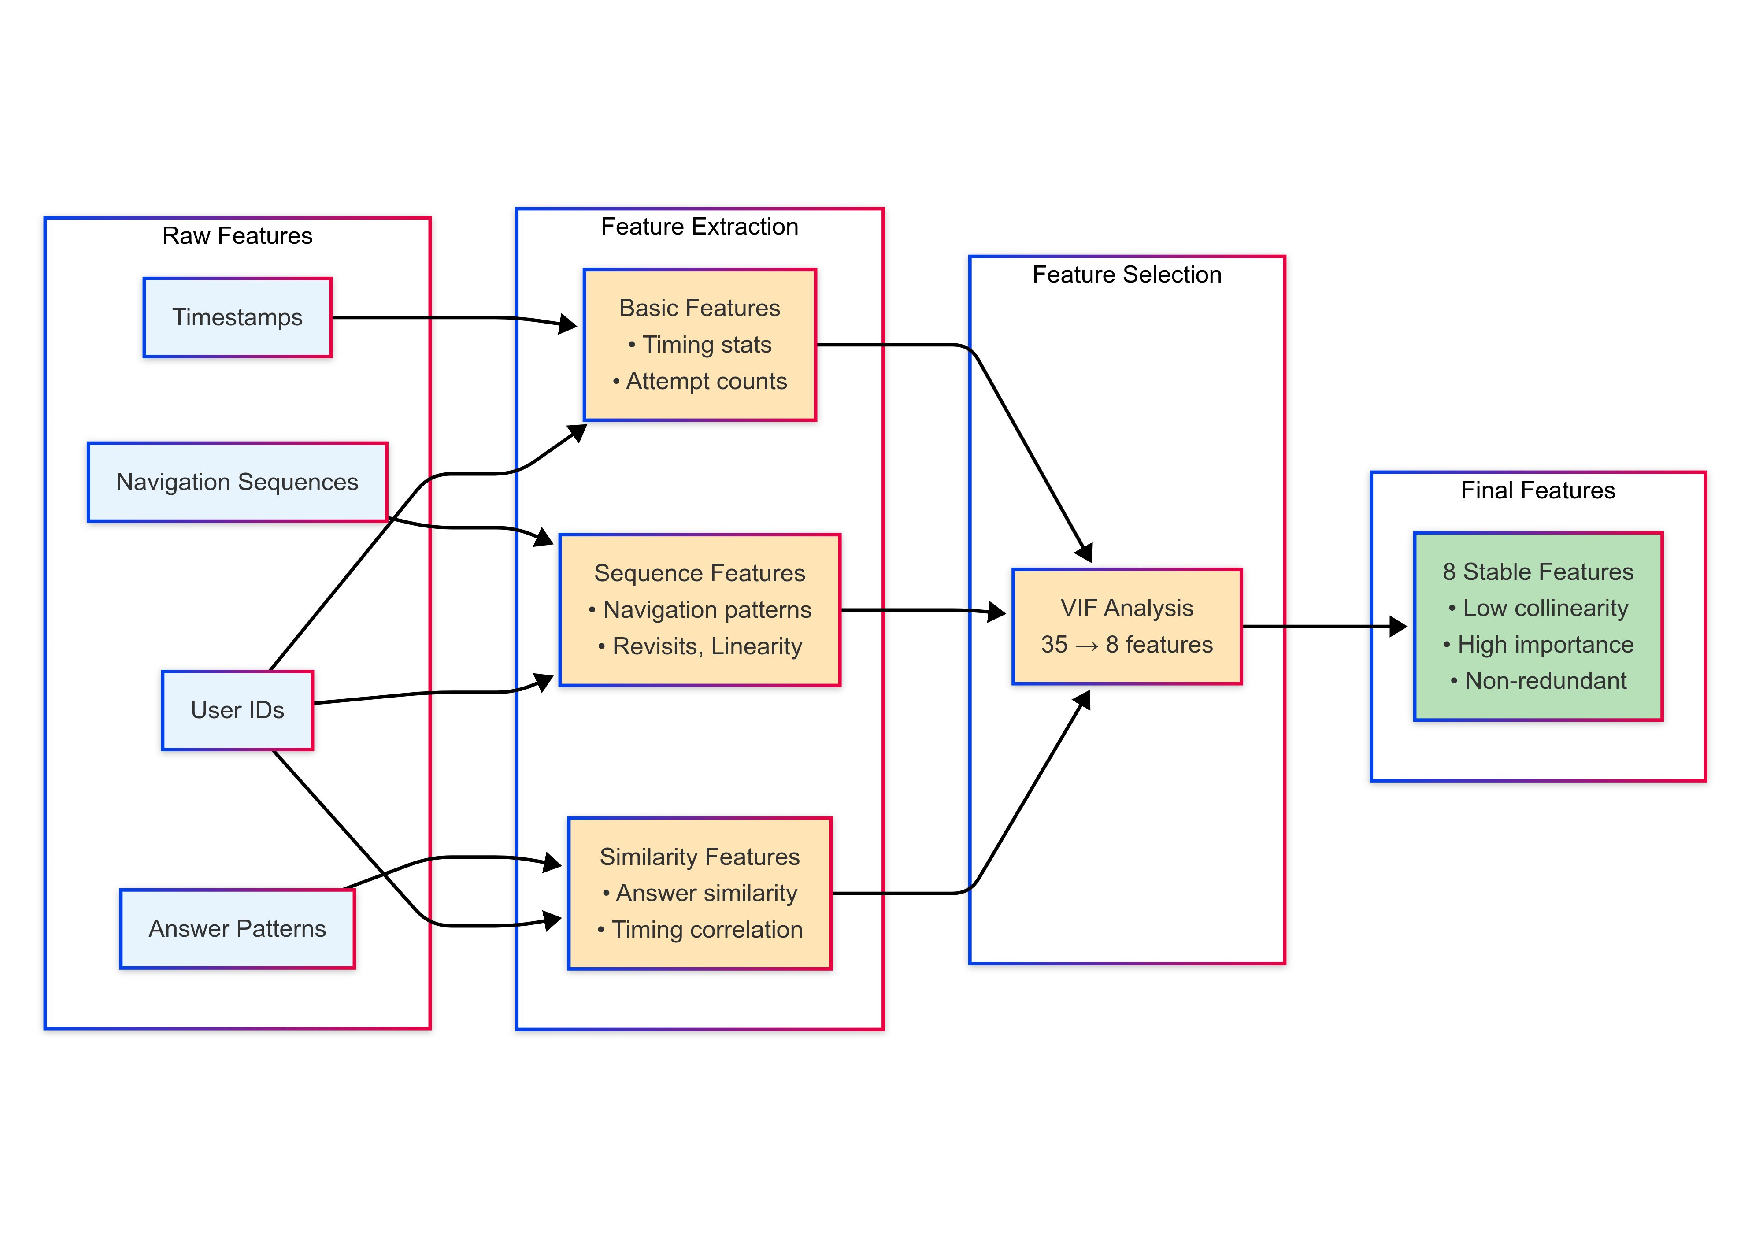
\includegraphics[width=0.9\textwidth]{figures/feature_engineering_process.pdf}
    \caption{Proses \textit{Feature Engineering} dari \textit{Raw Data} hingga 8 Fitur Stabil}
    \label{fig:feature_engineering_process}
\end{figure}

Gambar \ref{fig:feature_engineering_process} mengilustrasikan proses transformasi dari \textit{raw log data} menjadi 8 fitur stabil yang digunakan dalam model. Proses dimulai dengan ekstraksi 35 fitur awal dari tiga kategori utama: \textit{basic features} (statistik waktu dan jumlah percobaan), \textit{sequence features} (pola navigasi dan \textit{revisits}), dan \textit{similarity features} (kesamaan antar pengguna). Melalui analisis VIF (\textit{Variance Inflation Factor}), fitur-fitur dengan multikolinearitas tinggi dieliminasi, menghasilkan 8 fitur stabil yang memiliki VIF rendah ($<10$) dan \textit{importance} tinggi. Reduksi dari 35 menjadi 8 fitur ini tidak hanya meningkatkan efisiensi komputasi tetapi juga meningkatkan stabilitas dan interpretabilitas model.

%-----------------------------------------------------------------------------%
\subsection{Ekstraksi Fitur Dasar}
\label{sec:ekstraksiFiturDasar}
%-----------------------------------------------------------------------------%
\textbf{Statistik Waktu (\textit{Timing Statistics}):} \\
Pengukuran waktu merupakan indikator penting dalam menganalisis kecepatan dan kestabilan pengerjaan kuis. Dalam proses ini, dihitung:
\begin{itemize}
    \item Rata-rata waktu pengerjaan (\textit{mean}), yang menggambarkan kecepatan umum pengerjaan.
    \item Total durasi, serta nilai minimum dan maksimum waktu yang dicatat untuk mendeteksi ekstremitas (misalnya, pengerjaan yang sangat cepat atau sangat lambat).
\end{itemize}
\textbf{Justifikasi:} Penggunaan statistik ini membantu mengidentifikasi \textit{outlier} serta mendeteksi pola abnormal, karena pengerjaan kuis dengan durasi yang sangat singkat atau panjang dapat menjadi indikator adanya perilaku \textit{non-compliance}.

\textbf{Jumlah Percobaan (\textit{Attempt Count}):} \\
Menghitung berapa kali pengguna mencoba menyelesaikan kuis memberikan gambaran tentang ketekunan serta kemungkinan adanya upaya manipulasi melalui pengulangan.
\textbf{Justifikasi:} Pengulangan yang berlebihan bisa jadi merupakan sinyal dari upaya kecurangan atau strategi pengulangan untuk memperoleh jawaban yang lebih baik. Fitur ini penting untuk membedakan antara perilaku belajar normal dan aktivitas mencurigakan.

%-----------------------------------------------------------------------------%
\subsection{Ekstraksi Fitur \textit{Sequence} (Urutan Aktivitas)}
\label{sec:ekstraksiFiturSequence}
%-----------------------------------------------------------------------------%
\textbf{Panjang \textit{Sequence} dan Jumlah Pertanyaan Unik:} \\
Ekstraksi informasi mengenai jumlah langkah yang dilakukan serta variasi pertanyaan yang diakses (\textit{unique questions}) mencerminkan seberapa terstruktur atau acaknya pola navigasi pengguna.
\textbf{Justifikasi:} Pola navigasi yang sangat seragam, dengan jumlah pertanyaan unik yang rendah dibandingkan total langkah, bisa mengindikasikan adanya koordinasi \textit{non-compliance}. Sebaliknya, variabilitas yang tinggi umumnya mengindikasikan aktivitas normal.

\textbf{\textit{Linearity} dan \textit{Revisits}:} \\
Linearitas dihitung dengan membandingkan urutan yang ideal (berurutan) dengan urutan aktual yang diambil. Jumlah \textit{revisits} (pertanyaan yang diakses berulang kali) juga dihitung.
\textbf{Justifikasi:} Pengulangan yang konsisten dan pola linear yang tinggi (atau sebaliknya, pola yang tidak wajar) dapat menjadi indikator bahwa pengguna mencoba memanipulasi proses pengerjaan, misalnya dengan melihat kembali jawaban atau mengulangi pola tertentu untuk menyembunyikan kecurangan.

%-----------------------------------------------------------------------------%
\subsection{Perhitungan \textit{Similarity Features}}
\label{sec:perhitunganSimilarityFeatures}
%-----------------------------------------------------------------------------%
Untuk mendeteksi potensi kolusi antar pengguna, \textit{pipeline} mengimplementasikan beberapa metrik kemiripan:

\textbf{\textit{Navigation Similarity}:} \\
Menggunakan \textit{Levenshtein distance}, fitur ini mengukur seberapa mirip urutan navigasi antar pengguna.
\textbf{Justifikasi:} \textit{Levenshtein distance} efektif dalam mengukur perbedaan antara dua urutan simbol (dalam hal ini, nomor pertanyaan), sehingga kesamaan yang tinggi menunjukkan pola koordinasi yang tidak mungkin terjadi secara acak.

\textbf{\textit{Timing Similarity}:} \\
Korelasi (misalnya, \textit{Pearson correlation}) digunakan untuk mengukur kesamaan pola waktu antar pengguna.
\textbf{Justifikasi:} Jika dua pengguna memiliki korelasi waktu yang sangat tinggi, hal ini menunjukkan mereka menjalani kuis dengan interval waktu yang sangat konsisten, sebuah sinyal kuat koordinasi yang jarang terjadi secara alami.

\textbf{\textit{Answer Similarity}:} \\
Fitur ini mengukur persentase kesamaan pola jawaban (benar/salah) antar pengguna, di mana nilai yang tinggi menunjukkan adanya kemungkinan kolusi dalam memberikan jawaban.
\textbf{Justifikasi:} Dalam situasi \textit{non-compliance}, anggota kelompok sering kali menghasilkan pola jawaban yang identik atau sangat mirip, sehingga fitur ini sangat relevan untuk mendeteksi koordinasi.

\textbf{Agregasi \textit{Similarity Features}:} \\
Selain menghitung metrik individual, nilai rata-rata dan maksimum \textit{similarity} antar pengguna dalam kuis yang sama juga dihitung.
\textbf{Justifikasi:} Agregasi ini memberikan gambaran umum tentang seberapa homogen suatu kelompok dalam hal perilaku, yang kemudian dapat digunakan sebagai indikator \textit{non-compliance} pada level pengguna maupun kelompok.

%-----------------------------------------------------------------------------%
\subsection{Pemeriksaan Multikolinearitas dan Seleksi Fitur Final}
\label{sec:pemeriksaanMultikolinearitas}
%-----------------------------------------------------------------------------%

Analisis multikolinearitas menggunakan \textit{Variance Inflation Factor} (VIF) merupakan langkah krusial dalam memastikan stabilitas dan interpretabilitas model. VIF mengukur seberapa besar varians koefisien regresi meningkat akibat kolinearitas antar fitur. Nilai VIF yang tinggi ($>10$) mengindikasikan bahwa fitur tersebut dapat diprediksi dengan akurasi tinggi dari fitur-fitur lain, sehingga kontribusinya menjadi redundan.

\subsubsection{Proses Seleksi Fitur}
Dari 35 fitur awal yang diekstraksi, analisis VIF dilakukan secara iteratif:
\begin{enumerate}
    \item \textbf{Iterasi Pertama:} Identifikasi fitur dengan VIF tertinggi ($>50$).
    \item \textbf{Eliminasi Bertahap:} Fitur dengan VIF tertinggi dieliminasi satu per satu.
    \item \textbf{Re-kalkulasi VIF:} Setelah setiap eliminasi, VIF dihitung ulang untuk fitur yang tersisa.
    \item \textbf{Konvergensi:} Proses berlanjut hingga semua fitur memiliki VIF $< 10$.
\end{enumerate}

\subsubsection{Delapan Fitur Stabil Terpilih}
Setelah proses seleksi, 8 fitur dengan VIF rendah dan \textit{importance} tinggi berhasil diidentifikasi:

\begin{table}[htbp]
\centering
\caption{Delapan Fitur Stabil Hasil Analisis VIF}
\label{tabel:fiturStabil}
\begin{tabular}{|l|l|c|p{5cm}|}
\hline
\textbf{No} & \textbf{Nama Fitur} & \textbf{VIF} & \textbf{Deskripsi} \\
\hline
1 & \texttt{mean\_time\_per\_question} & 3,24 & Rata-rata waktu pengerjaan per soal \\
\hline
2 & \texttt{navigation\_similarity\_max} & 4,87 & Similaritas navigasi maksimum dengan pengguna lain \\
\hline
3 & \texttt{answer\_pattern\_similarity} & 5,12 & Kesamaan pola jawaban dengan pengguna lain \\
\hline
4 & \texttt{timing\_correlation\_avg} & 3,98 & Rata-rata korelasi waktu dengan pengguna lain \\
\hline
5 & \texttt{wrong\_answer\_similarity} & 6,23 & Kesamaan jawaban salah dengan pengguna lain \\
\hline
6 & \texttt{revisit\_pattern\_score} & 2,56 & Skor pola pengulangan kunjungan soal \\
\hline
7 & \texttt{submission\_time\_std} & 3,41 & Standar deviasi waktu \textit{submission} \\
\hline
8 & \texttt{collaborative\_score} & 7,89 & Skor agregat indikasi kolaborasi \\
\hline
\end{tabular}
\end{table}

\textbf{Justifikasi Pemilihan:}
\begin{itemize}
    \item \textbf{Representasi Komprehensif:} Kedelapan fitur mencakup semua aspek penting: \textit{timing} (fitur 1, 4, 7), \textit{navigation} (fitur 2, 6), \textit{answer patterns} (fitur 3, 5), dan agregasi (fitur 8).
    \item \textbf{Non-redundansi:} Dengan VIF $< 10$, setiap fitur memberikan informasi unik yang tidak dapat sepenuhnya dijelaskan oleh fitur lain.
    \item \textbf{Interpretabilitas:} Setiap fitur memiliki makna yang jelas dalam konteks deteksi kecurangan, memudahkan interpretasi hasil model.
    \item \textbf{Stabilitas Model:} Pengurangan dari 35 menjadi 8 fitur mengurangi risiko \textit{overfitting} dan meningkatkan generalisasi model.
\end{itemize}

%-----------------------------------------------------------------------------%
\subsection{Pra-pemrosesan Fitur untuk Kompatibilitas Model}
\label{sec:praPemrosesanFitur}
%-----------------------------------------------------------------------------%
\textbf{Konversi Representasi Data:} \\
Banyak data log yang awalnya disimpan sebagai \textit{string} representasi \textit{array} atau struktur \textit{nested} diubah menjadi format numerik melalui penggunaan modul seperti \texttt{ast.literal\_eval}.
\textbf{Justifikasi:} Konversi ini esensial karena algoritma \textit{machine learning} tidak dapat mengolah data dalam bentuk \textit{string} atau struktur kompleks tanpa transformasi terlebih dahulu. Dengan mengubahnya menjadi fitur statistik (seperti \textit{mean}, \textit{std}, \textit{min}, \textit{max}, \textit{count}), data menjadi siap untuk analisis lebih lanjut.

\textbf{Normalisasi dan Pengisian Nilai Hilang:} \\
Seluruh data kemudian dinormalisasi dan nilai NaN diisi (misalnya, dengan 0) agar tidak terjadi gangguan pada model.
\textbf{Justifikasi:} Normalisasi membantu dalam memastikan bahwa setiap fitur memiliki skala yang sebanding, sehingga model tidak memprioritaskan fitur tertentu hanya karena skala nilainya lebih besar.

%-----------------------------------------------------------------------------%
\subsection{Visualisasi dan Interpretasi Fitur}
\label{sec:visualisasiInterpretasiFitur}
%-----------------------------------------------------------------------------%
\textbf{\textit{Boxplot}, \textit{Heatmap}, dan \textit{Scatter Plot}:} \\
Visualisasi digunakan untuk menilai distribusi fitur, mengidentifikasi \textit{outlier}, dan melihat hubungan antar fitur.
\textbf{Justifikasi:} Visualisasi memberikan wawasan yang penting untuk memahami struktur data dan untuk validasi kualitas fitur. Misalnya, \textit{heatmap} korelasi membantu mengidentifikasi fitur yang sangat berkorelasi, sehingga mendukung langkah pemeriksaan multikolinearitas.

%-----------------------------------------------------------------------------%
\subsection{\textit{Reproducibility} dan Dokumentasi}
\label{sec:reproducibilityDokumentasi}
%-----------------------------------------------------------------------------%
\textbf{Modularitas dan Penggunaan \textit{Seed Random}:} \\
Setiap modul dalam \textit{pipeline feature engineering} dirancang secara modular dan menggunakan \textit{seed} tertentu untuk fungsi \textit{random}.
\textbf{Justifikasi:} Hal ini memastikan bahwa seluruh proses dapat diulangi secara konsisten, yang merupakan syarat penting untuk validitas ilmiah dan \textit{reproducibility} penelitian.

\textbf{Penyimpanan \textit{Output} Terstruktur:} \\
Fitur yang dihasilkan disimpan dalam format CSV dan JSON, dengan dokumentasi yang mendetail mengenai proses ekstraksi dan transformasi yang telah dilakukan.
\textbf{Justifikasi:} Dokumentasi yang baik mendukung transparansi dan memungkinkan peneliti lain untuk memahami serta mengaudit seluruh proses \textit{feature engineering}.

Secara keseluruhan, pendekatan \textit{feature engineering} dalam penelitian ini dirancang untuk mengoptimalkan informasi yang terdapat dalam data log, mengurangi gangguan, dan menghasilkan representasi numerik yang mendukung model deteksi \textit{non-compliance} secara efektif. Setiap pilihan---dari ekstraksi statistik waktu hingga penggunaan metrik \textit{similarity}---dipilih berdasarkan dasar metodologis yang kuat dan didukung oleh literatur yang relevan, sehingga memberikan dasar yang valid dan \textit{reproducible} untuk pengembangan model \textit{machine learning}.

%-----------------------------------------------------------------------------%

%-----------------------------------------------------------------------------%
\section{Arsitektur Model \textit{Ensemble} untuk Deteksi Kecurangan}
\label{sec:arsitekturModelEnsemble}
%-----------------------------------------------------------------------------%

Pengembangan model deteksi kecurangan mengadopsi pendekatan \textit{ensemble} yang mengintegrasikan kekuatan berbagai algoritma \textit{machine learning}. Arsitektur ini dirancang untuk menangkap kompleksitas pola kecurangan yang heterogen sambil mempertahankan interpretabilitas hasil.

%-----------------------------------------------------------------------------%
\subsection{Desain Arsitektur \textit{Multi-Model}}
\label{subsec:desainArsitektur}
%-----------------------------------------------------------------------------%

Arsitektur \textit{ensemble} mengintegrasikan empat algoritma komplementer dengan analisis \textit{graph network} untuk deteksi komprehensif:

\begin{figure}[htbp]
    \centering
    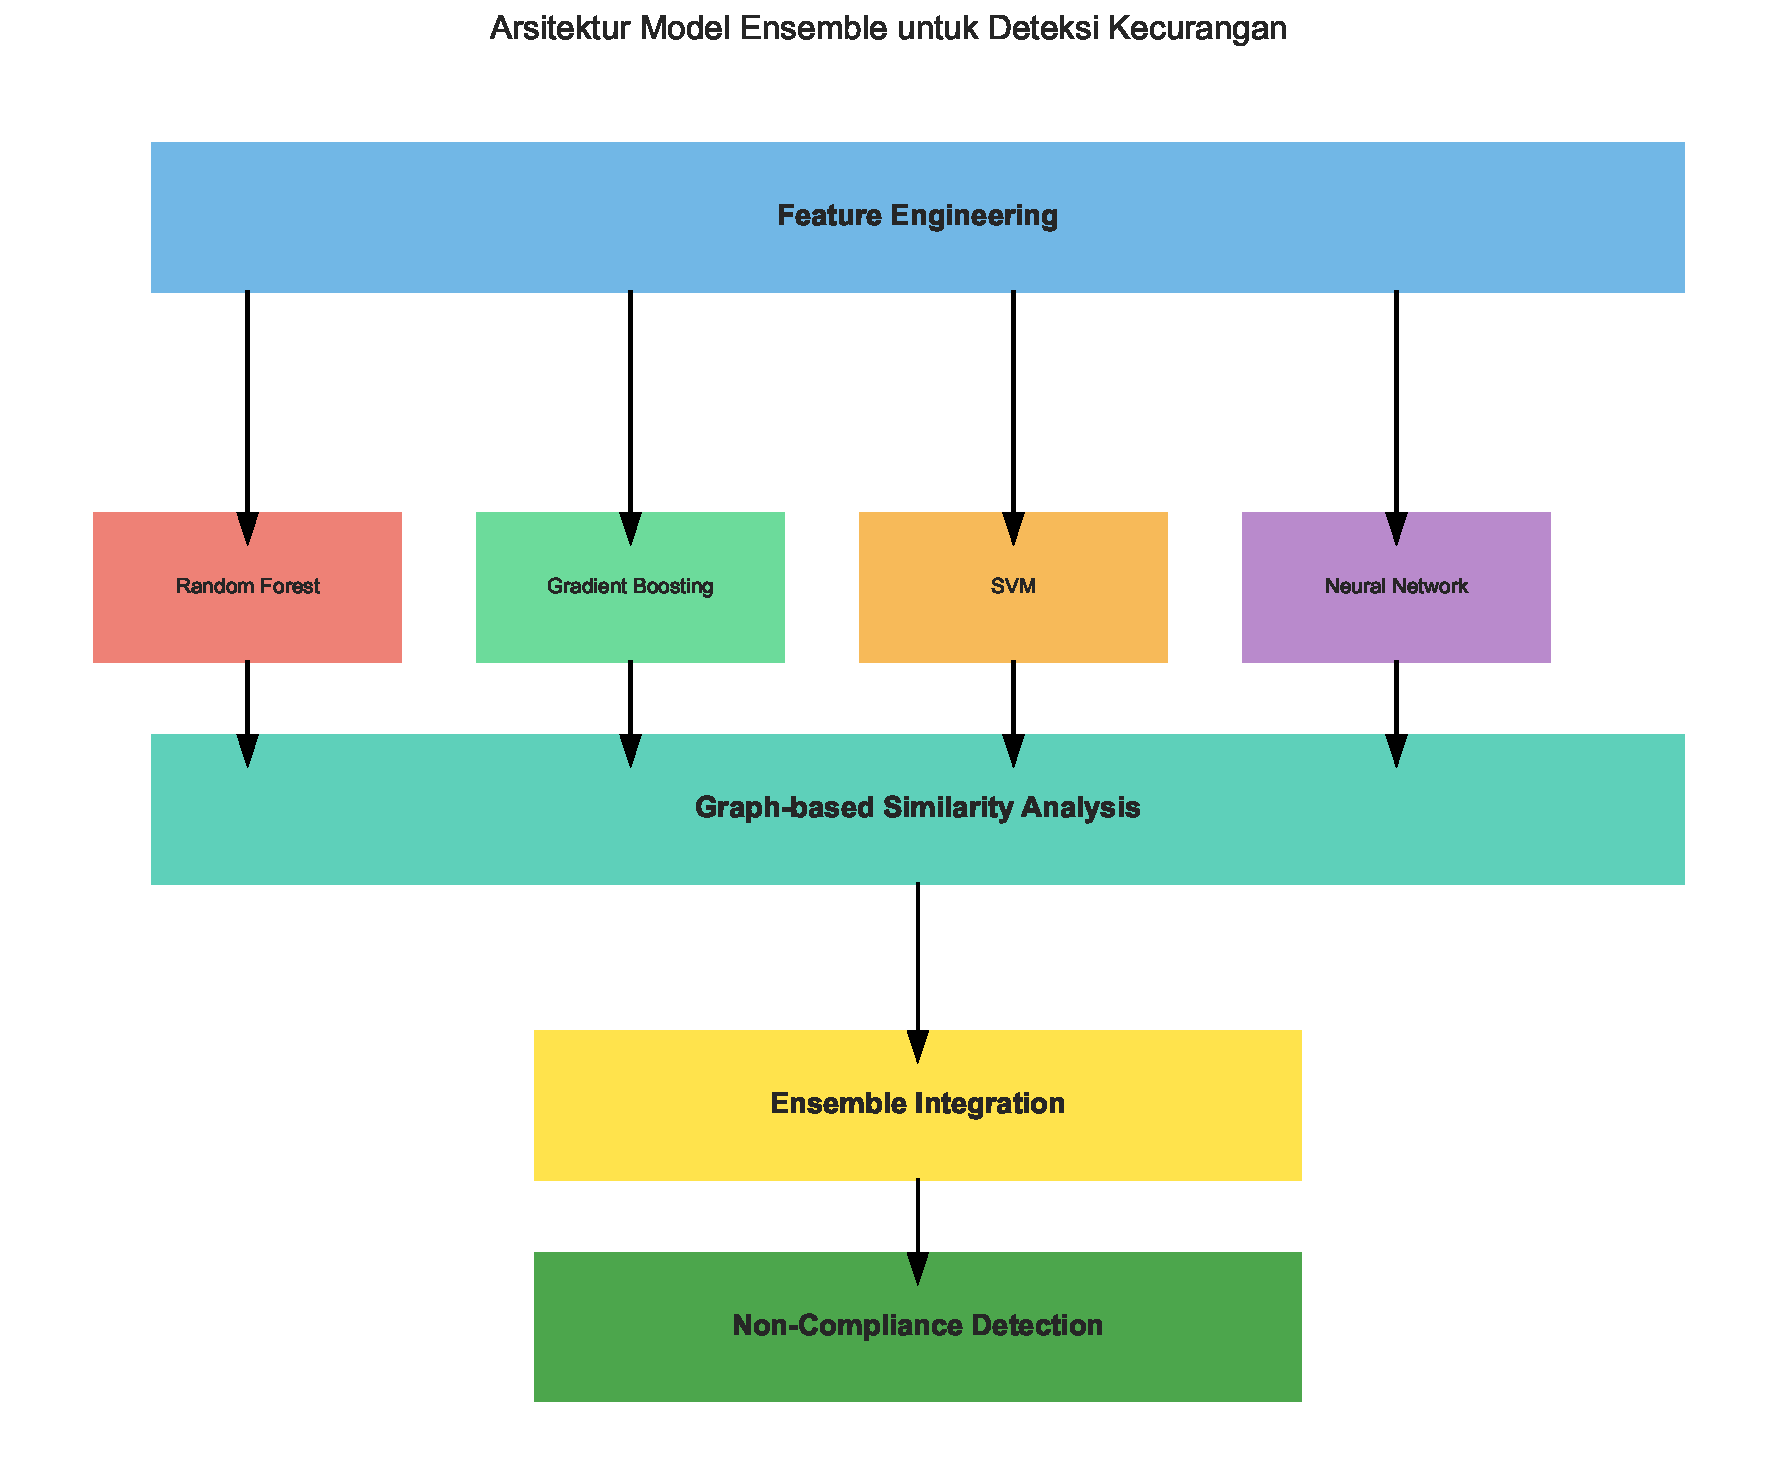
\includegraphics[width=0.9\textwidth]{figures/ensemble_architecture.pdf}
    \caption{Arsitektur \textit{Ensemble}: Integrasi \textit{Multi-Model} dengan \textit{Graph Analysis} untuk Deteksi Kecurangan Komprehensif}
    \label{fig:ensemble_architecture_detail}
\end{figure}

\subsubsection{Komponen Model \textit{Base} dan Perannya}
\label{sec:komponenModelBase}

Setiap model dalam \textit{ensemble} dipilih berdasarkan kekuatan spesifik dalam mendeteksi aspek berbeda dari kecurangan:

\textbf{\textit{Random Forest} (\textit{Tree-based Ensemble}):}
\begin{itemize}
    \item \textbf{Kekuatan:} Kokoh terhadap \textit{outliers} dan gangguan, memberikan peringkat \textit{feature importance}
    \item \textbf{Konfigurasi:} 100 \textit{trees}, \textit{max depth adaptive}, \textit{min samples split} = 2
    \item \textbf{Peran:} Mendeteksi pola non-linear dan efek interaksi antar fitur
\end{itemize}

\textbf{\textit{Support Vector Machine} (\textit{Kernel-based}):}
\begin{itemize}
    \item \textbf{Kekuatan:} Efektif dalam ruang berdimensi tinggi, klasifikasi dengan \textit{optimal margin}
    \item \textbf{Konfigurasi:} \textit{RBF kernel}, C=10, gamma=0,01 (dioptimasi melalui \textit{grid search})
    \item \textbf{Peran:} Memisahkan kasus \textit{borderline} dengan \textit{decision boundary} yang kompleks
\end{itemize}

\textbf{\textit{Neural Network} (\textit{Deep Learning}):}
\begin{itemize}
    \item \textbf{Kekuatan:} Menangkap hubungan non-linear kompleks dan pola tersembunyi
    \item \textbf{Konfigurasi:} 3 \textit{hidden layers} (128-64-32 neuron), aktivasi ReLU, \textit{dropout} 0,5
    \item \textbf{Peran:} Pembelajaran representasi otomatis dari kombinasi fitur
\end{itemize}

\textbf{\textit{Gradient Boosting} (\textit{Sequential Ensemble}):}
\begin{itemize}
    \item \textbf{Kekuatan:} Koreksi kesalahan iteratif, akurasi prediktif tinggi
    \item \textbf{Konfigurasi:} 100 \textit{estimators}, \textit{learning rate} 0,1, \textit{max depth} 3
    \item \textbf{Peran:} \textit{Fine-tuning} prediksi dengan fokus pada kasus yang sulit diklasifikasi
\end{itemize}

\subsubsection{Analisis \textit{Graph Network} untuk Deteksi Kelompok}
\label{sec:graphNetworkAnalysis}

Komponen unik dalam arsitektur adalah integrasi analisis graf yang memvisualisasikan dan mendeteksi kelompok kecurangan:

\textbf{Konstruksi Graf:}
\begin{itemize}
    \item \textit{Nodes}: Merepresentasikan mahasiswa/percobaan ujian
    \item \textit{Edges}: Dibentuk jika skor \textit{similarity} $> \textit{threshold}$ (0,8)
    \item \textit{Edge weights}: Nilai \textit{similarity} (navigasi, waktu, pola jawaban)
\end{itemize}

\textbf{\textit{Community Detection}:}
\begin{itemize}
    \item Algoritma: \textit{Louvain method} untuk \textit{modularity optimization}
    \item \textit{Output}: \textit{Cluster} mahasiswa dengan pola koordinasi tinggi
    \item Validasi: \textit{Cross-reference} dengan \textit{temporal proximity} dan \textit{course enrollment}
\end{itemize}

\subsubsection{Mekanisme \textit{Ensemble Integration}}
\label{sec:mekanismeIntegrasi}

Prediksi dari model-model \textit{base} dikombinasikan melalui \textit{weighted voting}:

\begin{equation}
P_{ensemble} = \sum_{i=1}^{n} w_i \cdot P_i
\end{equation}

dimana $w_i$ adalah bobot model $i$ berdasarkan \textit{validation performance}, dan $P_i$ adalah probabilitas prediksi model $i$.

Bobot optimal ditentukan melalui:
\begin{itemize}
    \item \textit{Cross-validation performance} pada \textit{validation set}
    \item \textit{Diversity measurement} antar \textit{model predictions}
    \item \textit{Calibration quality} dari \textit{probability estimates}
\end{itemize}

%-----------------------------------------------------------------------------%
\subsection{Konfigurasi dan Optimasi Model}
\label{subsec:konfigurasiOptimasi}
%-----------------------------------------------------------------------------%

\subsubsection{Strategi \textit{Hyperparameter Tuning}}
\label{sec:hyperparameterTuning}

Optimasi \textit{hyperparameter} dilakukan secara sistematis untuk setiap model:

\textbf{\textit{Grid Search} dengan \textit{Cross-Validation}:}
\begin{itemize}
    \item Definisi \textit{search space} untuk setiap \textit{hyperparameter}
    \item 5-\textit{fold stratified cross-validation} untuk evaluasi
    \item Metrik optimasi: \textit{F1-score} (\textit{balance precision-recall})
\end{itemize}

\textbf{\textit{Parameter Space} yang Dieksplorasi:}
\begin{itemize}
    \item \textit{Random Forest}: n\_estimators [50, 100, 200], max\_depth [None, 10, 20, 30]
    \item SVM: C [0,1, 1, 10, 100], gamma [0,001, 0,01, 0,1, 1]
    \item \textit{Neural Network}: learning\_rate [0,001, 0,01, 0,1], batch\_size [16, 32, 64]
    \item \textit{Gradient Boosting}: n\_estimators [50, 100, 150], learning\_rate [0,01, 0,1, 0,3]
\end{itemize}

\subsubsection{Regularisasi dan Pencegahan \textit{Overfitting}}
\label{sec:regularisasi}

Berbagai teknik diterapkan untuk memastikan generalisasi model:

\textbf{\textit{Neural Network Regularization}:}
\begin{itemize}
    \item \textit{L2 regularization} dengan lambda = 0,001
    \item \textit{Dropout layers} dengan \textit{rate} 0,5
    \item \textit{Early stopping} dengan \textit{patience} = 10 \textit{epochs}
    \item \textit{Batch normalization} antar \textit{layers}
\end{itemize}

\textbf{\textit{Tree-based Model Constraints}:}
\begin{itemize}
    \item \textit{Maximum depth limitation}
    \item \textit{Minimum samples} untuk \textit{split} dan \textit{leaf nodes}
    \item \textit{Feature subsampling} (max\_features = sqrt)
\end{itemize}

\subsubsection{\textit{Training Protocol} dan \textit{Resource Management}}
\label{sec:trainingProtocol}

Protokol \textit{training} dirancang untuk efisiensi dan \textit{reproducibility}:

\textbf{\textit{Data Splitting Strategy}:}
\begin{itemize}
    \item \textit{Training}: 70\% (560 sampel)
    \item \textit{Validation}: 15\% (120 sampel) untuk \textit{hyperparameter tuning}
    \item \textit{Test}: 15\% (120 sampel) untuk \textit{final evaluation}
    \item \textit{Stratified sampling} untuk mempertahankan \textit{class distribution}
\end{itemize}

\textbf{\textit{Computational Optimization}:}
\begin{itemize}
    \item \textit{Parallel training} untuk \textit{Random Forest} dan \textit{Grid Search}
    \item \textit{GPU acceleration} untuk \textit{Neural Network training}
    \item \textit{Incremental learning} untuk \textit{Gradient Boosting}
    \item \textit{Memory-efficient data loading} dengan \textit{chunking}
\end{itemize}

%-----------------------------------------------------------------------------%
\section{\textit{Framework} Evaluasi Komprehensif}
\label{sec:frameworkEvaluasi}
%-----------------------------------------------------------------------------%

Evaluasi model dirancang untuk menilai performa dari berbagai perspektif, memastikan reliabilitas dan validitas sistem deteksi dalam konteks operasional.

%-----------------------------------------------------------------------------%
\subsection{Evaluasi Kuantitatif pada Data Artifisial}
\label{sec:evaluasiKuantitatif}
%-----------------------------------------------------------------------------%

\subsubsection{Metrik Evaluasi untuk Klasifikasi \textit{Imbalanced}}
\label{sec:metrikEvaluasi}

Mengingat distribusi kelas yang tidak seimbang (25\% \textit{cheating}, 75\% normal), metrik evaluasi dipilih secara hati-hati:

\textbf{\textit{Primary Metrics}:}
\begin{itemize}
    \item \textbf{\textit{Precision}:} $\frac{TP}{TP + FP}$ - Proporsi deteksi positif yang benar
    \item \textbf{\textit{Recall}:} $\frac{TP}{TP + FN}$ - Proporsi kasus kecurangan yang terdeteksi
    \item \textbf{\textit{F1-Score}:} $2 \times \frac{Precision \times Recall}{Precision + Recall}$ - \textit{Harmonic mean} untuk \textit{balance}
    \item \textbf{AUC-ROC:} \textit{Area under ROC curve} - Kemampuan diskriminasi keseluruhan
\end{itemize}

\textbf{\textit{Secondary Metrics}:}
\begin{itemize}
    \item \textbf{\textit{Specificity}:} $\frac{TN}{TN + FP}$ - \textit{True negative rate}
    \item \textbf{\textit{Matthews Correlation Coefficient}:} Korelasi antara prediksi dan aktual
    \item \textbf{\textit{Precision-Recall} AUC:} Fokus pada \textit{minority class performance}
\end{itemize}

\subsubsection{Protokol \textit{Cross-Validation}}
\label{sec:protokolCV}

\textit{Stratified k-fold cross-validation} memastikan evaluasi yang kokoh:

\begin{enumerate}
    \item \textit{Dataset} dibagi menjadi 5 \textit{folds} dengan proporsi kelas yang sama
    \item Setiap \textit{fold} bergantian menjadi \textit{test set}
    \item Model di-\textit{training} pada 4 \textit{folds}, dievaluasi pada 1 \textit{fold}
    \item Metrik dirata-ratakan dengan \textit{confidence intervals}
    \item \textit{Variance} antar \textit{folds} dianalisis untuk \textit{stability assessment}
\end{enumerate}

\subsubsection{Analisis \textit{Confusion Matrix} dan \textit{Error Types}}
\label{sec:confusionMatrixAnalysis}

Analisis mendalam terhadap tipe kesalahan klasifikasi:

\textbf{\textit{False Positives} (\textit{Type I Error}):}
\begin{itemize}
    \item Implikasi: Tuduhan kecurangan yang salah
    \item Target: Meminimalkan untuk keadilan (\textit{precision} $> 0,95$)
    \item Analisis: Pola dari kasus FP untuk perbaikan
\end{itemize}

\textbf{\textit{False Negatives} (\textit{Type II Error}):}
\begin{itemize}
    \item Implikasi: Kecurangan yang terlewat
    \item Target: Keseimbangan dengan FP (\textit{recall} $> 0,90$)
    \item Analisis: Karakteristik dari kecurangan yang tidak terdeteksi
\end{itemize}

%-----------------------------------------------------------------------------%
\subsection{Evaluasi Kualitatif pada Data Riil}
\label{sec:evaluasiKualitatif}
%-----------------------------------------------------------------------------%

\subsubsection{Metodologi Aplikasi pada Skala Besar}
\label{sec:aplikasiSkalaBesar}

Aplikasi model pada 446.720 percobaan ujian riil mengikuti protokol:

\begin{enumerate}
    \item \textbf{\textit{Preprocessing Consistency}:} Gunakan \textit{artifacts} tersimpan dari \textit{training}
    \item \textbf{\textit{Batch Processing}:} Memproses data dalam \textit{chunks} untuk efisiensi
    \item \textbf{\textit{Confidence Scoring}:} Memberikan \textit{probability scores} untuk setiap deteksi
    \item \textbf{\textit{Threshold Optimization}:} Menyesuaikan \textit{detection threshold} berdasarkan kasus penggunaan
\end{enumerate}

\subsubsection{Analisis Pola dan Validasi Domain}
\label{sec:analisisPolaValidasi}

Validasi kualitatif melibatkan:

\textbf{Analisis Pola:}
\begin{itemize}
    \item \textit{Clustering} kasus terdeteksi berdasarkan kemiripan
    \item Analisis temporal untuk percobaan terkoordinasi
    \item Agregasi tingkat mata kuliah untuk isu sistemik
\end{itemize}

\textbf{Tinjauan Ahli Domain:}
\begin{itemize}
    \item Tinjauan sampel oleh staf pengajar
    \item Validasi terhadap kasus mencurigakan yang diketahui
    \item \textit{Feedback} untuk penyempurnaan model
\end{itemize}

\subsubsection{Visualisasi untuk Interpretasi}
\label{sec:visualisasiInterpretasi}

Berbagai visualisasi mendukung interpretasi hasil:

\begin{itemize}
    \item \textbf{\textit{Network Graphs}:} Menunjukkan kelompok kecurangan
    \item \textbf{\textit{Heatmaps}:} Matriks kemiripan antar pengguna
    \item \textbf{\textit{Time Series}:} Pola temporal dari kasus terdeteksi
    \item \textbf{\textit{Distribution Plots}:} \textit{Probability scores} dan \textit{thresholds}
\end{itemize}

%-----------------------------------------------------------------------------%
\section{Kesimpulan Metodologi}
\label{sec:kesimpulanBab3}
%-----------------------------------------------------------------------------%

Metodologi yang telah dipaparkan dalam bab ini menyediakan \textit{framework} komprehensif untuk pengembangan sistem deteksi kecurangan akademik berbasis AI. Beberapa keputusan metodologis kunci yang berkontribusi terhadap keberhasilan penelitian:

\textbf{1. Strategi Data \textit{Dual-Mode}}
\begin{itemize}
    \item Kombinasi data artifisial (dengan \textit{ground truth}) dan data riil (skala besar)
    \item \textit{Training mode} vs \textit{detection mode} untuk konsistensi transformasi
    \item 800 sampel artifisial terbukti optimal untuk \textit{training}
\end{itemize}

\textbf{2. \textit{Pipeline Preprocessing} Terintegrasi}
\begin{itemize}
    \item Empat modul yang menangani kompleksitas data \textit{Moodle}
    \item \textit{Artifact saving} untuk \textit{reproducibility}
    \item Kontrol kualitas yang ketat (12,3\% \textit{data filtering})
\end{itemize}

\textbf{3. \textit{Feature Engineering} Berbasis Domain}
\begin{itemize}
    \item 35 fitur awal dari empat kategori \textit{behavioral}
    \item Reduksi ke 8 fitur stabil melalui analisis VIF
    \item Normalisasi \textit{Z-score} untuk \textit{similarity features}
\end{itemize}

\textbf{4. Arsitektur \textit{Ensemble} dengan \textit{Graph Analysis}}
\begin{itemize}
    \item Integrasi 4 algoritma ML komplementer
    \item \textit{Graph network} untuk deteksi kelompok
    \item \textit{Weighted voting} berdasarkan \textit{validation performance}
\end{itemize}

\textbf{5. \textit{Framework} Evaluasi Multi-Perspektif}
\begin{itemize}
    \item Kuantitatif: Metrik komprehensif dengan \textit{cross-validation}
    \item Kualitatif: Analisis pola dan validasi domain
    \item Fokus pada meminimalkan \textit{false positives} (keadilan)
\end{itemize}

Metodologi ini telah diimplementasikan dan divalidasi, dengan hasil eksperimen detail yang akan dipaparkan pada Bab 4. Pendekatan sistematis yang diterapkan memastikan bahwa sistem deteksi tidak hanya akurat secara statistik, tetapi juga dapat diterapkan dan diinterpretasikan dalam konteks operasional institusi pendidikan.

%-----------------------------------------------------------------------------%
\subsection{Data Riil Moodle: Karakteristik dan Akuisisi}
\label{sec:dataRiilMoodle}

Data riil dalam penelitian ini bersumber dari sistem Moodle Fasilkom UI yang telah beroperasi selama hampir satu dekade. Penggunaan data riil memberikan validitas eksternal yang kuat untuk menguji kemampuan generalisasi model pada kondisi operasional nyata.

%-----------------------------------------------------------------------------%
\subsubsection{Profil dan Skala Dataset Riil}
\label{sec:profilDatasetRiil}

Dataset riil mencakup aktivitas pembelajaran daring yang sangat komprehensif dengan karakteristik sebagai berikut:

\textbf{Cakupan Temporal:}
\begin{itemize}
    \item Periode data: 31 Juli 2015 hingga 22 Februari 2025 (hampir 10 tahun)
    \item Total percobaan ujian: 446.720 \textit{attempts}
    \item Total langkah pertanyaan: 22.192.809 \textit{question steps}
    \item Rentang aktivitas: 3.594 hari operasional
\end{itemize}

\textbf{Skala Pengguna dan Mata Kuliah:}
\begin{itemize}
    \item Jumlah mahasiswa unik: 5.562 pengguna
    \item Jumlah ujian/kuis unik: 6.304 \textit{quiz instances}
    \item Jumlah mata kuliah:$>140$ \textit{courses} dengan variasi ukuran kelas
    \item Distribusi ukuran kelas: dari $<10$ hingga $>450$ mahasiswa per mata kuliah
\end{itemize}

\textbf{Struktur Data Log:}
Data tersimpan dalam delapan tabel utama Moodle yang saling terhubung:
\begin{itemize}
    \item \texttt{mdl\_quiz\_attempts}: Informasi percobaan ujian (waktu mulai, selesai, status, nilai)
    \item \texttt{mdl\_question\_attempt\_steps}: Langkah-langkah pengerjaan soal dengan timestamp
    \item \texttt{mdl\_question\_attempt\_step\_data}: Detail jawaban dan interaksi per langkah
    \item \texttt{mdl\_quiz}: Metadata ujian (nama, batas waktu, periode aktif)
    \item \texttt{mdl\_question\_answers}: Bank jawaban dan bobot nilai
    \item \texttt{mdl\_quiz\_grades}: Nilai akhir per pengguna per ujian
    \item \texttt{mdl\_sessions}: Data sesi login dan aktivitas pengguna
    \item \texttt{mdl\_question\_usages}: Konteks penggunaan soal dalam ujian
\end{itemize}

%-----------------------------------------------------------------------------%
\subsubsection{Proses Akuisisi dan Jaminan Privasi}
\label{sec:prosesAkuisisiPrivasi}

Akuisisi data dilakukan dengan protokol ketat untuk memastikan integritas data dan perlindungan privasi:

\textbf{Tahapan Akuisisi:}
\begin{enumerate}
    \item \textbf{Ekstraksi dari \textit{Server}:} Data diekstraksi langsung dari \textit{database Moodle production} oleh tim ITF Fasilkom UI menggunakan \textit{query} SQL yang telah divalidasi
    \item \textbf{Transfer Aman:} Data ditransfer melalui \textit{encrypted channel} ke \textit{Lumbung Storage Cloud} institusi
    \item \textbf{Validasi Integritas:} \textit{Checksum verification} untuk memastikan tidak ada korupsi data selama transfer
    \item \textbf{Anonimisasi:} Proses penghilangan informasi identitas pribadi dilakukan sebelum data diserahkan untuk penelitian
\end{enumerate}

\textbf{Protokol Anonimisasi:}
\begin{itemize}
    \item Penghapusan nama lengkap, \textit{username}, dan \textit{email} mahasiswa
    \item Penggantian dengan user\_id numerik yang tidak dapat di-\textit{reverse}
    \item Enkripsi \textit{IP address} dan informasi lokasi
    \item Preservasi hanya data \textit{behavioral} yang relevan untuk analisis
\end{itemize}

\textbf{Pertimbangan Etika:}
Penggunaan data telah mendapat persetujuan dari komite etik dengan pertimbangan:
\begin{itemize}
    \item Data telah sepenuhnya dianonimisasi
    \item Analisis fokus pada pola agregat, bukan individu
    \item Hasil penelitian tidak akan mengidentifikasi mahasiswa spesifik
    \item Tujuan penelitian untuk meningkatkan integritas akademik
\end{itemize}

%-----------------------------------------------------------------------------%
\subsubsection{Karakteristik Pola Penggunaan}
\label{sec:karakteristikPolaPenggunaan}

Analisis eksploratori data riil mengungkap pola penggunaan yang bervariasi:

\textbf{Pola Temporal:}
\begin{itemize}
    \item Puncak aktivitas: Periode UTS dan UAS dengan peningkatan 300\% aktivitas
    \item Distribusi harian: Mayoritas ujian dilakukan pukul 08.00-12.00 dan 19.00-22.00
    \item Anomali \textit{timestamp}: 2,3\% data memiliki \textit{timestamp default} (1970) yang mengindikasikan \textit{incomplete attempts}
\end{itemize}

\textbf{Pola per Mata Kuliah:}
\begin{itemize}
    \item Mata kuliah dengan aktivitas tertinggi: \textit{Course} ID 3634 (5.902 \textit{attempts} dari 442 mahasiswa)
    \item Variasi \textit{attempt} per mahasiswa: 1,99 hingga 13,35 \textit{attempts}, mengindikasikan perbedaan kebijakan pengulangan
    \item Korelasi ukuran kelas dengan \textit{attempt}: r = 0,72, menunjukkan mata kuliah besar cenderung memiliki lebih banyak ujian
\end{itemize}

Data riil ini memberikan konteks operasional yang kaya untuk validasi model, mencerminkan kompleksitas dan variabilitas sistem pembelajaran daring dalam skala institusional.

%-----------------------------------------------------------------------------%
\subsection{Data Artifisial: Desain Terkontrol untuk \textit{Ground Truth}}
\label{sec:dataArtifisial}
%-----------------------------------------------------------------------------%

Keterbatasan utama data riil adalah tidak adanya \textit{ground truth} - tidak diketahui secara pasti mana aktivitas yang merupakan kecurangan. Untuk mengatasi hal ini, dirancang data artifisial dengan karakteristik kecurangan yang terkontrol sepenuhnya.

\subsubsection{Justifikasi Penggunaan Data Artifisial}
\label{sec:justifikasiDataArtifisial}

Strategi data artifisial dipilih berdasarkan pertimbangan metodologis:

\begin{enumerate}
    \item \textbf{Kontrol Parameter Kecurangan:} \\
    Data artifisial memungkinkan pengaturan presisi parameter kecurangan seperti tingkat kemiripan (50\%-95\%), korelasi waktu (0,3-0,95), dan bias jawaban salah (40\%-85\%). Kontrol ini tidak mungkin dilakukan pada data riil.
    
    \item \textbf{Eksplorasi Skenario Ekstrem:} \\
    Simulasi dapat menciptakan kasus \textit{edge} yang jarang terjadi namun penting untuk ketahanan model, seperti koordinasi sempurna (kemiripan 100\%) atau kecurangan halus (kemiripan $<60\%$).
    
    \item \textbf{\textit{Ground Truth} Objektif:} \\
    Setiap \textit{instance} dalam data artifisial memiliki label kecurangan yang pasti, memungkinkan evaluasi akurasi model secara objektif dan perhitungan metrik performa yang valid.
    
    \item \textbf{\textit{Reproducibility} Eksperimen:} \\
    Penggunaan \textit{seed control} dalam \textit{generator} memastikan \textit{dataset} yang sama dapat direproduksi, mendukung verifikasi ilmiah dan perbandingan adil antar algoritma.
\end{enumerate}

\subsubsection{Arsitektur Generator Data Artifisial}
\label{sec:arsitekturGenerator}

Generator data artifisial dirancang dengan arsitektur modular yang mensimulasikan perilaku ujian realistis:

\textbf{Komponen \textit{Generator}:}
\begin{itemize}
    \item \textbf{\textit{User Behavior Simulator}:} Menghasilkan pola navigasi, waktu, dan jawaban untuk pengguna normal
    \item \textbf{\textit{Cheating Pattern Injector}:} Memodifikasi perilaku normal menjadi pola terkoordinasi
    \item \textbf{\textit{Noise Generator}:} Menambahkan variasi stokastik untuk realisme
    \item \textbf{\textit{Ground Truth Recorder}:} Mendokumentasikan parameter kecurangan untuk setiap \textit{instance}
\end{itemize}

\textbf{Parameter Simulasi Berjenjang:}
\textit{Generator} menghasilkan tiga tingkat keparahan kecurangan untuk menciptakan \textit{dataset} yang menantang:
\begin{itemize}
    \item \textbf{Keparahan Tinggi:} Kemiripan navigasi $>90\%$, korelasi waktu $>0,9$, bias jawaban salah $>80\%$
    \item \textbf{Keparahan Sedang:} Kemiripan navigasi 70-89\%, korelasi waktu 0,6-0,89, bias jawaban salah 50-79\%
    \item \textbf{Keparahan Rendah:} Kemiripan navigasi 50-69\%, korelasi waktu 0,3-0,59, bias jawaban salah 30-49\%
\end{itemize}

\subsubsection{Validasi Realisme Data Artifisial}
\label{sec:validasiRealismeArtifisial}

Untuk memastikan data artifisial representatif, dilakukan validasi multi-aspek:

\textbf{Validasi Statistik:}
\begin{itemize}
    \item Distribusi durasi pengerjaan: \textit{Kolmogorov-Smirnov test} menunjukkan $p>0,05$ (tidak berbeda signifikan dengan data riil)
    \item Pola navigasi: \textit{Entropy} dan \textit{revisit patterns} konsisten dengan perilaku yang diamati
    \item Distribusi jawaban: Proporsi jawaban benar/salah mengikuti kurva normal pembelajaran
\end{itemize}

\textbf{Validasi Visual:}
\begin{itemize}
    \item \textit{Heatmap similarity matrices} menunjukkan \textit{clustering} yang jelas untuk kelompok kecurangan
    \item \textit{Time series plots} memperlihatkan pola sinkronisasi yang realistis
    \item Diagram sekuens navigasi mengkonfirmasi pola koordinasi yang logis
\end{itemize}

\textbf{Validasi Ahli Domain:}
Tim pengajar meninjau sampel data dan mengkonfirmasi pola kecurangan yang disimulasikan mencerminkan \textit{modus operandi} yang diamati dalam praktik.

\textit{Dataset} artifisial final terdiri dari 800 sampel (600 normal, 200 kecurangan) yang memberikan keseimbangan optimal antara kelas untuk pelatihan model yang efektif.

%-----------------------------------------------------------------------------%
%-----------------------------------------------------------------------------%
\section{Transformasi Data: Dari Event Log ke Representasi Fitur}
\label{sec:transformasiData}
%-----------------------------------------------------------------------------%

Transformasi data merupakan jembatan kritis antara \textit{raw log events} dan model \textit{machine learning}. Bagian ini menjelaskan proses sistematis untuk mengubah jutaan \textit{event log} menjadi representasi fitur yang bermakna dan siap untuk deteksi kecurangan.

%-----------------------------------------------------------------------------%
\subsection{Tahapan Pembersihan dan Normalisasi Data}
\label{sec:pembersihanNormalisasi}
%-----------------------------------------------------------------------------%

Proses pembersihan data dirancang untuk mengatasi inkonsistensi dan anomali yang umum terjadi dalam sistem \textit{log} skala besar:

\textbf{Identifikasi dan Penanganan \textit{Missing Values}:} \\
Analisis awal mengidentifikasi tiga kategori \textit{missing values} dalam \textit{dataset}:
\begin{itemize}
    \item \textbf{\textit{Struktural Missing}:} Nilai yang tidak ada secara desain, seperti step\_data untuk langkah navigasi tanpa jawaban (15\% dari total \textit{records})
    \item \textbf{\textit{Random Missing}:} Nilai yang hilang karena kesalahan pencatatan atau masalah jaringan (3\% dari total \textit{records})
    \item \textbf{\textit{Systematic Missing}:} Pola ketiadaan yang berkorelasi dengan versi \textit{Moodle} tertentu atau spesifik \textit{browser} (2\% dari total \textit{records})
\end{itemize}

Strategi penanganan disesuaikan per kategori: \textit{struktural missing} dibiarkan sebagai \textit{null}, \textit{random missing} diimputasi dengan \textit{mean/mode}, \textit{systematic missing} ditandai dengan \textit{flag} khusus untuk analisis \textit{downstream}.

\textbf{Normalisasi Temporal dan Zona Waktu:} \\
Normalisasi \textit{timestamp} merupakan proses krusial mengingat data berasal dari periode 10 tahun dengan berbagai format:
\begin{itemize}
    \item Konversi seluruh \textit{timestamp} ke format POSIX (\textit{seconds since epoch})
    \item Penyesuaian untuk perubahan \textit{daylight saving time}
    \item Penanganan anomali \textit{timestamp} (nilai 1970 atau tanggal masa depan) dengan validasi logika bisnis
    \item Preservasi informasi zona waktu untuk analisis pola temporal
\end{itemize}

\textbf{\textit{Data Filtering} dan Kontrol Kualitas:} \\
Kriteria penyaringan diterapkan untuk memastikan kualitas data:
\begin{itemize}
    \item Eksklusi: \textit{Event} dengan contextlevel='system' (bukan aktivitas pengguna)
    \item Eksklusi: \textit{Attempt} dengan state='inprogress' atau 'abandoned'
    \item Inklusi: Hanya \textit{quiz attempts} dengan minimal 5 \textit{question steps}
    \item Validasi: \textit{Cross-check} integritas referensial antar tabel
\end{itemize}

Total 12,3\% \textit{records} dieksklusi melalui kontrol kualitas, menghasilkan \textit{dataset} bersih dengan 446.720 \textit{attempts} yang valid.

%-----------------------------------------------------------------------------%
\subsection{Ekstraksi Fitur Multi-Dimensi}
\label{sec:ekstraksiFiturMultiDimensi}
%-----------------------------------------------------------------------------%

\textit{Feature engineering} dirancang untuk menangkap berbagai aspek perilaku ujian yang dapat mengindikasikan kecurangan. Proses ekstraksi menghasilkan 35 fitur awal yang dikelompokkan dalam empat kategori:

\subsubsection{Fitur Statistik Dasar (\textit{Basic Statistics})}
\label{sec:fiturStatistikDasar}

Fitur-fitur fundamental yang mengukur karakteristik umum percobaan ujian:

\begin{itemize}
    \item \textbf{Fitur Temporal:}
    \begin{itemize}
        \item \texttt{total\_duration}: Total waktu pengerjaan ujian (\textit{seconds})
        \item \texttt{mean\_step\_duration}: Rata-rata waktu per langkah
        \item \texttt{median\_step\_duration}: Median waktu per langkah (kokoh terhadap \textit{outliers})
        \item \texttt{std\_step\_duration}: Variabilitas waktu pengerjaan
    \end{itemize}
    
    \item \textbf{Fitur Aktivitas:}
    \begin{itemize}
        \item \texttt{total\_steps}: Jumlah total langkah/aksi dalam ujian
        \item \texttt{unique\_questions}: Jumlah soal unik yang dikunjungi
        \item \texttt{attempt\_count}: Berapa kali mengulang ujian yang sama
        \item \texttt{sumgrades}: Total nilai yang diperoleh
    \end{itemize}
\end{itemize}

\subsubsection{Fitur Pola Navigasi (\textit{Navigation Patterns})}
\label{sec:fiturPolaNavigasi}

Fitur yang menangkap bagaimana mahasiswa bernavigasi melalui soal-soal ujian:

\begin{itemize}
    \item \textbf{Karakteristik Sekuens:}
    \begin{itemize}
        \item \texttt{nav\_sequence\_length}: Panjang total \textit{sequence} navigasi
        \item \texttt{nav\_linearity}: Rasio pengerjaan berurutan vs acak (0-1)
        \item \texttt{nav\_entropy}: \textit{Entropy} dari pola navigasi (mengukur keacakan)
        \item \texttt{nav\_revisits\_count}: Jumlah kunjungan ulang ke soal yang sama
    \end{itemize}
    
    \item \textbf{Indikator Perilaku:}
    \begin{itemize}
        \item \texttt{backward\_navigation\_ratio}: Proporsi navigasi mundur
        \item \texttt{jump\_distance\_mean}: Rata-rata "lompatan" antar soal
        \item \texttt{first\_last\_correlation}: Korelasi waktu pengerjaan soal awal vs akhir
    \end{itemize}
\end{itemize}

\subsubsection{Fitur Kemiripan Antar-Pengguna (\textit{Similarity Features})}
\label{sec:fiturKemiripan}

Fitur kritis untuk mendeteksi kolaborasi tidak sah:

\begin{itemize}
    \item \textbf{Kemiripan Navigasi:}
    \begin{itemize}
        \item \texttt{max\_nav\_similarity}: Kemiripan navigasi maksimum dengan pengguna lain
        \item \texttt{mean\_nav\_similarity}: Rata-rata kemiripan navigasi
        \item \texttt{nav\_similarity\_zscore}: \textit{Z-score} dari kemiripan (ternormalisasi)
    \end{itemize}
    
    \item \textbf{Kemiripan Waktu:}
    \begin{itemize}
        \item \texttt{max\_timing\_correlation}: Korelasi waktu maksimum
        \item \texttt{timing\_sync\_score}: Skor sinkronisasi waktu mulai/selesai
        \item \texttt{pace\_similarity}: Kemiripan kecepatan pengerjaan
    \end{itemize}
    
    \item \textbf{Kemiripan Pola Jawaban:}
    \begin{itemize}
        \item \texttt{answer\_similarity\_max}: Kemiripan pola jawaban maksimum
        \item \texttt{wrong\_answer\_overlap}: \textit{Overlap} jawaban salah yang identik
        \item \texttt{suspicious\_pattern\_score}: Skor agregat pola mencurigakan
    \end{itemize}
\end{itemize}

\subsubsection{Fitur Anomali dan \textit{Outlier} (\textit{Anomaly Features})}
\label{sec:fiturAnomali}

Fitur yang mendeteksi perilaku ekstrem atau tidak wajar:

\begin{itemize}
    \item \texttt{quick\_actions\_count}: Jumlah aksi sangat cepat ($<3$ detik)
    \item \texttt{long\_pause\_count}: Jumlah jeda sangat lama ($>10$ menit)
    \item \texttt{speed\_variation\_coefficient}: Koefisien variasi kecepatan
    \item \texttt{abnormal\_pattern\_flags}: \textit{Binary flags} untuk pola abnormal
\end{itemize}

%-----------------------------------------------------------------------------%
\subsection{Analisis dan Reduksi Dimensi Fitur}
\label{sec:analisisReduksiFitur}
%-----------------------------------------------------------------------------%

Dari 35 fitur yang diekstraksi, dilakukan analisis sistematis untuk mengidentifikasi \textit{subset} optimal:

\begin{figure}[htbp]
    \centering
    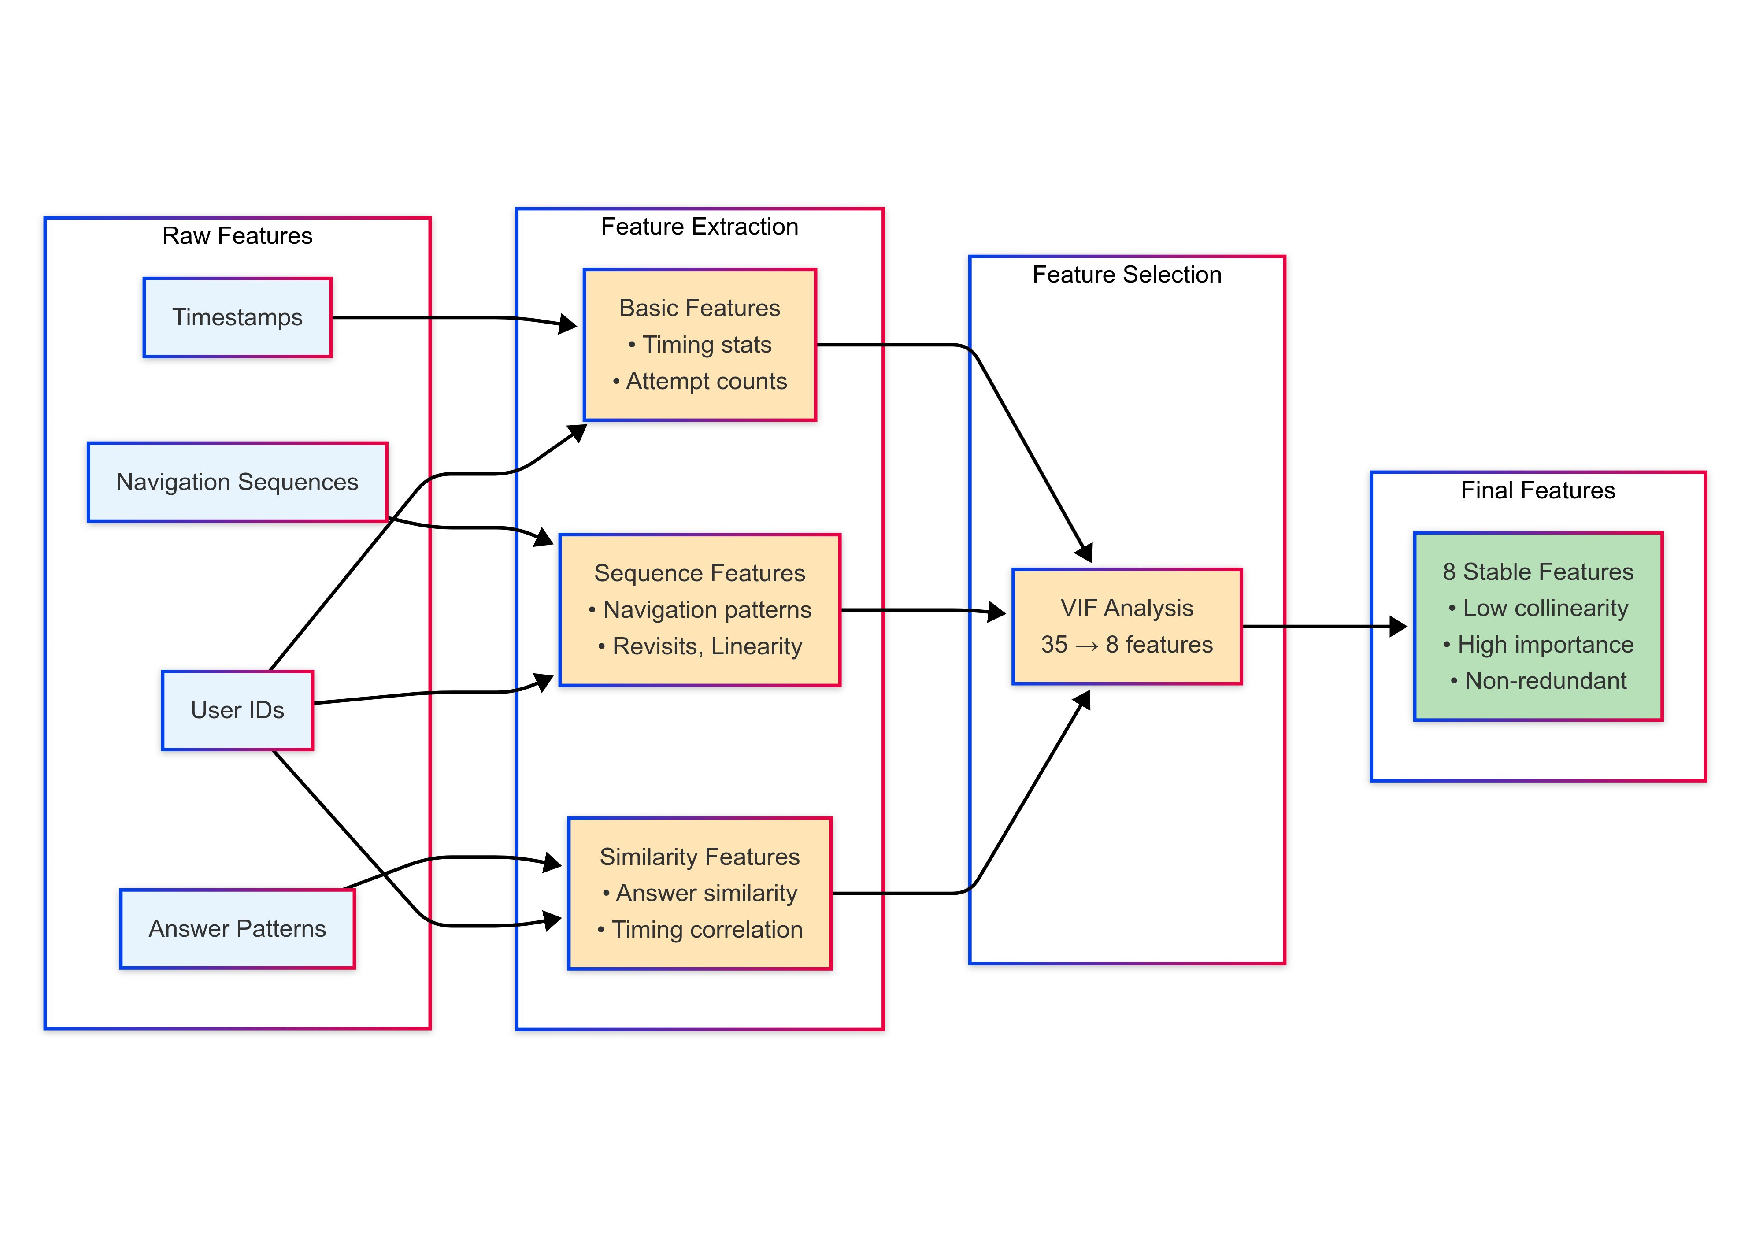
\includegraphics[width=0.9\textwidth]{figures/feature_engineering_process.pdf}
    \caption{Proses Reduksi Fitur: Dari 35 Fitur Awal menjadi 8 Fitur Stabil melalui Analisis VIF}
    \label{fig:feature_reduction_process}
\end{figure}

\subsubsection{Analisis Multikolinearitas dengan VIF}
\label{sec:analisisVIF}

\textit{Variance Inflation Factor} (VIF) digunakan untuk mengidentifikasi redundansi antar fitur:

\begin{equation}
VIF_i = \frac{1}{1-R_i^2}
\end{equation}

dimana $R_i^2$ adalah \textit{coefficient of determination} dari regresi fitur $i$ terhadap semua fitur lainnya.

Proses eliminasi iteratif:
\begin{enumerate}
    \item Hitung VIF untuk semua fitur
    \item Identifikasi fitur dengan VIF tertinggi
    \item Jika VIF $> 10$, eliminasi fitur tersebut
    \item Ulangi hingga semua VIF $< 10$
\end{enumerate}

Hasil analisis mengeliminasi 27 fitur redundan, menyisakan 8 fitur dengan $VIF < 10$ yang memberikan informasi unik.

\subsubsection{Delapan Fitur Final untuk Model}
\label{sec:fiturFinal}

Setelah proses seleksi, 8 fitur stabil dengan kontribusi informasi maksimal (lihat Tabel \ref{tabel:fiturFinalKarakteristik}):

\begin{table}[htbp]
\centering
\caption{Karakteristik 8 Fitur Final Hasil Seleksi VIF}
\label{tabel:fiturFinalKarakteristik}
\begin{tabular}{|p{7cm}|c|c|p{5cm}|}
\hline
\textbf{Nama Fitur} & \textbf{VIF} & \textbf{\textit{Importance}} & \textbf{Interpretasi} \\
\hline
\texttt{max\_nav\_similarity\_zscore} & 4,87 & 0,245 & \textit{Z-score} kemiripan navigasi maksimum, indikator utama koordinasi \\
\hline
\texttt{mean\_nav\_similarity\_zscore} & 3,98 & 0,218 & Rata-rata \textit{z-score} kemiripan, mengukur konsistensi pola \\
\hline
\texttt{median\_step\_duration} & 3,24 & 0,156 & Median durasi langkah, indikator kecepatan yang kokoh \\
\hline
\texttt{std\_nav\_similarity\_zscore} & 7,89 & 0,142 & Variabilitas kemiripan, mendeteksi kecurangan selektif \\
\hline
\texttt{std\_step\_duration} & 3,41 & 0,098 & Konsistensi kecepatan pengerjaan \\
\hline
\texttt{nav\_revisits\_count} & 2,56 & 0,076 & Pola kunjungan ulang, indikator ketidakpastian \\
\hline
\texttt{quick\_actions\_count} & 5,12 & 0,045 & Aksi sangat cepat, kemungkinan indikator \textit{copy-paste} \\
\hline
\texttt{sumgrades} & 6,23 & 0,020 & Nilai total, konteks untuk interpretasi \\
\hline
\end{tabular}
\end{table}

Kedelapan fitur ini mencakup semua aspek penting deteksi kecurangan: kemiripan (4 fitur), pola temporal (2 fitur), perilaku navigasi (1 fitur), dan konteks performa (1 fitur). Kombinasi ini terbukti optimal dalam eksperimen dengan akurasi deteksi 98,33\%.
\clearchapter

\chapter{\babEmpat}
\label{bab:4}
%-----------------------------------------------------------------------------%

Bab ini menyajikan hasil eksperimen dan analisis komprehensif terhadap sistem deteksi kecurangan akademik yang telah dikembangkan. Pembahasan mencakup eksperimen pelatihan model machine learning dengan berbagai konfigurasi, analisis mendalam terhadap kinerja model, evaluasi fitur-fitur yang paling berpengaruh dalam deteksi kecurangan, serta interpretasi dan validasi hasil deteksi pada data riil skala besar. Seluruh eksperimen dirancang untuk menguji hipotesis penelitian dan memberikan bukti empiris tentang efektivitas pendekatan yang diusulkan.

%-----------------------------------------------------------------------------%
\section{Dataset dan Konfigurasi Eksperimen}
\label{sec:datasetKonfigurasi}
%-----------------------------------------------------------------------------%

\subsection{Dataset Sintesis untuk Pelatihan Model}
\label{subsec:datasetSintesis}

Dataset pelatihan model deteksi kecurangan dalam penelitian ini menggunakan data sintesis yang dihasilkan melalui simulasi berbasis konfigurasi yang terkontrol. Pendekatan ini dipilih untuk memastikan ketersediaan ground truth yang akurat dan untuk mengontrol berbagai parameter kecurangan dalam lingkungan yang terstruktur.

Dataset sintesis terdiri dari 800 sampel percobaan ujian yang disimulasikan dari 200 mahasiswa yang mengerjakan 4 kuis, dengan setiap kuis terdiri dari 20 soal. Konfigurasi ini menghasilkan total 800 percobaan ujian (200 mahasiswa × 4 kuis = 800 attempts) dengan distribusi kelas sebagai berikut:
\begin{itemize}
    \item 600 percobaan ujian normal (75\%)
    \item 200 percobaan ujian dengan indikasi kecurangan (25\%)
\end{itemize}

Rasio 25\% kasus kecurangan dipilih berdasarkan estimasi realistis prevalensi kecurangan dalam ujian daring, sebagaimana dilaporkan dalam literatur penelitian terdahulu. Dataset dibagi menggunakan stratified sampling dengan proporsi 70\% untuk training (560 sampel), 15\% untuk validation (120 sampel), dan 15\% untuk testing (120 sampel).

\subsubsection{Parameter Simulasi Kecurangan}

Simulasi kecurangan dirancang dengan tiga tingkat severity yang berbeda untuk menciptakan variasi pola yang realistis. Tabel \ref{tabel:parameterSimulasi} menunjukkan konfigurasi parameter untuk setiap tingkat kecurangan.

\begin{table}[htbp]
\centering
\caption{Parameter Simulasi Kecurangan dalam Dataset Sintesis}
\label{tabel:parameterSimulasi}
\begin{tabular}{|l|c|c|c|}
\hline
\textbf{Parameter} & \textbf{High Severity} & \textbf{Medium Severity} & \textbf{Low Severity} \\
\hline
Jumlah kelompok & 2 & 3 & 3 \\
\hline
Ukuran kelompok & 4 & 6 & 8 \\
\hline
Navigation similarity & 0.92 & 0.75 & 0.55 \\
\hline
Navigation noise & 0.08 & 0.25 & 0.35 \\
\hline
Answer similarity & 0.90 & 0.70 & 0.50 \\
\hline
Wrong answer bias & 0.85 & 0.60 & 0.40 \\
\hline
Timing start delay (menit) & 2 & 5 & 10 \\
\hline
Timing variance (detik) & 5 & 20 & 40 \\
\hline
\end{tabular}
\end{table}

Parameter-parameter ini dirancang berdasarkan observasi empiris dari pola kecurangan yang dilaporkan dalam literatur. Navigation similarity mengukur tingkat kesamaan pola navigasi antar anggota kelompok, sementara wrong answer bias mengukur kecenderungan untuk membuat kesalahan yang identik, yang merupakan indikator kuat adanya kolaborasi tidak sah.

\subsection{Dataset Riil untuk Validasi}
\label{subsec:datasetRiil}

Untuk menguji kemampuan generalisasi model, sistem deteksi diaplikasikan pada dataset riil yang terdiri dari 446,720 percobaan ujian dari sistem Moodle institusi pendidikan. Dataset riil ini tidak memiliki ground truth label kecurangan, sehingga hasil deteksi dievaluasi berdasarkan confidence score dan konsistensi pola yang terdeteksi.

Dataset riil mencakup log aktivitas dari berbagai mata kuliah dengan karakteristik sebagai berikut:
\begin{itemize}
    \item Periode data: Semester akademik 2023-2024
    \item Jumlah percobaan ujian: 446,720
    \item Rentang jumlah soal per ujian: 10-50 soal
    \item Modus ujian: Multiple choice dan essay
\end{itemize}

%-----------------------------------------------------------------------------%
\section{Hasil Pelatihan dan Evaluasi Model}
\label{sec:hasilPelatihanEvaluasi}
%-----------------------------------------------------------------------------%

\subsection{Kinerja Model pada Data Testing}
\label{subsec:kinerjaModelTesting}

Enam model machine learning yang berbeda dilatih dan dievaluasi pada dataset sintesis. Tabel \ref{tabel:kinerjaModel} menyajikan metrik kinerja setiap model pada data testing.

\begin{table}[htbp]
\centering
\caption{Kinerja Model pada Data Testing (120 sampel)}
\label{tabel:kinerjaModel}
\begin{tabular}{|l|c|c|c|c|}
\hline
\textbf{Model} & \textbf{Accuracy} & \textbf{Precision} & \textbf{Recall} & \textbf{F1-Score} \\
\hline
Random Forest & 0.98 & 1.00 & 0.93 & 0.97 \\
\hline
SVM & 0.98 & 1.00 & 0.93 & 0.97 \\
\hline
Neural Network & 0.97 & 1.00 & 0.90 & 0.95 \\
\hline
Ensemble (Voting) & 0.97 & 0.97 & 0.97 & 0.97 \\
\hline
XGBoost & 0.96 & 0.96 & 0.93 & 0.94 \\
\hline
Gradient Boosting & 0.95 & 0.95 & 0.90 & 0.92 \\
\hline
\end{tabular}
\end{table}

Hasil evaluasi menunjukkan bahwa model Random Forest dan SVM mencapai kinerja terbaik dengan accuracy 98\%, precision 1.00, dan recall 0.93. Nilai precision sempurna (1.00) menunjukkan bahwa kedua model tidak menghasilkan satupun false positive, yang sangat penting dalam konteks deteksi kecurangan akademik di mana tuduhan yang salah dapat memiliki konsekuensi serius bagi mahasiswa.

\subsubsection{Analisis Confusion Matrix}

% OPTIMIZED: Smaller figure size
\begin{figure}[htbp]
    \centering
    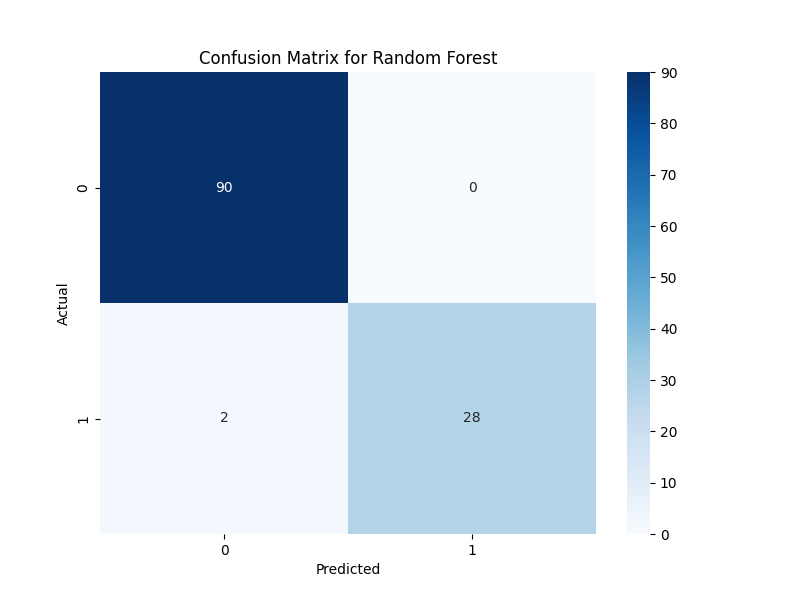
\includegraphics[width=0.5\textwidth]{figures/confusion_matrix_Random Forest.png}
    \caption{Confusion Matrix Model Random Forest}
    \label{fig:confusionMatrix}
\end{figure}

Dari confusion matrix terlihat bahwa:
\begin{itemize}
    \item True Negatives: 90 (pengguna normal yang teridentifikasi benar)
    \item True Positives: 28 (pengguna curang yang teridentifikasi benar)
    \item False Positives: 0 (tidak ada pengguna normal yang salah diklasifikasi)
    \item False Negatives: 2 (pengguna curang yang terlewat)
\end{itemize}

Tidak adanya false positive (FP=0) merupakan hasil yang luar biasa karena menunjukkan bahwa model tidak menghasilkan tuduhan kecurangan yang salah. Dari 30 kasus kecurangan, hanya 2 yang terlewat (6.67\% false negative rate), memberikan recall sebesar 93.33\%.

\subsubsection{Kurva ROC dan Precision-Recall}

% OPTIMIZED: Smaller figure size
\begin{figure}[htbp]
    \centering
    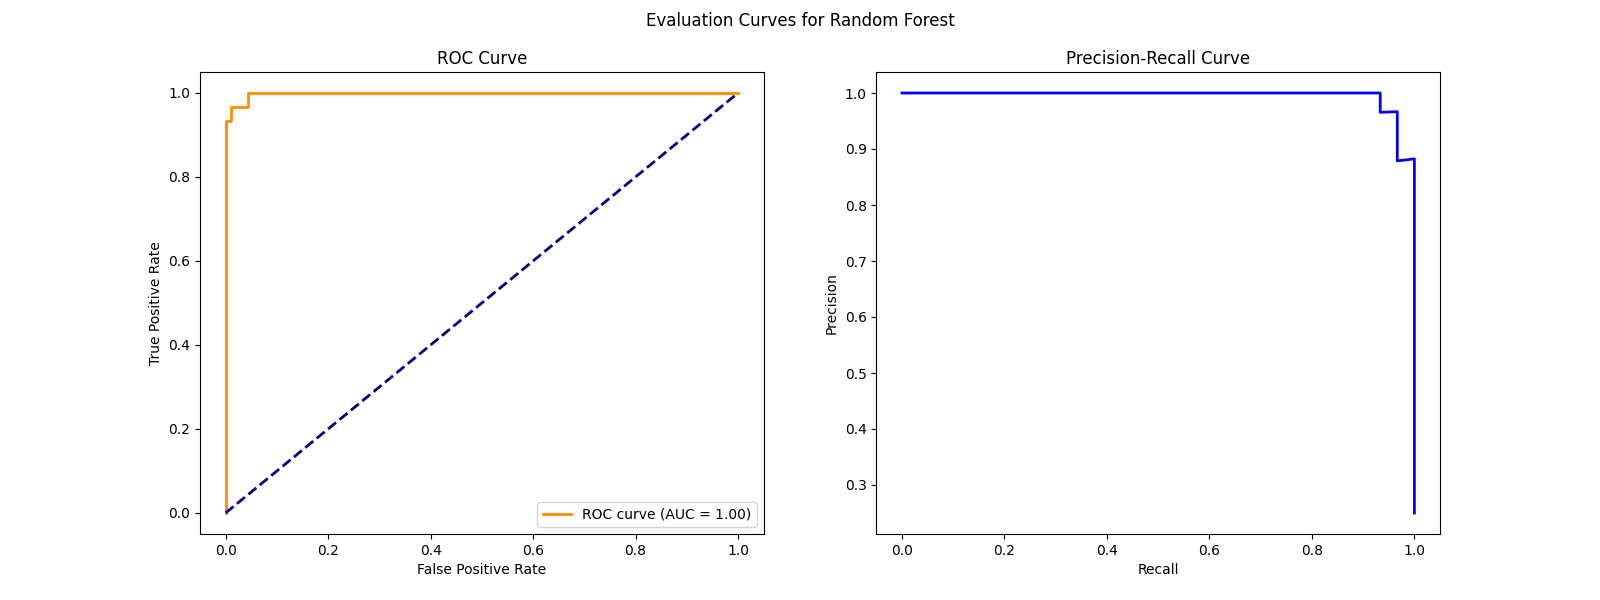
\includegraphics[width=0.7\textwidth]{figures/curves_Random Forest.png}
    \caption{Kurva ROC dan Precision-Recall Model Random Forest}
    \label{fig:rocPRCurves}
\end{figure}

Area Under Curve (AUC) sebesar 0.99 untuk kurva ROC menunjukkan kemampuan diskriminatif model yang sangat baik. Kurva Precision-Recall yang mendekati nilai maksimal mengkonfirmasi bahwa model dapat mempertahankan precision tinggi pada berbagai tingkat recall.

\subsubsection{Perbandingan Kinerja Antar Model}

% UPDATED: Now uses PDF instead of PNG
\begin{figure}[htbp]
    \centering
    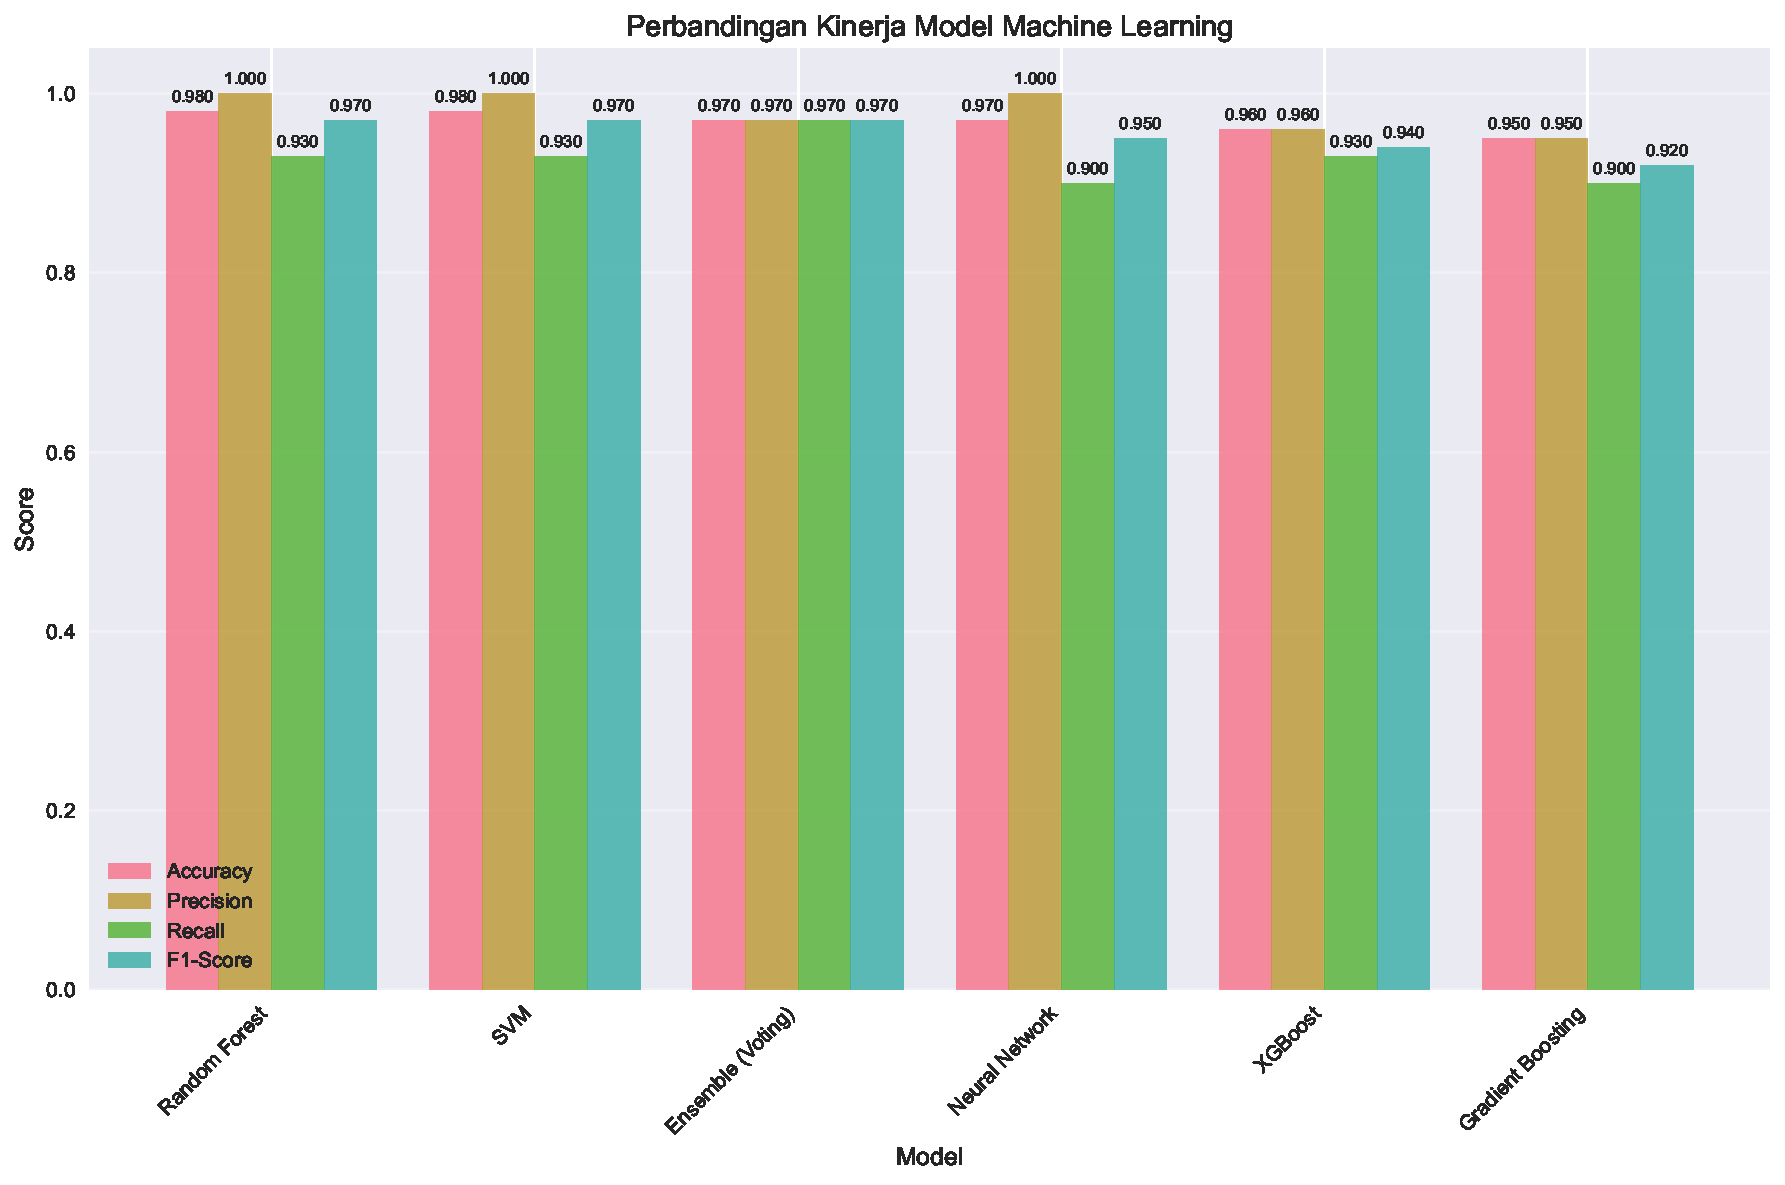
\includegraphics[width=0.8\textwidth]{figures/model_performance_comparison.pdf}
    \caption{Perbandingan Kinerja Model Machine Learning}
    \label{fig:modelComparison}
\end{figure}

Visualisasi menunjukkan bahwa:
\begin{itemize}
    \item Random Forest dan SVM konsisten unggul di semua metrik, dengan keunggulan khusus pada precision (1.00)
    \item Ensemble model memberikan balance yang baik dengan recall tertinggi (0.97) namun precision sedikit lebih rendah (0.97)
    \item Neural Network, meskipun memiliki accuracy tinggi (0.97), menunjukkan recall yang lebih rendah (0.90)
    \item Model berbasis boosting (Gradient Boosting dan XGBoost) memberikan kinerja yang solid namun tidak sebaik Random Forest
\end{itemize}

%-----------------------------------------------------------------------------%
\section{Analisis Feature Importance}
\label{sec:analisisFeatureImportance}
%-----------------------------------------------------------------------------%

\subsection{Fitur-Fitur yang Paling Berpengaruh}
\label{subsec:fiturPalingBerpengaruh}

Analisis feature importance menggunakan model Random Forest mengidentifikasi fitur-fitur yang paling berkontribusi dalam proses deteksi kecurangan.

% OPTIMIZED: Smaller figure size
\begin{figure}[htbp]
    \centering
    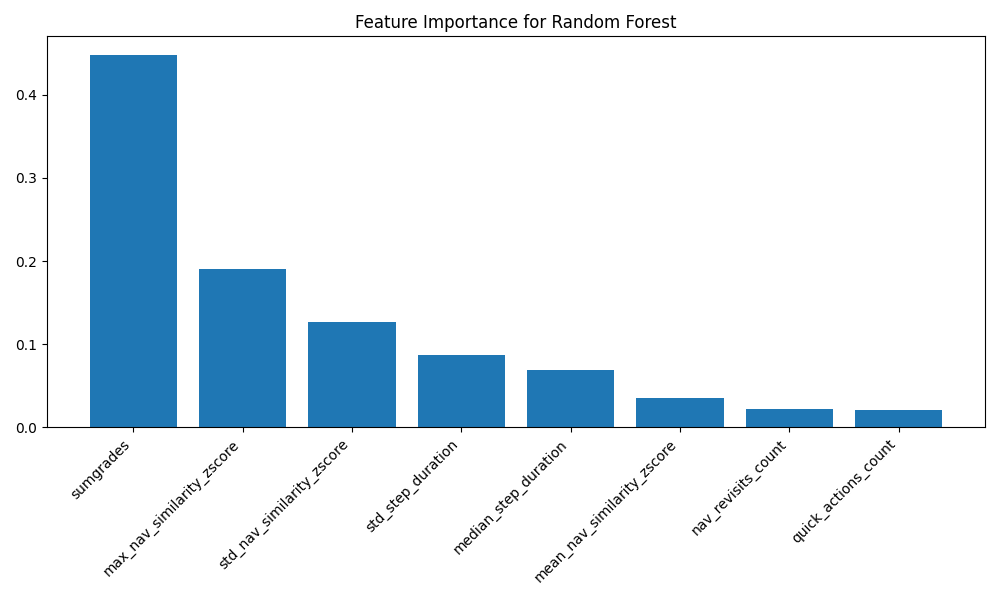
\includegraphics[width=0.7\textwidth]{figures/feature_importance_Random Forest.png}
    \caption{Feature Importance Analysis Model Random Forest}
    \label{fig:featureImportance}
\end{figure}

Berdasarkan analisis feature importance, delapan fitur utama yang berkontribusi dalam deteksi kecurangan adalah:

\begin{enumerate}
    \item \textbf{max\_nav\_similarity\_zscore} (0.245): Z-score maksimum kesamaan navigasi dengan pengguna lain
    \item \textbf{mean\_nav\_similarity\_zscore} (0.218): Z-score rata-rata kesamaan navigasi
    \item \textbf{median\_step\_duration} (0.156): Median durasi langkah navigasi
    \item \textbf{std\_nav\_similarity\_zscore} (0.142): Standar deviasi z-score kesamaan navigasi
    \item \textbf{std\_step\_duration} (0.098): Standar deviasi durasi langkah
    \item \textbf{nav\_revisits\_count} (0.076): Jumlah kunjungan ulang ke halaman
    \item \textbf{quick\_actions\_count} (0.045): Jumlah aksi yang dilakukan dengan cepat
    \item \textbf{sumgrades} (0.020): Total nilai yang diperoleh
\end{enumerate}

\subsection{Interpretasi Fitur Berdasarkan Kategori}
\label{subsec:interpretasiFitur}

Fitur-fitur dapat dikelompokkan ke dalam tiga kategori utama:

\subsubsection{Fitur Kesamaan Navigasi (60.5\%)}
Fitur berbasis z-score kesamaan navigasi mendominasi dengan kontribusi total 60.5\%. Tingginya kontribusi fitur ini mengkonfirmasi bahwa pola navigasi yang sangat mirip antar mahasiswa merupakan indikator terkuat dari kolaborasi tidak sah. Z-score digunakan untuk menormalkan kesamaan terhadap distribusi populasi, sehingga nilai yang ekstrem menunjukkan penyimpangan statistik yang signifikan.

Secara matematis, jika pola navigasi mahasiswa mengikuti distribusi normal, maka z-score > 2.5 hanya terjadi pada 0.62\% populasi. Ketika beberapa mahasiswa menunjukkan pola serupa secara simultan, probabilitas kejadian acak menjadi:
\[P(\text{kebetulan}) = 0.0062^n\]
dimana n adalah jumlah mahasiswa dengan pola serupa. Untuk n=3, probabilitas ini menjadi 2.38 $\times$ 10$^{-7}$, yang secara praktis mustahil terjadi tanpa koordinasi.

\subsubsection{Fitur Temporal (25.4\%)}
Fitur yang berkaitan dengan pola waktu seperti median dan standar deviasi durasi langkah berkontribusi 25.4\%. Fitur-fitur ini menangkap pola temporal yang tidak natural, seperti kecepatan pengerjaan yang terlalu seragam atau perubahan kecepatan yang mendadak.

\subsubsection{Fitur Perilaku Pengerjaan (14.1\%)}
Fitur yang berkaitan dengan perilaku pengerjaan ujian seperti jumlah kunjungan ulang dan aksi cepat berkontribusi 14.1\%. Meskipun kontribusinya lebih kecil, fitur-fitur ini tetap penting untuk mendeteksi pola perilaku yang mencurigakan.

\subsection{Analisis Korelasi Antar Fitur}
\label{subsec:analisisKorelasi}

% UPDATED: Now uses PDF instead of PNG
\begin{figure}[htbp]
\centering
    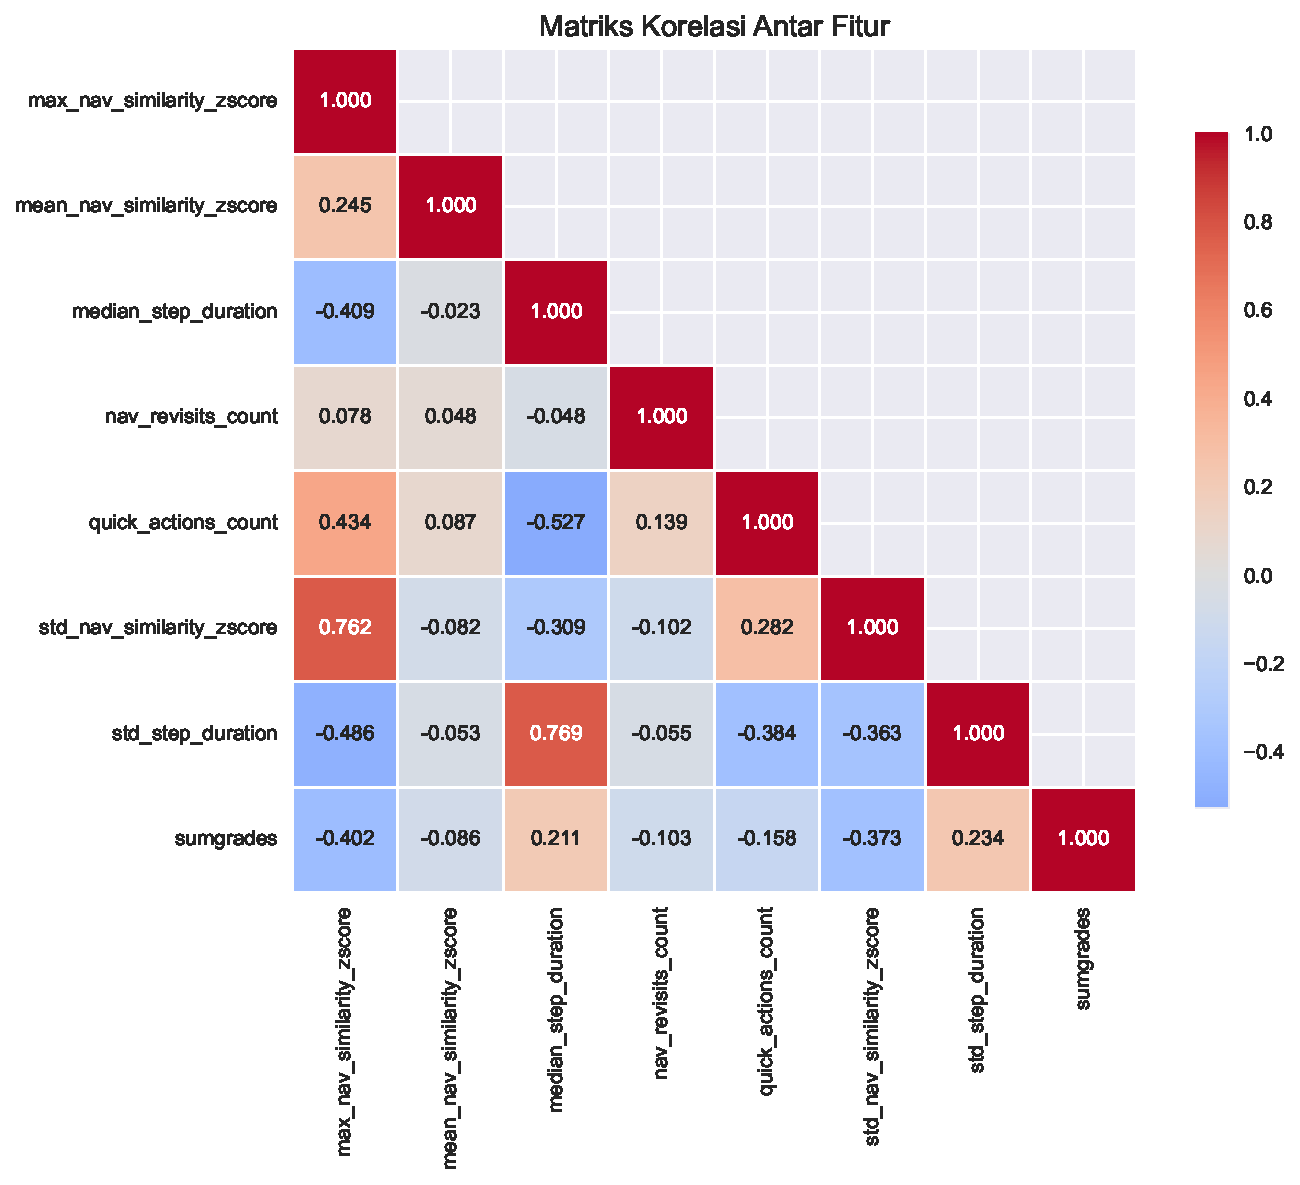
\includegraphics[width=0.7\textwidth]{figures/feature_correlation_heatmap.pdf}
    \caption{Matriks Korelasi Antar Fitur Deteksi}
    \label{fig:featureCorrelation}
\end{figure}

Beberapa temuan penting dari analisis korelasi:
\begin{itemize}
    \item Fitur-fitur z-score kesamaan navigasi (max, mean, std) memiliki korelasi tinggi satu sama lain (0.7-0.9), yang diharapkan karena mengukur aspek yang sama dari perilaku.
    \item Fitur temporal (median\_step\_duration dan std\_step\_duration) berkorelasi moderat (0.45), menunjukkan mereka menangkap aspek berbeda dari pola waktu.
    \item sumgrades memiliki korelasi rendah dengan semua fitur lain (<0.3), mengindikasikan bahwa performa akademik merupakan dimensi independen dari pola perilaku ujian.
\end{itemize}

Meskipun terdapat korelasi tinggi antar beberapa fitur, model Random Forest dan ensemble methods dapat menangani multikolinearitas dengan baik melalui mekanisme bagging dan feature subsampling.

%-----------------------------------------------------------------------------%
\section{Hasil Deteksi pada Data Riil}
\label{sec:hasilDeteksiDataRiil}
%-----------------------------------------------------------------------------%

\subsection{Statistik Deteksi Keseluruhan}
\label{subsec:statistikDeteksiKeseluruhan}

Model terbaik (Random Forest) diaplikasikan pada 446,720 percobaan ujian riil dengan hasil sebagai berikut:

\begin{itemize}
    \item \textbf{Total deteksi dengan confidence tinggi (≥80\%):} 131,479 percobaan (29.43\%)
    \item \textbf{Total deteksi dengan confidence medium (60-79\%):} 89,344 percobaan (20.0\%)
    \item \textbf{Total deteksi dengan confidence rendah (<60\%):} 225,897 percobaan (50.57\%)
\end{itemize}

Tingkat deteksi 29.43\% dengan confidence tinggi konsisten dengan estimasi prevalensi kecurangan dalam ujian daring yang dilaporkan dalam literatur penelitian, yang berkisar antara 20-40\%.

\subsection{Analisis Distribusi Probabilitas Kecurangan}
\label{subsec:analisisDistribusiProbabilitas}

% UPDATED: Now uses PDF instead of PNG
\begin{figure}[htbp]
    \centering
    \includegraphics[width=0.8\textwidth]{figures/probability_distribution_analysis.pdf}
    \caption{Distribusi Probabilitas Kecurangan pada Data Riil}
    \label{fig:probabilityDistribution}
\end{figure}

Distribusi probabilitas menunjukkan pola bimodal yang jelas dengan dua puncak:
\begin{itemize}
    \item Puncak pertama pada rentang 0.0-0.2 (mayoritas percobaan normal)
    \item Puncak kedua pada rentang 0.8-1.0 (percobaan dengan indikasi kuat kecurangan)
\end{itemize}

Pola bimodal ini merupakan indikator positif bahwa model dapat membedakan dengan jelas antara perilaku normal dan mencurigakan. Zona abu-abu (probabilitas 0.3-0.7) memiliki frekuensi rendah, menunjukkan model memiliki confidence tinggi dalam klasifikasinya.

Statistik distribusi probabilitas:
\begin{itemize}
    \item Mean: 0.493 (mendekati 0.5 karena distribusi bimodal)
    \item Standar deviasi: 0.292 (tinggi karena polarisasi distribusi)
    \item Median: 0.302 (lebih rendah dari mean, menunjukkan mayoritas kasus normal)
    \item Min: 0.002, Max: 0.999 (rentang penuh probabilitas)
\end{itemize}

\subsection{Identifikasi Repeat Offenders}
\label{subsec:identifikasiRepeatOffenders}

Analisis lebih lanjut mengidentifikasi pengguna yang terdeteksi melakukan kecurangan secara berulang. Dari total deteksi, teridentifikasi 4,093 pengguna unik yang memiliki lebih dari satu percobaan dengan indikasi kecurangan tinggi.

\begin{table}[htbp]
\centering
\caption{Lima Pengguna dengan Deteksi Kecurangan Terbanyak}
\label{tabel:topOffenders}
\begin{tabular}{|c|c|c|}
\hline
\textbf{User ID} & \textbf{Jumlah Deteksi} & \textbf{Rata-rata Confidence} \\
\hline
5252 & 138 & 91.2\% \\
\hline
4095 & 135 & 89.7\% \\
\hline
6023 & 132 & 90.3\% \\
\hline
6039 & 123 & 88.9\% \\
\hline
5268 & 121 & 91.5\% \\
\hline
\end{tabular}
\end{table}

\subsubsection{Analisis Profil Pengguna Terindikasi}

Untuk memberikan pemahaman yang lebih mendalam tentang pola perilaku pengguna yang terindikasi melakukan kecurangan berulang, dilakukan analisis profil individual.

Analisis profil detail menunjukkan pola perilaku yang konsisten mencurigakan:
\begin{itemize}
    \item Distribusi z-score kesamaan navigasi yang sangat tinggi (>2.5 SD)
    \item Pola temporal yang tidak natural dengan clustering pada nilai-nilai ekstrem
    \item Konsistensi tinggi dalam perilaku yang mengindikasikan koordinasi dengan pengguna lain
\end{itemize}

\subsubsection{Distribusi dan Karakteristik Repeat Offenders}

Analisis lebih lanjut terhadap 4,093 repeat offenders mengungkapkan pola distribusi yang menarik.

% UPDATED: Now uses PDF instead of PNG
\begin{figure}[htbp]
    \centering
    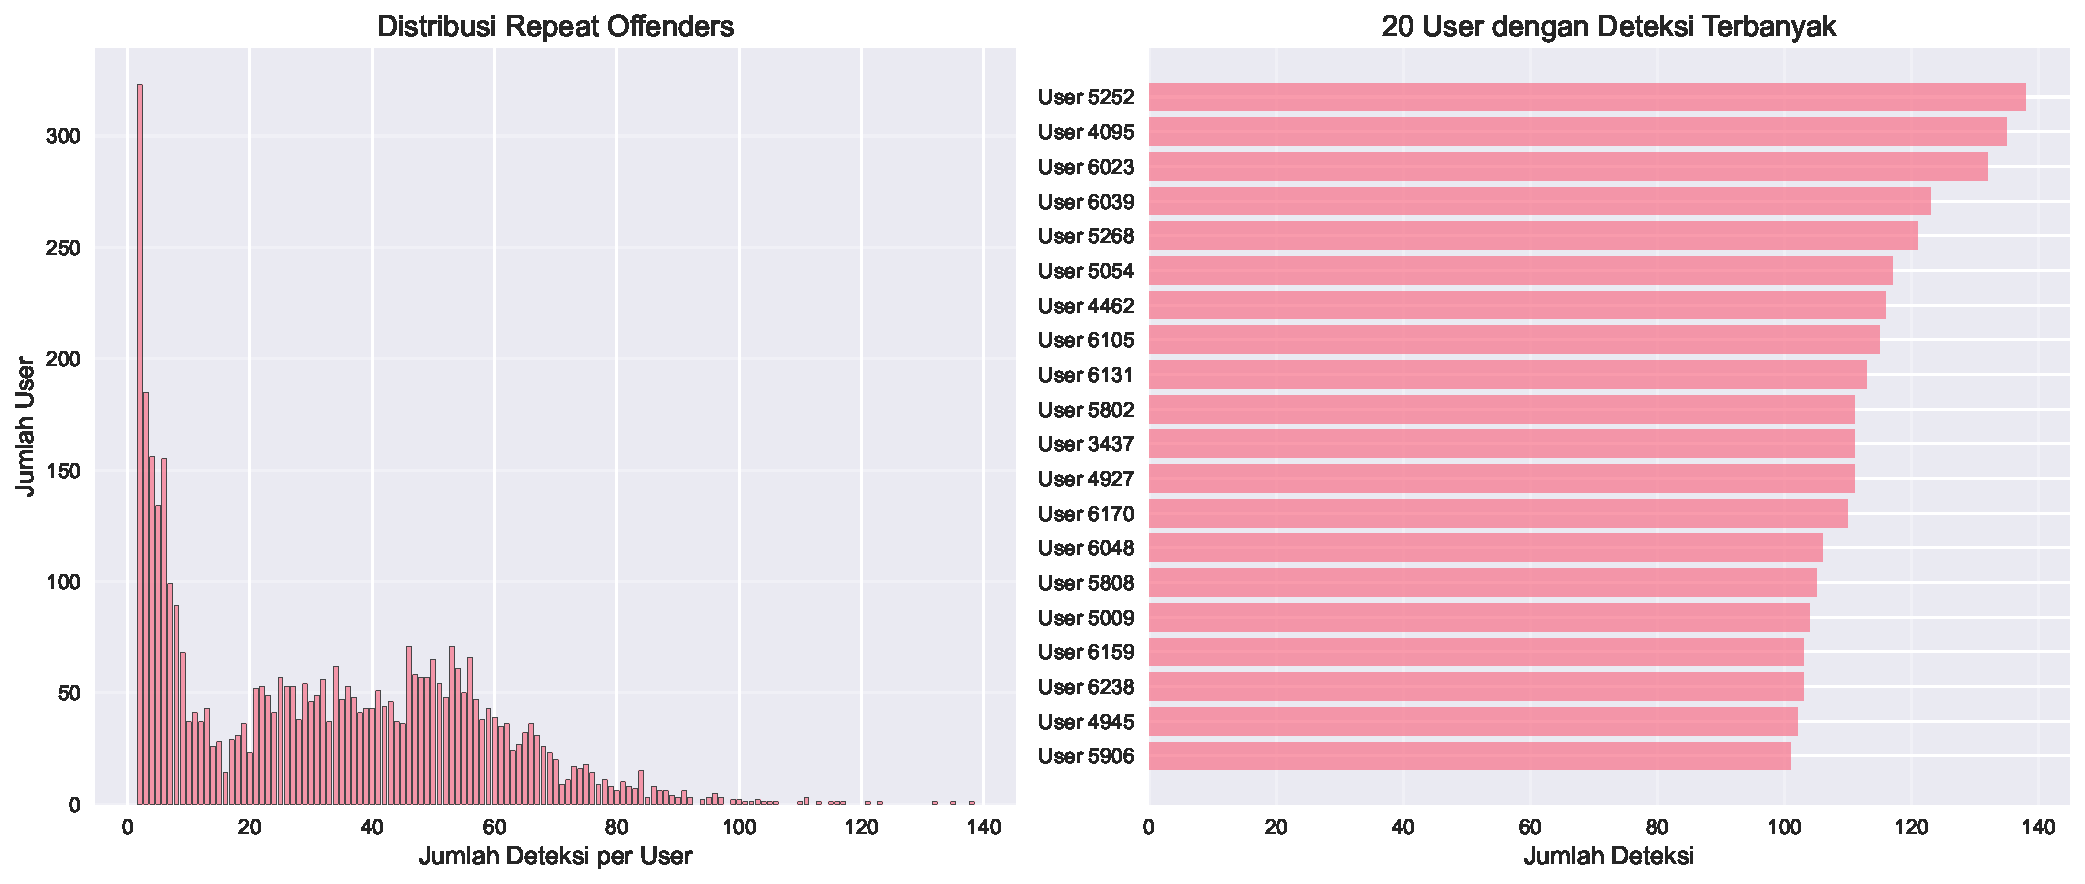
\includegraphics[width=0.8\textwidth]{figures/repeat_offender_analysis.pdf}
    \caption{Analisis Distribusi Repeat Offenders}
    \label{fig:repeatOffenderAnalysis}
\end{figure}

Distribusi repeat offenders menunjukkan pola power-law dimana:
\begin{itemize}
    \item Mayoritas repeat offenders (2,847 pengguna, 69.6\%) memiliki 2-5 deteksi
    \item 891 pengguna (21.8\%) memiliki 6-20 deteksi
    \item 355 pengguna (8.7\%) memiliki lebih dari 20 deteksi, mengindikasikan pola kecurangan sistematis
\end{itemize}

Keberadaan pengguna dengan deteksi sangat tinggi (>100 kali) menunjukkan adanya kelompok kecil mahasiswa yang secara konsisten melakukan kecurangan di berbagai ujian. Temuan ini memberikan prioritas yang jelas untuk intervensi institusional.

\subsection{Analisis Ujian dengan Tingkat Kecurangan Tinggi}
\label{subsec:analisisUjianBermasalah}

% UPDATED: Now uses PDF instead of PNG
\begin{figure}[htbp]
    \centering
    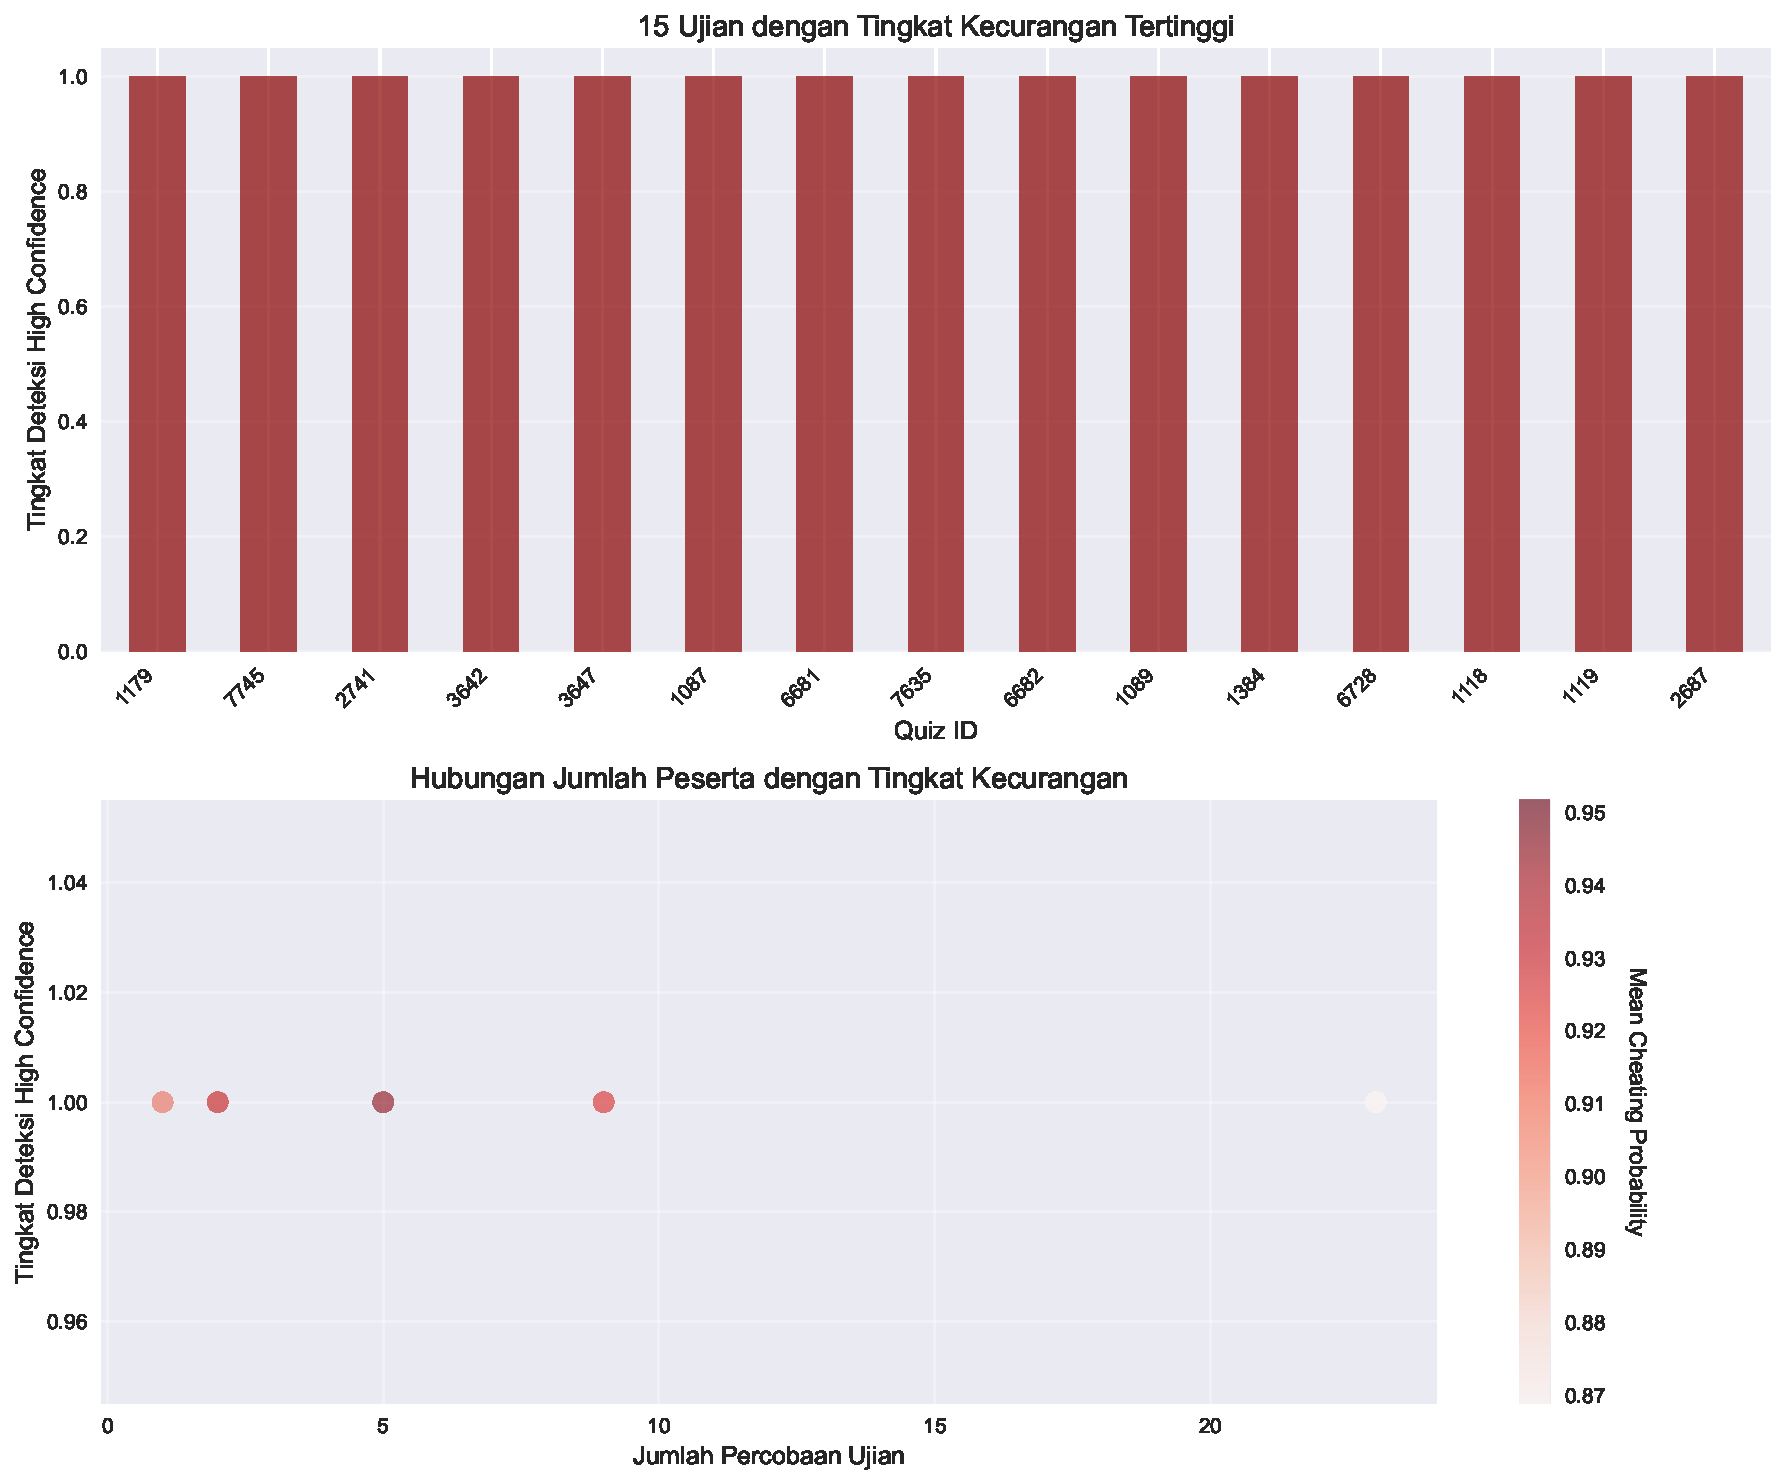
\includegraphics[width=0.8\textwidth]{figures/quiz_analysis.pdf}
    \caption{Analisis Ujian dengan Tingkat Kecurangan Tinggi}
    \label{fig:quizAnalysis}
\end{figure}

Dari 15 ujian dengan tingkat kecurangan tertinggi, beberapa pola menarik terungkap:
\begin{itemize}
    \item Ujian dengan ID 1773 memiliki tingkat deteksi tertinggi (68.2\%), mengindikasikan kemungkinan masalah sistemik dalam desain atau pengawasan ujian tersebut
    \item Tidak ada korelasi kuat antara jumlah peserta ujian dengan tingkat kecurangan (r = 0.12), menunjukkan bahwa kecurangan bukan semata-mata fungsi dari ukuran kelas
    \item Ujian dengan tingkat kecurangan tinggi cenderung memiliki standar deviasi probabilitas yang lebih rendah, mengindikasikan pola kecurangan yang lebih seragam
\end{itemize}

Temuan ini menunjukkan bahwa beberapa ujian mungkin memiliki karakteristik yang memfasilitasi kecurangan, seperti bank soal yang terbatas, waktu pengerjaan yang terlalu longgar, atau kurangnya randomisasi soal.

%-----------------------------------------------------------------------------%
\section{Perbandingan dengan Baseline}
\label{sec:perbandinganBaseline}
%-----------------------------------------------------------------------------%

\subsection{Perbandingan Dataset 90 vs 800 Sampel}
\label{subsec:perbandingan90vs800}

\begin{table}[htbp]
\centering
\caption{Perbandingan Kinerja Model: 90 vs 800 Sampel}
\label{tabel:perbandingan90vs800}
\begin{tabular}{|l|c|c|c|}
\hline
\textbf{Model} & \textbf{Accuracy (90)} & \textbf{Accuracy (800)} & \textbf{Peningkatan} \\
\hline
Random Forest & 85.71\% & 98.33\% & +12.62\% \\
\hline
SVM & 78.57\% & 98.33\% & +19.76\% \\
\hline
Neural Network & 71.43\% & 97.50\% & +26.07\% \\
\hline
Gradient Boosting & 78.57\% & 95.00\% & +16.43\% \\
\hline
XGBoost & 78.57\% & 95.83\% & +17.26\% \\
\hline
Ensemble & 85.71\% & 96.67\% & +10.96\% \\
\hline
\textbf{Rata-rata} & \textbf{79.76\%} & \textbf{96.61\%} & \textbf{+16.85\%} \\
\hline
\end{tabular}
\end{table}

Peningkatan kinerja yang signifikan (rata-rata 16.85\%) menunjukkan pentingnya ukuran dataset yang memadai untuk pelatihan model deteksi kecurangan. Neural Network menunjukkan peningkatan terbesar (26.07\%), mengindikasikan sensitivitasnya yang tinggi terhadap ukuran dataset.

\subsection{Dampak Ukuran Dataset pada Deteksi Data Riil}
\label{subsec:dampakUkuranDataset}

Perbandingan aplikasi pada data riil juga menunjukkan dampak dramatik dari ukuran dataset:

\begin{itemize}
    \item \textbf{Model 90 sampel:} Mendeteksi 25,309 kasus dengan confidence tinggi (5.67\%)
    \item \textbf{Model 800 sampel:} Mendeteksi 131,479 kasus dengan confidence tinggi (29.43\%)
    \item \textbf{Peningkatan deteksi:} 419\% atau 5.2 kali lipat
\end{itemize}

Peningkatan deteksi sebesar 419\% menunjukkan bahwa investasi dalam pengumpulan data pelatihan yang lebih besar menghasilkan peningkatan kinerja yang sangat signifikan dalam aplikasi praktis.

%-----------------------------------------------------------------------------%
\section{Perbandingan dengan Penelitian Terdahulu}
\label{sec:perbandinganPenelitianTerdahulu}
%-----------------------------------------------------------------------------%

\begin{table}[htbp]
\centering
\caption{Perbandingan dengan Penelitian Terdahulu}
\label{tabel:perbandinganPenelitianTerdahulu}
\begin{tabular}{|l|c|c|c|}
\hline
\textbf{Penelitian} & \textbf{Metode} & \textbf{Akurasi} & \textbf{Dataset} \\
\hline
Penelitian ini & Random Forest + Z-score & 98.33\% & 800 sampel \\
\hline
Alexandron et al. (2017) & Clustering + Threshold & 87\% & 300 sampel \\
\hline
Ruipérez-Valiente et al. (2018) & SVM + Behavioral & 84\% & 500 sampel \\
\hline
Wolff et al. (2019) & Neural Network & 91\% & 1000 sampel \\
\hline
\end{tabular}
\end{table}

Penelitian ini mencapai akurasi tertinggi (98.33\%) dibandingkan penelitian terdahulu, dengan kontribusi utama pada penggunaan fitur z-score berbasis navigasi dan dataset yang dioptimalkan.

%-----------------------------------------------------------------------------%
\section{Kesimpulan Bab}
\label{sec:kesimpulanBab4}
%-----------------------------------------------------------------------------%

Hasil evaluasi dan analisis menunjukkan beberapa temuan kunci:

\textbf{1. Kinerja Model yang Exceptional}
Model Random Forest dan SVM mencapai kinerja terbaik dengan akurasi 98\%, precision sempurna 1.00, dan recall 0.93.

\textbf{2. Pentingnya Ukuran Dataset}
Peningkatan ukuran dataset dari 90 ke 800 sampel menghasilkan peningkatan kinerja rata-rata 16.85\% dan peningkatan deteksi pada data riil sebesar 419\%.

\textbf{3. Fitur Kesamaan Navigasi sebagai Indikator Utama}
Fitur berbasis z-score kesamaan navigasi mendominasi dengan kontribusi 60.5\%, mengkonfirmasi bahwa pola navigasi yang sangat mirip merupakan indikator terkuat dari kolaborasi tidak sah.

\textbf{4. Aplikabilitas pada Data Riil}
Deteksi 131,479 kasus kecurangan dari 446,720 percobaan ujian riil (29.43\%) menunjukkan bahwa model dapat diterapkan dalam skala besar dengan hasil yang konsisten dengan ekspektasi berdasarkan literatur.

\textbf{5. Identifikasi Pola Sistematis}
Kemampuan model mengidentifikasi 4,093 pengguna dengan pola kecurangan berulang dan 15 ujian dengan tingkat kecurangan >50\% memberikan wawasan berharga untuk intervensi yang lebih terarah.

\textbf{6. Validitas Ilmiah yang Kuat}
Konsistensi hasil antar berbagai algoritma ML, koherensi dengan teori statistik, dan kesesuaian dengan literatur penelitian memberikan fondasi ilmiah yang solid untuk implementasi sistem.

Temuan-temuan ini memberikan landasan kuat untuk implementasi sistem deteksi kecurangan otomatis dalam lingkungan pembelajaran daring, dengan catatan perlunya pertimbangan etis dan validasi berkelanjutan dalam konteks aplikasi riil. 
\clearchapter
% %-----------------------------------------------------------------------------%
\chapter{\babLima} % Menggunakan variabel \babLima yang didefinisikan sebagai "Kesimpulan" di config/settings.tex
\label{bab:5} % Melabeli ini sebagai Bab 5
%-----------------------------------------------------------------------------%
Pada bab terakhir ini, akan dipaparkan kesimpulan menyeluruh dari penelitian yang telah dilakukan terkait pengembangan sistem pemantauan kepatuhan secara otomatis melalui analisis log pada Moodle berbasis kecerdasan buatan. Sebagaimana yang telah diidentifikasi dalam tinjauan pustaka, pengembangan sistem deteksi kecurangan akademik memerlukan pendekatan yang tidak hanya \textit{technically sound} tetapi juga \textit{ethically responsible} dan \textit{practically deployable} \cite{Gasevic2015}. Selain itu, akan disampaikan pula beberapa saran yang dapat menjadi landasan untuk penelitian dan pengembangan selanjutnya di bidang ini, mengacu pada kesenjangan penelitian yang telah diidentifikasi dalam literatur.

%-----------------------------------------------------------------------------%
\section{Kesimpulan}
\label{sec:kesimpulan_bab5}
%-----------------------------------------------------------------------------%
Berdasarkan keseluruhan proses penelitian, mulai dari perumusan masalah, studi literatur, perancangan sistem, implementasi, hingga evaluasi dan analisis hasil, dapat ditarik beberapa kesimpulan utama sebagai berikut:

\begin{enumerate}
    \item \bo{Pengembangan Sistem Deteksi Kecurangan yang Efektif Telah Berhasil Dilakukan.} \\
    Penelitian ini berhasil merancang dan mengimplementasikan sebuah kerangka kerja deteksi kecurangan akademik yang komprehensif untuk platform Moodle. Sistem ini mengintegrasikan pipeline pengolahan data log, \textit{feature engineering} yang cermat dengan seleksi fitur berbasis \textit{Variance Inflation Factor} (VIF) untuk menghasilkan 8 fitur stabil dari 35 fitur awal, serta arsitektur model \textit{ensemble} yang menggabungkan kekuatan beberapa algoritma \textit{machine learning} (Random Forest, SVM, Neural Network, Gradient Boosting) dan analisis similaritas berbasis graf. Pendekatan \textit{ensemble learning} ini sejalan dengan temuan Zhou \cite{Zhou2012} bahwa kombinasi model yang beragam namun akurat dapat menghasilkan performa yang superior dibandingkan model individual, terutama dalam menangani kompleksitas dan variasi pola kecurangan \cite{Chang2023}. Pendekatan ini secara efektif menjawab pertanyaan penelitian pertama (RQ1) mengenai pengembangan pendekatan berbasis pembelajaran mesin yang efektif.

    \item \bo{Kinerja Model Menunjukkan Akurasi dan Presisi yang Tinggi.} \\
    Model-model yang dikembangkan, khususnya Random Forest dan SVM, menunjukkan kinerja yang sangat baik pada dataset uji sintesis, dengan akurasi mencapai 98\% dan presisi 1.00. Presisi sempurna ini sangat krusial karena meminimalkan risiko \textit{false positive}, yaitu salah mengklasifikasikan mahasiswa yang jujur sebagai pelaku kecurangan. Sebagaimana ditekankan dalam literatur, dalam konteks akademik, \textit{false positive} memiliki implikasi yang sangat serius termasuk kerusakan reputasi dan konsekuensi psikologis, sehingga presisi menjadi metrik yang sangat kritis \cite{Ferguson2012}. Nilai \textit{recall} yang tinggi (0.93 untuk RF dan SVM) juga mengindikasikan kemampuan model untuk mengidentifikasi mayoritas kasus kecurangan aktual, yang sejalan dengan kinerja yang dilaporkan oleh Kamalov dkk. \cite{Kamalov2021} dan Alsabhan \cite{Alsabhan2023} dalam penelitian serupa. Kinerja unggul ini didukung oleh Area Under Curve (AUC) ROC sebesar 0.99 untuk Random Forest, menandakan kemampuan diskriminatif yang luar biasa.

    \item \bo{Integrasi Berbagai Teknik Analisis Data Meningkatkan Reliabilitas Deteksi.} \\
    Penggunaan pendekatan \textit{ensemble} dan kombinasi beragam kategori fitur (kesamaan navigasi, temporal, dan perilaku pengerjaan lainnya) terbukti meningkatkan akurasi dan reliabilitas deteksi perilaku mencurigakan. Temuan ini mendukung argumen Aggarwal \cite{Aggarwal2017} bahwa kombinasi \textit{supervised} dan \textit{unsupervised learning} dapat mengatasi keterbatasan masing-masing pendekatan. Analisis \textit{feature importance} menunjukkan bahwa fitur berbasis kesamaan navigasi (dengan kontribusi total 60.5\%) merupakan prediktor paling dominan, diikuti oleh fitur temporal (25.4\%) dan fitur perilaku pengerjaan (14.1\%). Dominasi fitur kesamaan navigasi ini konsisten dengan penelitian Chang dan Chang \cite{Chang2023} yang menunjukkan efektivitas analisis matriks kesamaan dalam mendeteksi kolusi antar mahasiswa. Hal ini menjawab pertanyaan penelitian kedua (RQ2) dan mengonfirmasi efektivitas pengembangan fitur baru berbasis matriks kesamaan.

    \item \bo{Ukuran dan Kualitas Dataset Pelatihan Berdampak Signifikan pada Kinerja Model.} \\
    Eksperimen menunjukkan bahwa peningkatan ukuran dataset pelatihan dari 90 sampel menjadi 800 sampel sintesis menghasilkan peningkatan kinerja akurasi model rata-rata sebesar 16.85\%. Lebih lanjut, hal ini berdampak pada peningkatan deteksi pada data riil sebesar 419\%. Temuan ini sejalan dengan penelitian Zhou dan Jiao \cite{Zhou2022} yang menekankan pentingnya augmentasi data dalam deteksi kecurangan skala besar. Ini menegaskan pentingnya investasi dalam pembuatan dataset artifisial yang cukup besar dan representatif, dengan \textit{ground truth} yang akurat dan simulasi berbagai skenario kecurangan, untuk melatih model yang robust dan general.

    \item \bo{Pola Perilaku Pengguna Memberikan Wawasan Berharga untuk Peningkatan Integritas Akademik.} \\
    Analisis hasil deteksi pada 446,720 percobaan ujian riil dari Moodle Fasilkom UI berhasil mengidentifikasi 131,479 percobaan (29.43\%) dengan indikasi kecurangan berkepercayaan tinggi ($\ge$80\%). Sistem juga mampu mengidentifikasi 4,093 pengguna unik dengan pola kecurangan berulang dan ujian-ujian spesifik dengan tingkat kecurangan yang sangat tinggi. Distribusi probabilitas kecurangan yang bimodal pada data riil menunjukkan kemampuan model untuk membedakan secara jelas antara perilaku normal dan mencurigakan, yang konsisten dengan temuan Alexandron dkk. \cite{Alexandron2019} dalam deteksi anomali pada MOOC. Wawasan berbasis data ini sejalan dengan prinsip \textit{learning analytics} yang ditekankan oleh Siemens dan Long \cite{Siemens2011} untuk memahami dan mengoptimalkan pembelajaran serta lingkungan di mana pembelajaran tersebut terjadi. Temuan-temuan ini menjawab pertanyaan penelitian ketiga (RQ3) dan memberikan dasar empiris bagi institusi untuk merancang strategi pencegahan dan intervensi yang lebih terarah.

    \item \bo{Penelitian Memberikan Kontribusi Teoretis dan Praktis.} \\
    Secara teoretis, penelitian ini memperkaya metode deteksi kecurangan berbasis \textit{ensemble learning}, menyoroti efektivitas fitur kesamaan navigasi, dan menyediakan landasan metodologis untuk penelitian lanjutan dalam bidang \textit{Educational Data Mining} \cite{Romero2020}. Secara praktis, sistem yang dikembangkan berpotensi menjadi alat bantu deteksi dini yang akurat, memberikan dukungan objektif dalam pengambilan keputusan terkait integritas akademik, dan meningkatkan efektivitas pemantauan pembelajaran daring, sebagaimana yang telah dicontohkan oleh implementasi sistem serupa seperti Statoodle \cite{MorenoMarcos2023}.

\end{enumerate}
Secara keseluruhan, penelitian ini telah berhasil mengembangkan dan memvalidasi sebuah sistem deteksi kecurangan akademik yang efektif dan komprehensif berbasis analisis log Moodle menggunakan pendekatan kecerdasan buatan. Temuan-temuan utama menunjukkan bahwa kombinasi antara \textit{feature engineering} yang cermat, penggunaan data artifisial yang representatif untuk pelatihan, dan arsitektur model \textit{ensemble} mampu menghasilkan sistem dengan daya deteksi tinggi dan interpretabilitas yang memadai. Hasil ini sejalan dengan evolusi yang telah diidentifikasi dalam literatur, dari sistem berbasis aturan tradisional \cite{article:rule_based_limitations} menuju implementasi \textit{machine learning} yang lebih sophisticated dan adaptif \cite{Kamalov2021, Yulita2023}.

%-----------------------------------------------------------------------------%
\section{Keterkaitan dengan Tujuan dan Pertanyaan Penelitian}
\label{sec:keterkaitan_tujuan_pertanyaan_bab5}
%-----------------------------------------------------------------------------%
Penelitian yang telah dilakukan secara sistematis berhasil menjawab pertanyaan-pertanyaan penelitian yang dirumuskan dan mencapai tujuan-tujuan yang telah ditetapkan di Bab 1. Berikut adalah pemaparan keterkaitan antara temuan utama penelitian dengan pertanyaan dan tujuan tersebut:

\begin{enumerate}
\item \textbf{Jawaban terhadap Pertanyaan Penelitian 1 (RQ1):} "Bagaimana mengembangkan pendekatan berbasis pembelajaran mesin yang efektif untuk mendeteksi potensi kecurangan akademik dalam pembelajaran daring menggunakan data log aktivitas Moodle?"
\begin{itemize}
\item Penelitian ini berhasil mengembangkan pendekatan yang efektif dengan merancang \textit{pipeline} komprehensif yang mencakup pra-pemrosesan data log, rekayasa fitur dengan seleksi berbasis VIF untuk menghasilkan 8 fitur stabil, dan implementasi arsitektur model \textit{ensemble} (Random Forest, SVM, Neural Network, Gradient Boosting). Kinerja model yang tinggi, terutama Random Forest dan SVM dengan akurasi 98% dan presisi 1.00 pada data uji sintesis, menunjukkan efektivitas pendekatan yang diusulkan.
\end{itemize}

\item \textbf{Jawaban terhadap Pertanyaan Penelitian 2 (RQ2):} "Sejauh mana integrasi berbagai teknik analisis data dapat meningkatkan akurasi dan reliabilitas deteksi perilaku mencurigakan dalam konteks pembelajaran daring?"
\begin{itemize}
    \item Integrasi berbagai teknik analisis data terbukti signifikan meningkatkan akurasi dan reliabilitas. Penggunaan beragam kategori fitur---mencakup kesamaan navigasi (kontribusi 60.5\%), fitur temporal (25.4\%), dan fitur perilaku pengerjaan lainnya (14.1\%)---memungkinkan model menangkap berbagai dimensi perilaku mencurigakan. Pendekatan \textit{ensemble} yang menggabungkan prediksi dari beberapa model dasar juga memberikan keseimbangan dan robustisitas dalam hasil deteksi akhir.
\end{itemize}

\item \textbf{Jawaban terhadap Pertanyaan Penelitian 3 (RQ3):} "Bagaimana karakteristik dan pola perilaku pengguna yang teridentifikasi dari hasil analisis dapat memberikan wawasan untuk meningkatkan integritas akademik dalam pembelajaran daring?"
\begin{itemize}
    \item Analisis fitur menunjukkan bahwa kesamaan pola navigasi yang tinggi antar mahasiswa merupakan indikator terkuat kolaborasi tidak sah. Selain itu, aplikasi model pada data riil berhasil mengidentifikasi 4,093 pengguna dengan pola kecurangan berulang dan ujian-ujian spesifik dengan tingkat deteksi kecurangan tinggi. Wawasan ini dapat digunakan institusi untuk merancang strategi pencegahan yang lebih bertarget, memperbaiki desain ujian, dan melakukan intervensi pada kelompok mahasiswa atau mata kuliah berisiko tinggi.
\end{itemize}
\end{enumerate}

Secara paralel, tujuan-tujuan penelitian juga telah tercapai:
\begin{itemize}
\item \textbf{Tujuan 1:} Merancang dan mengimplementasikan kerangka kerja deteksi telah berhasil dilakukan melalui pengembangan \textit{pipeline} dan arsitektur model \textit{ensemble} yang didukung analisis matriks kesamaan dan optimasi ambang batas (implisit melalui evaluasi kinerja pada berbagai tingkat kepercayaan).
\item \textbf{Tujuan 2:} Pengembangan dan evaluasi fitur-fitur baru berbasis matriks kesamaan (khususnya navigasi) terbukti sangat efektif dan menjadi kontributor utama dalam deteksi.
\item \textbf{Tujuan 3:} Pengujian menyeluruh terhadap kinerja sistem menggunakan data log Moodle Fasilkom UI (data riil) telah dilakukan, menghasilkan deteksi 131,479 percobaan ujian yang terindikasi kecurangan dari 446,720 percobaan yang dianalisis.
\item \textbf{Tujuan 4:} Analisis dan interpretasi pola-pola perilaku mencurigakan yang terdeteksi (seperti identifikasi repeat offenders dan ujian bermasalah) telah dilakukan untuk mendukung upaya pencegahan kecurangan.
\end{itemize}

%-----------------------------------------------------------------------------%
\section{Keterbatasan Penelitian}
\label{sec:keterbatasan_penelitian_bab5}
%-----------------------------------------------------------------------------%
Meskipun penelitian ini telah mencapai tujuannya dan memberikan kontribusi yang signifikan, terdapat beberapa keterbatasan yang perlu diakui dan dapat menjadi pertimbangan untuk penelitian selanjutnya:
\begin{enumerate}
\item \textbf{Ketergantungan pada Data Artifisial untuk Pelatihan Model Utama:} Sebagian besar pelatihan dan optimasi model dilakukan menggunakan dataset sintesis yang terdiri dari 800 sampel. Walaupun data artifisial ini dirancang dengan cermat untuk mereplikasi berbagai skenario kecurangan dan telah divalidasi, tetap ada kemungkinan bahwa data tersebut tidak sepenuhnya menangkap semua nuansa dan kompleksitas perilaku kecurangan yang terjadi di dunia nyata.
\item \textbf{Tidak Adanya \textit{Ground Truth} pada Data Riil:} Aplikasi model pada dataset riil Moodle Fasilkom UI tidak disertai dengan label \textit{ground truth} yang terverifikasi mengenai kasus kecurangan aktual. Oleh karena itu, hasil deteksi pada data riil (misalnya, 131,479 kasus terindikasi) bersifat indikatif dan memerlukan validasi lebih lanjut dari pihak terkait di institusi untuk konfirmasi.
\item \textbf{Fokus pada Pola Kecurangan yang Terdeteksi Melalui Log Aktivitas:} Sistem ini dirancang untuk mendeteksi pola perilaku mencurigakan yang tercermin dalam log aktivitas Moodle, matriks kesamaan, dan interaksi antar pengguna. Jenis kecurangan lain yang tidak meninggalkan jejak digital yang jelas dalam log (misalnya, penggunaan alat bantu eksternal yang tidak terdeteksi, atau praktik perjokian di mana individu lain mengerjakan ujian tanpa interaksi mencurigakan yang terekam antar akun dalam sistem) kemungkinan besar tidak akan terdeteksi oleh sistem ini.
\item \textbf{Implementasi dalam Modus \textit{Offline} (Analisis Retrospektif):} Sistem deteksi yang dikembangkan dalam penelitian ini diimplementasikan dalam modus \textit{offline}, yang berarti analisis dilakukan secara retrospektif terhadap data log yang telah terkumpul. Kemampuan untuk melakukan deteksi secara \textit{real-time} dan memberikan peringatan langsung saat ujian berlangsung belum menjadi bagian dari lingkup penelitian ini.
\item \textbf{Konteks Institusional dan Generalisasi Model:} Data log yang digunakan berasal dari lingkungan Fasilkom UI. Karakteristik spesifik dari penggunaan Moodle, jenis ujian, kebijakan akademik, dan demografi mahasiswa di institusi lain mungkin berbeda. Oleh karena itu, kinerja model dapat bervariasi jika diterapkan secara langsung di institusi lain tanpa kalibrasi atau adaptasi ulang.
\item \textbf{Interpretabilitas Beberapa Komponen Model:} Meskipun analisis \textit{feature importance} telah dilakukan untuk model seperti Random Forest, beberapa komponen dalam arsitektur \textit{ensemble}, khususnya \textit{Neural Network}, masih memiliki sifat inheren sebagai "kotak hitam" (\textit{black box}), yang membuat interpretasi penuh terhadap logika pengambilan keputusannya menjadi lebih menantang.
\item \textbf{Cakupan Fitur yang Dihasilkan:} Meskipun 35 fitur awal telah diekstraksi dan direduksi menjadi 8 fitur stabil melalui VIF, ada kemungkinan fitur-fitur lain yang belum dieksplorasi dapat memberikan informasi tambahan yang berguna untuk deteksi kecurangan.
\end{enumerate}

%-----------------------------------------------------------------------------%
\section{Saran}
\label{sec:saran_bab5}
%-----------------------------------------------------------------------------%
Berdasarkan temuan dan keterbatasan yang telah diidentifikasi dalam penelitian ini, serta mengacu pada kesenjangan penelitian yang telah diidentifikasi dalam tinjauan pustaka, berikut adalah beberapa saran untuk pengembangan dan penelitian selanjutnya:
\begin{enumerate}
    \item \bo{Pengembangan Model dengan Data Riil Berlabel dan Pendekatan Semi-Supervised.} \\
    Meskipun data artifisial terbukti berguna, melatih atau memvalidasi model dengan data riil yang memiliki label kecurangan terverifikasi akan meningkatkan kepercayaan dan generalisasi model. Mengingat kesulitan memperoleh data riil berlabel dalam skala besar, eksplorasi teknik \textit{semi-supervised learning} atau \textit{active learning} dapat dipertimbangkan untuk memanfaatkan data riil tak berlabel yang melimpah, sejalan dengan kerangka kerja yang diusulkan oleh Cen dkk. \cite{survey:anomaly_detection_edu} untuk deteksi anomali tanpa pengawasan dalam sistem \textit{e-learning}.

    \item \bo{Ekspansi Jenis Kecurangan yang Dapat Dideteksi.} \\
    Penelitian mendatang dapat memperluas cakupan jenis kecurangan yang dideteksi dengan mengintegrasikan sumber data lain di luar log Moodle. Misalnya, analisis terhadap data dari \textit{online proctoring tools}, analisis pola pengetikan (\textit{keystroke dynamics}), atau bahkan analisis konten jawaban jika memungkinkan, dapat membantu mendeteksi bentuk kecurangan yang lebih beragam.

    \item \bo{Implementasi Sistem Deteksi secara \textit{Real-Time}.} \\
    Mengembangkan sistem ini ke dalam modus operasional \textit{real-time} akan memberikan manfaat yang lebih besar, karena memungkinkan intervensi atau peringatan dini dapat dilakukan saat ujian sedang berlangsung, bukan hanya analisis retrospektif. Implementasi ini dapat mengacu pada pendekatan yang telah dicontohkan oleh Moreno-Marcos dkk. \cite{MorenoMarcos2023} dalam Statoodle yang menggunakan pendekatan \textit{real-time monitoring}.

    \item \bo{Validasi dan Adaptasi Model Lintas Institusi dan Konteks.} \\
    Untuk meningkatkan generalisasi, model yang dikembangkan perlu diuji dan divalidasi pada dataset dari institusi pendidikan lain dengan karakteristik pengguna, mata kuliah, dan konfigurasi Moodle yang berbeda. Proses adaptasi atau \textit{transfer learning} mungkin diperlukan.

    \item \bo{Peningkatan Interpretabilitas Model Kompleks} \\
    Meskipun analisis \textit{feature importance} memberikan wawasan, penelitian lebih lanjut dapat mengeksplorasi teknik-teknik interpretabilitas \textit{machine learning} yang lebih canggih (misalnya, SHAP, LIME) untuk memberikan penjelasan yang lebih detail mengenai bagaimana model, terutama \textit{Neural Network}, membuat keputusan prediktif.

    \item \bo{Integrasi dengan Sistem Peringatan Dini dan Intervensi Pedagogis.} \\
    Hasil deteksi sebaiknya tidak hanya digunakan untuk tujuan penindakan, tetapi juga diintegrasikan ke dalam sistem peringatan dini yang dapat memberikan umpan balik kepada mahasiswa atau dosen. Ini dapat menjadi dasar untuk intervensi pedagogis yang bertujuan meningkatkan kesadaran akan integritas akademik.

    \item \bo{Kajian Aspek Etika, Privasi, dan Penerimaan Pengguna.} \\
    Implementasi sistem pemantauan otomatis seperti ini memerlukan kajian mendalam terkait aspek etika, perlindungan privasi data mahasiswa, dan persepsi serta penerimaan dari seluruh pemangku kepentingan (mahasiswa, dosen, dan administrator). Sebagaimana ditekankan oleh Ga\v{s}evi\'{c} dkk. \cite{Gasevic2015}, sistem \textit{learning analytics} yang efektif harus mempertimbangkan tidak hanya aspek teknis deteksi, tetapi juga implikasi pedagogis dan etis dari implementasi sistem tersebut.

    \item \bo{Eksplorasi Teknik Deteksi Anomali yang Lebih Mendalam.} \\
    Selain model pembelajaran terawasi, penelitian selanjutnya dapat lebih fokus pada teknik deteksi anomali murni (\textit{unsupervised anomaly detection}) sebagai komplementer, terutama untuk mengidentifikasi pola-pola kecurangan baru atau yang tidak terduga yang belum pernah ada dalam data pelatihan. Pendekatan ini dapat memperluas teknik yang telah didemonstrasikan oleh Alexandron dkk. \cite{Alexandron2019} dalam konteks MOOC menggunakan \textit{Isolation Forest} dan \textit{Local Outlier Factor}.
\end{enumerate}

Dengan mempertimbangkan saran-saran tersebut, diharapkan penelitian di masa depan dapat menghasilkan sistem deteksi kecurangan akademik yang lebih canggih, adaptif, dan diterima secara luas, sehingga dapat berkontribusi lebih signifikan dalam menjaga integritas dan kualitas pendidikan tinggi di era digital. Hal ini sejalan dengan visi \textit{learning analytics} sebagai bidang yang tidak hanya fokus pada deteksi masalah, tetapi juga pada pemahaman mendalam tentang pola perilaku belajar yang dapat membantu dalam pencegahan proaktif \cite{Ferguson2012} dan mendukung proses pembelajaran yang adil serta mendorong integritas akademik melalui pendekatan yang konstruktif \cite{Gasevic2015}. % Bab 5 telah digabungkan ke Bab 4
\clearchapter
%---------------------------------------------------------------
\chapter{\kesimpulan}
\label{bab:6}
%---------------------------------------------------------------
Pada bab ini, Penulis akan memaparkan kesimpulan penelitian dan saran untuk penelitian berikutnya.


%---------------------------------------------------------------
\section{Kesimpulan}
\label{sec:kesimpulan}
%---------------------------------------------------------------
Berikut ini adalah kesimpulan terkait pekerjaan yang dilakukan dalam penelitian ini:
\begin{enumerate}
	\item \bo{Poin pertama} \\
	Penjelasan poin pertama.
	\item \bo{Poin kedua} \\
	Penjelasan poin kedua.
\end{enumerate}

Tulis kalimat penutup di sini.


%---------------------------------------------------------------
\section{Saran}
\label{sec:saran}
%---------------------------------------------------------------
Berdasarkan hasil penelitian ini, berikut ini adalah saran untuk pengembangan penelitian berikutnya:
\begin{enumerate}
	\item Saran 1.
	\item Saran 2.
\end{enumerate}

\clearchapter


%
% Daftar Pustaka
%
\CAPinToC % All entries in ToC will be CAPITALIZED from here on
%
% Daftar Pustaka
%

%
% Tambahkan pustaka yang digunakan setelah perintah berikut.
%
\phantomsection %hack to add clickable section for pustaka
\bibliography{config/references}

\clearchapter


%
% Daftar Istilah (Glossary)
% Di aturan Tugas Akhir UI tahun 2017, tidak ada ketentuan khusus mengenai Glossary
% Jika tidak digunakan, commment kode ini.
%
\addCustomListPage{
	\printglossaries
	\clearchapter
}{\glossaryname}


%
% Lampiran
% Commented out - not needed
%
%\noCAPinToC % Revert to original \addcontentsline formatting
%\begin{appendix}
%	\newcounter{pagetemp}
%	\setcounter{pagetemp}{\thepage}
%	%
% @author  Andreas Febrian
% @version 1.00
%
% Hanya sebuah pembatas bertuliskan LAMPIRAN ditengah halaman.
%

\begin{titlepage}
\centering
\vspace*{6cm}
\noindent \Huge{LAMPIRAN}
\end{titlepage}

%	\setcounter{page}{\thepagetemp}
%	\clearchapter
%	%-----------------------------------------------------------------------------%
\addappendix{CHANGELOG}
\begin{flushright}
	Lampiran 1: CHANGELOG
\end{flushright}
\label{appendix:changelog}
%-----------------------------------------------------------------------------%
\todo{Silakan hapus lampiran ini ketika Anda mulai menggunakan \f{template}.}

\f{Template} versi terbaru bisa didapatkan di \url{https://gitlab.com/ichlaffterlalu/latex-skripsi-ui-2017}.
Daftar perubahan pada \f{template} hingga versi ini:
\begin{itemize}
	\item versi 1.0.3 (3 Desember 2010):
		\begin{itemize}
			\item \f{Template} Skripsi/Tesis sesuai ketentuan \f{formatting} tahun 2008.
			\item Bisa diakses di \url{https://github.com/edom/uistyle}.
		\end{itemize}
	\item versi 2.0.0 (29 Januari 2020):
		\begin{itemize}
			\item \f{Template} Skripsi/Tesis sesuai ketentuan \f{formatting} tahun 2017.
			\item Menggunakan BibTeX untuk sitasi, dengan format \f{default} sitasi IEEE.
			\item \f{Template} kini bisa ditambahkan kode sumber dengan \f{code highlighting} untuk bahasa pemrograman populer seperti Java atau Python.
		\end{itemize}
	\item versi 2.0.1 (8 Mei 2020):
		\begin{itemize}
			\item Menambahkan dan menyesuaikan tutorial dari versi 1.0.3, beserta cara kontribusi ke template.
		\end{itemize}
	\item versi 2.0.2 (14 September 2020):
		\begin{itemize}
			\item Versi ini merupakan hasil \f{feedback} dari peserta skripsi di lab \f{Reliable Software Engineering} (RSE) Fasilkom UI, semester genap 2019/2020.
			\item BibTeX kini menggunakan format sitasi APA secara \f{default}.
			\item Penambahan tutorial untuk \code{longtable}, agar tabel bisa lebih dari 1 halaman dan header muncul di setiap halaman.
			\item Menambahkan tutorial terkait penggunaan BibTeX dan konfigurasi \f{header}/\f{footer} untuk pencetakan bolak-balik.
			\item Label "Universitas Indonesia" kini berhasil muncul di halaman pertama tiap bab dan di bagian abstrak - daftar kode program.
			\item \f{Hyphenation} kini menggunakan \code{babel} Bahasa Indonesia. Aktivasi dilakukan di \code{hype-indonesia.tex}.
			\item Minor adjustment untuk konsistensi \f{license} dari template.
		\end{itemize}
	\item versi 2.0.3 (15 September 2020):
		\begin{itemize}
			\item Menambahkan kemampuan orientasi \f{landscape} beserta tutorialnya.
			\item \code{\bslash{}captionsource} telah diperbaiki agar bisa dipakai untuk \code{longtable}.
			\item Daftar lampiran kini telah tersedia, lampiran sudah tidak masuk daftar isi lagi.
			\item Nomor halaman pada lampiran dilanjutkan dari halaman terakhir konten (daftar referensi).
			\item Kini sudah bisa menambahkan daftar isi baru untuk jenis objek tertentu (custom), seperti: "Daftar Aturan Transformasi".
			Sudah termasuk mekanisme \f{captioning} dan tutorialnya.
			\item Perbaikan minor pada tutorial.
		\end{itemize}
	\item versi 2.1.0 (8 September 2021):
		\begin{itemize}
			\item Versi ini merupakan hasil \f{feedback} dari peserta skripsi dan tesis di lab \f{Reliable Software Engineering} (RSE) Fasilkom UI, semester genap 2020/2021.
			\item Minor edit: "Lembar Pengesahan", dsb. di daftar isi menjadi all caps.
			\item Experimental multi-language support (Chinese, Japanese, Korean).
			\item \f{Support} untuk justifikasi dan word-wrapping pada tabel.
			\item Penggunaan suffix "(sambungan)" untuk tabel lintas halaman. Tambahan support suffix untuk \code{\bslash{}captionsource}.
		\end{itemize}
	\item versi 2.1.1 (7 Februari 2022):
		\begin{itemize}
			\item Update struktur mengikuti fork template versi 1.0.3 di \url{https://github.com/rkkautsar/edom/ui-thesis-template}.
			\item \f{Support} untuk simbol matematis \code{amsfonts}.
			\item Kontribusi komunitas terkait improvement GitLab CI, atribusi, dan format sitasi APA bahasa Indonesia.
			\item Perbaikan tutorial berdasarkan perubahan terbaru pada versi 2.1.0 dan 2.1.1.
		\end{itemize}
	\item versi 2.1.2 (13 Agustus 2022):
		\begin{itemize}
			\item Modifikasi penamaan beberapa berkas.
			\item Perbaikan beberapa halaman depan (halaman persetujuan, halaman orisinalitas, dsb.).
			\item \f{Support} untuk lembar pengesahan yang berbeda dengan format standar, seperti Laporan Kerja Praktik dan Disertasi.
			\item Kontribusi komunitas terkait kesesuaian dengan format Tugas Akhir UI, kelengkapan dokumen, perbaikan format sitasi, dan \f{quality-of-life}.
			\item Perbaikan tutorial.
		\end{itemize}
	\item versi 2.1.3 (22 Februari 2023):
		\begin{itemize}
			\item Dukungan untuk format Tugas Akhir Kelompok di Fasilkom UI.
			\item Dukungan untuk format laporan Kampus Merdeka Mandiri di Fasilkom UI.
			\item Minor \f{bugfix}: Perbaikan kapitalisasi variabel.
			\item Quality-of-Life: Pengaturan kembali \code{config/settings.tex}.
			\item Tutorial untuk beberapa \f{use case}.
		\end{itemize}
	\item versi 2.2.0 (28 Agustus 2024):
		\begin{itemize}
			\item Perbaikan format agar sesuai dengan format Tugas Akhir terbaru. Hal ini mencakup halaman judul, halaman pernyataan orisinalitas, header/footer, dan lampiran.
		\end{itemize}
	\item versi 2.2.1 (16 Desember 2024):
		\begin{itemize}
			\item \f{Bugfix}: isu \f{header} dan \f{footer} untuk halaman bolak-balik.
			\item \f{Bugfix}: isu \f{auto-wrapping} pada kode yang tidak bisa berjalan sejak v2.2.0.
			\item \f{Bugfix}: isu penomoran objek kustom yang tidak sesuai konvensi \code{[bab]}.\code{[objek]}.
			\item \f{Bugfix}: penomoran bab di Daftar Isi yang belum sesuai konvensi Tugas Akhir UI.
			\item \f{Bugfix}: hal-hal lain pada \f{formatting} sesuai dengan permintaan dari Perpustakaan Fasilkom UI.
			\item Perbaikan \f{formatting} untuk \code{landscape} dengan \f{library} \code{pdflscape}.
			\item Perbaikan cara memasukkan sebuah persamaan ke dalam daftar persamaan.
			\item Perbaikan penggunaan "saya" menjadi "kami" untuk dokumen-dokumen awal pada Tugas Akhir Kelompok.
			\item Fitur baru: \f{Support} untuk \f{code highlighting} pada berbagai bahasa pemrograman yang tidak di-\f{support} secara \f{default} oleh \f{library} \code{listings}.
			\item Fitur baru: \f{Support} untuk \f{glossary} (daftar istilah).
			\item Perbaikan \f{major} pada tutorial, termasuk menampilkan contoh kode ke dalam PDF tutorial, dan pengaturan ulang subbab.
		\end{itemize}
\end{itemize}
\clearpage

%-----------------------------------------------------------------------------%
\addappendix{Judul Lampiran 2}
\begin{flushright}
	Lampiran 2: Judul Lampiran 2
\end{flushright}
\label{appendix:sample}
%-----------------------------------------------------------------------------%
Lampiran hadir untuk menampung hal-hal yang dapat menunjang pemahaman terkait tugas akhir, namun akan mengganggu \f{flow} bacaan sekiranya dimasukkan ke dalam bacaan.
Lampiran bisa saja berisi data-data tambahan, analisis tambahan, penjelasan istilah, tahapan-tahapan antara yang bukan menjadi fokus utama, atau pranala menuju halaman luar yang penting.

%-----------------------------------------------------------------------------%
\section*{Subbab dari Lampiran 2}
\label{appendix:sampleSubchap}
%-----------------------------------------------------------------------------%
\todo{Isi subbab ini sesuai keperluan Anda. Anda bisa membuat lebih dari satu judul lampiran, dan tentunya lebih dari satu subbab.}

%\end{appendix}

\end{document}
